\documentclass[a4paper, 12pt, oneside]{book}

\usepackage[utf8]{inputenc}
\usepackage{lmodern}
\usepackage{layout}
\usepackage{emptypage}
\usepackage{fancyhdr}
\usepackage[spanish,es-tabla]{babel}
%\usepackage[Conny]{fncychap}
%\usepackage{graphicx}
\usepackage{subfigure} % subfiguras
\usepackage{caption}
\usepackage{mathtools}
\usepackage{hyperref}
\usepackage[a4paper,top=3cm, bottom=3cm, inner=2.5cm, outer=2.5cm]{geometry}
\usepackage{listings}
\usepackage[spanish]{babel}
\usepackage{url}
\usepackage{float}
\usepackage{multirow}
\usepackage{rotating} 
\usepackage{color}
\usepackage{colortbl}
\usepackage[table]{xcolor}
\usepackage[spanish]{babel}
\usepackage{enumerate}
\usepackage[acronym, nonumberlist]{glossaries}
\makeglossaries
\newacronym{gpp}{GPP}{Gradient Path Planning}
\newacronym{stem}{STEM}{Science, Technology, Engineering and Math}
\newacronym{gps}{GPS}{Global Positioning System}
\newacronym{gui}{GUI}{Graphical User Interface}
\newacronym{sdf}{SDF}{Simulation Description Format}
\newacronym{xml}{XML}{Extensible Markup Language}
\newacronym{api}{API}{Application Programming Interface}
\newacronym{ice}{ICE}{Internet Communications Engine}
\newacronym{slam}{SLAM}{Simultaneous Localization and Mapping}
\newacronym{rrt}{RRT}{Rapidly-exploring random tree}
\newacronym{ros}{ROS}{Robot Operating System}




\makeatletter
\renewcommand{\@makeschapterhead}[1]{%
%  \vspace*{50\p@}%
  \vspace*{0\p@}%
  {\parindent \z@ \raggedright
    \normalfont
    \interlinepenalty\@M
    \Huge \bfseries  #1\par \nobreak
%    \vskip 40\p@
    \vskip 15\p@
  }}
\makeatother

\renewcommand{\baselinestretch}{1.4}
\setlength{\headheight}{16pt} 
\captionsetup{justification=justified}
\pretolerance=1000

\chead[]{}
\rhead[]{}
\renewcommand{\headrulewidth}{0.5pt}

\pagestyle{empty}

\title{Nuevas Prácticas en el Entorno Docente de Robótica JdeRobot-Academy}
\author{Vanessa Fernández Martínez}

\lstset{
	float=hbp,
	basicstyle=\ttfamily\small,
	columns=flexible,
	tabsize=4,
	frame=single,
	extendedchars=true,
	showspaces=false,
	showstringspaces=false,
	numbers=none,
	numberstyle=\tiny,
	breaklines=false,
	breakautoindent=true,
	captionpos=b
}
\setcounter{tocdepth}{4}
\setcounter{secnumdepth}{4}

\definecolor{lightgray}{gray}{0.9}

\begin{document}
%%%%%%%%%%%%%%% Portada %%%%%%%%%%%%%%%%%%%%
\begin{titlepage}
	\begin{center}
		\vspace*{3mm}
		\begin{center}
			
\includegraphics[width=0.4\linewidth]{figures/logo.jpg}
		\end{center}
		\vspace{6.5mm}
		
		\fontsize{15.5}{14}\selectfont ESCUELA TÉCNICA SUPERIOR DE INGENIERÍA DE TELECOMUNICACIÓN
		\vspace{13mm}
		
		\fontsize{14}{14}\selectfont GRADO EN INGENIERÍA EN SISTEMAS \\ AUDIOVISUALES Y MULTIMEDIA
		
		\vspace{70pt}
		
		\fontfamily{lmss}\fontsize{15.7}{14}\selectfont \textbf{TRABAJO FIN DE GRADO} 
		
		\vspace{25mm}
		\begin{huge}
			Nuevas Prácticas en el Entorno \\ \vspace{0.4cm} Docente de Robótica JdeRobot-Academy
		\end{huge}
		
		\vspace{25mm}
		
		\begin{large}
			Autor: Vanessa Fernández Martínez
			
			Tutor: José María Cañas Plaza
			
			\vspace{10mm}
		\end{large}
		\begin{normalsize}
			Curso académico 2017/2018		
		\end{normalsize}
		\vspace{10mm}
		
	\end{center}
	
\end{titlepage}




\pagenumbering{Roman}

%%%%%%%%%%%%%%% Agradecimientos %%%%%%%%%%%%
\chapter*{Agradecimientos}
En primer lugar, me gustaría dar las gracias a mi familia, que me ha apoyado a lo largo de este tiempo. Todos ellos han mostrado interés por el trabajo y lo han hecho más fácil. Sobre todo quiero mencionar a mis padres y mi hermana, los cuales me han animado, me han dado todo su cariño, y me han ayudado en los momentos más difíciles, pues sin ellos no hubiese sido posible conseguirlo.\\

Gracias a José María, por su dedicación y apoyo durante todos estos meses de desarrollo del trabajo, por su paciencia y su ayuda. Y por supuesto, por haberme transmitido su pasión por la robótica.\\

Por otro lado, quiero  dar las gracias a mi compañera de proyecto Irene Lope, que me ha ayudado en los momentos donde no salían las cosas y por los ánimos que me ha transmitido. Además, quiero dar las gracias a mis compañeros del laboratorio, en especial a Fran y Aitor, por su amabilidad y paciencia con todos los problemas que han surgido durante el proyecto; y por supuesto, a Carlos y Nacho, que nos han sacado una sonrisa cada día.\\

Por supuesto, gracias a mis amigos de la carrera: Nuria, Carolina, Isa, Miguel Ángel, Celia y Marta, 	que me han animado durante todos estos años y que han compartido conmigo el estrés de los exámenes. Además, gracias a mis amigos que me han apoyado durante tantos años en los buenos y los malos momentos: Marcos, Nerea, Lizaveta, Chaimae, Manal, Marian, Juan Miguel, Isabella, etc.\\

Por último, no puedo olvidarme da dar las gracias al CNAH, no solamente por la natación, sino sobre todo por la gente que lo forma, especialmente el equipo femenino. Gracias a las más jóvenes del equipo, por sacarme una sonrisa en todo momento. A las más mayores: Jessi, Concha, María, Elena y Laura, que me han hecho desconectar cada día del estrés y pasármelo como nunca. No puedo olvidarme, de Manolo Revilla, que desde llegué al club me ha tratado como una amiga y se ha preocupado por mí.

\begin{flushright}
	\emph{¡Muchas gracias a todos!}
\end{flushright}


%%%%%%%%%%%%%%% Resumen %%%%%%%%%%%%%%%%%%%%
\chapter*{Resumen}

En los últimos años, la presencia de la robótica ha aumentado considerablemente, haciendo que cada vez sea más necesario tener una formación en este ámbito. El entorno docente JdeRobot-Academy permite acercar esta materia a los alumnos de forma sencilla y eficaz. Este entorno consta de diferentes prácticas para la enseñanza de técnicas robóticas. En este proyecto se ha tratado de mejorar el abanico de posibilidades que ofrece este entorno, ampliando y mejorando las prácticas ya existentes.\\

Para lograr este fin se han empleado múltiples herramientas. Creando nuevos mundos en el simulador Gazebo, creando los componentes académicos necesarios, e incluso creando un evaluador automático de prácticas. El objetivo de estos componentes académicos es abstraer a los alumnos de todas las complejidades de la interfaz gráfica, y conexiones con los sensores y actuadores; haciendo posible que el alumno se centre en la resolución de los algoritmos que se plantean en cada práctica.\\

Se pretende mejorar la práctica ``TeleTaxi'' (creada con el fin de resolver un algoritmo de navegación global) para reproducir un entorno más realista, y mejorar el componente académico que sirve de apoyo al alumno. Además, se ha dotado a la práctica de un evaluador automático que permite calificar el algoritmo que programa el alumno. Asimismo, se propondrá una solución para esta práctica, donde se empleará la técnica Gradient Path Planning. Dicha técnica se emplea para guiar al robot desde su posición inicial hasta la posición de destino, evitando chocar con los obstáculos descritos en el mapa.\\

Con el propósito de mejorar el entorno docente, se creará la práctica ``Aspiradora autónoma''. La elaboración de la misma incluirá la creación de la infraestructura necesaria, el componente académico y el evaluador automático. Esta práctica pretende que el alumno se familiarice con un algoritmo de navegación sin autolocalización, donde el propósito es que el robot recorra la mayor superficie posible de una casa. Este algoritmo se basará en los algoritmos de navegación que emplean los modelos de la serie 500 de Roomba de iRobot. En esta práctica se ha desarrollado una solución que resuelve el problema planteado.\\

Con el mismo fin se creará la práctica ``Aparcamiento automático'', la cual implicará el desarrollo de la infraestructura necesaria para crear un entorno apropiado, la creación del componente académico que simplifica al alumno la resolución de la práctica, y la creación de un evaluador automático. El propósito de esta práctica es que el alumno tome contacto con técnicas de aparcamiento autónomo. En el proyecto se desarrollará una solución “ad hoc”, que tiene en cuenta los datos que proporcionan los sensores para poder tomar decisiones y aparcar de forma correcta.
\cleardoublepage

%%%%%%%%%%%%%%% Índices %%%%%%%%%%%%%%%%%%%%
%\cleardoublepage
\renewcommand{\tablename}{Tabla}
%\renewcommand{\listtablename}{Índice de tablas}
%\tableofcontents

%\cleardoublepage % Í­ndice de figuras
%\addcontentsline{toc}{chapter}{\listfigurename}
%\listoffigures

%\cleardoublepage % Í­ndice de tablas
%\addcontentsline{toc}{chapter}{Índice de tablas}
%\listoftables 
\cleardoublepage
\tableofcontents % indice de contenidos

\cleardoublepage
\listoffigures % indice de figuras
\addcontentsline{toc}{chapter}{Índice de figuras} % para que aparezca en el indice de contenidos

\cleardoublepage
\listoftables % indice de tablas
\addcontentsline{toc}{chapter}{Índice de tablas} % para que aparezca en el indice de contenidos


%%%%%%%%%%%%%%% Acronimos %%%%%%%%%%%%%%%%%%%%

\renewcommand{\acronymname}{Acrónimos}
\cleardoublepage
\printglossary[type=\acronymtype]
\addcontentsline{toc}{chapter}{Acrónimos}
\cleardoublepage
 
%%%%%%%%%%%%%%% Capí­tulos %%%%%%%%%%%%%%%%%%
\pagestyle{fancy}
\pagenumbering{arabic}
\setlength{\parindent}{6mm}

\lhead[]{CAPÍTULO \thechapter. INTRODUCCIÓN}
\chapter{Introducción}\label{cap.introduccion}
En este capítulo se definirá el contexto en el cual se sitúa este proyecto, y la motivación principal que ha llevado a su desarrollo. Se explicará de forma general qué es la robótica, así como su uso en la docencia. Además, se expondrá el uso de simuladores.

\section{Robótica}

La robótica es una rama de la ingeniería que emplea la informática para diseñar y desarrollar sistemas que permitan facilitar la vida del ser humano, e incluso sustituirle en determinadas tareas. Esta rama usa conceptos de diversas disciplinas, tales como la física, las matemáticas, la electrónica, la mecánica, la inteligencia artificial, la ingeniería de control, etc. Mediante todas estas disciplinas realiza diversas máquinas que ejecutan diferentes comportamientos en función de su propósito. Estas máquinas se denominan ``Robots''.\\

El término ``Robot'', viene de la palabra checa robota, cuyo significado es ``trabajo forzado''. Dicha palabra fue introducida por primera vez por el dramaturgo y autor checoslovaco Karel Capek, en su obra de teatro R.U.R (Robots Universales de Rossum) en 1921. Con este libro surgió la palabra robótica, pero entonces era un término de ciencia ficción. En base a este término se puede decir que un robot es una máquina programada para moverse, manipular objetos y realizar trabajos, para lo cual debe interaccionar con el entorno que le rodea.\\

Unos años más tarde Isaac Asimov (1920 -- 1992) introdujo conceptos acerca de la robótica. Isaac Asimov era un escritor y bioquímico estadounidense nacido en Rusia, el cual publicó el libro ``Yo Robot'' en 1950. Este libro contenía tres leyes de la robótica:

\begin{enumerate}[1.]
    \item Un robot no puede lastimar a un ser humano o permanecer inactivo ante un daño que se le pueda hacer.
    \item El robot debe obedecer al ser humano excepto si contradice la primera ley.
    \item El robot debe proteger su existencia salvo que entre en conflicto con las leyes anteriores.
\end{enumerate}

Con este libro, Isaac Asimov consiguió que la robótica se hiciera popular. Sin embargo, no fue hasta mediados de siglo cuando los robots empezaron a disponer de un sistema de control propio. Hasta entonces eran controlados por seres humanos.\\

En los años 50, surgió la idea de los robots programables, los cuales realizaban tareas repetitivas. Los robots se empleaban en entornos muy controlados y eran capaces de evitar obstáculos. En esta década se creó la primera empresa dedicada a la robótica, denominada Unimation (Universal Automation). Su primera creación fue empleada para la manipulación de material en una máquina de fundición.\\

En los años 60, se desarrolló el robot móvil Shakey. Este robot era capaz de evitar obstáculos y mover objetos dentro de un entorno altamente estructurado. En los 70, se desarrolló el robot JPL Rover en la Jet Propulsion Laboratory, cuyo fin era  la exploración espacial. Entre los años 80 y 90 surgen diferentes arquitecturas para programar los robots, así como técnicas de navegación en entornos no estructurados y técnicas de creación de mapas. \\

En el año 2000, Honda lanza el robot Asimo. Este humanoide pretende ayudar a las personas que carecen de movilidad completa, así como animar a la juventud para estudiar ciencias y matemáticas.\\

\begin{figure}[H]
  \begin{center}
    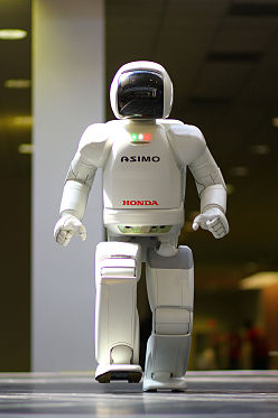
\includegraphics[width=0.2\textwidth]{figures/Introduccion/asimo.png}
		\caption{Robot Asimo}
		\label{fig.asimo}
		\end{center}
\end{figure}

El campo de la robótica es cada vez más popular y está en constante expansión. En la actualidad nos encontramos con múltiples ejemplos que integran la robótica en diferentes campos y tareas. Los robots comerciales e industriales son ampliamente utilizados y realizan tareas de forma más exacta o más barata que los humanos. Los robots, también, se emplean en trabajos demasiado sucios, peligrosos o tediosos para los humanos.\\

Hoy en día no solamente vemos robots industriales, como en cadenas de envasado de alimentos o cadenas de producción, sino que los robots cobran cada vez más importancia en los entornos domésticos. Las aspiradoras robóticas (Roomba, Dyson, Xiaomi…) han llegado a los hogares con éxito para facilitar una tarea doméstica necesaria. Los vehículos cada vez incorporan más tecnología robótica, como el aparcamiento automático en cualquier gama del mercado, asistentes de conducción autónoma (autopiloto de Tesla), o prototipos de coches autónomos que han lanzado grandes empresas como Google o Apple. Podemos ver robots en el campo de la medicina (como Da Vinci) que permiten operar siendo teleoperados desde cualquier parte del mundo; en el ámbito militar permitiendo desactivar bombas o realizar misiones rescate; en los almacenes de Amazon; o la creciente presencia de drones o robots aéreos.\\

Los robots tienen que interactuar con situaciones reales de forma robusta. Esto requiere que posean cierta inteligencia, la cual está presente en su software. Este software posee capas (\textit{drivers}, \textit{middleware} y aplicaciones), y presenta unas características diferentes según su aplicación. En los últimos años, se han incorporado a los robots ordenadores personales, micros de bajo coste y sistemas operativos generalistas.

\begin{figure}[H]
  \begin{center}
    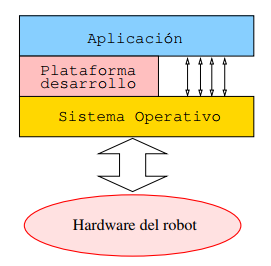
\includegraphics[width=0.4\textwidth]{figures/Introduccion/Esquema_Robot.png}
		\caption{Esquema del funcionamiento de un robot}
		\label{fig.Esquema_Robot}
		\end{center}
\end{figure}


\section{Software para robots}
Muchos robots poseen autonomía, la cual proviene del desarrollo de sistemas complejos, aplicaciones e infraestructuras que les dotan de inteligencia autónoma. El desarrollo de software robótico es similar al desarrollo de software en otros ámbitos, donde se parte de ciertos requisitos y se modela un diseño que será creado. Hace años el desarrollo de software robótico se realizaba adoptando soluciones ``ad hoc'', dotando a cada robot de un diseño específico, y con sensores y actuadores concretos. Esto suponía que no se podía aplicar el software desarrollado a otro robot, por lo que era necesario implementar de nuevo todo el software para un nuevo robot. En la actualidad, existen numerosas plataformas que permiten el desarrollo de aplicaciones robóticas de forma eficiente y genérica. Esto permite reutilizar gran parte de las aplicaciones creadas en otros robots, evitando el coste de realizar todo el proceso de nuevo.\\

Dotar al robot de cierta inteligencia conlleva desarrollar cierto software, el cual se suele programar apoyándose en herramientas, como los \textit{middleware} robóticos, los simuladores robóticos, o las  bibliotecas que facilitan algunos aspectos. A continuación, se exponen algunas de estas herramientas que se emplean en la actualidad.

\subsection{Middlewares robóticos}
En la actualidad existen numerosos \textit{middlewares} robóticos, que permiten gestionar la complejidad y heterogeneidad del hardware y las aplicaciones, promover la integración de nuevas tecnologías, simplificar el diseño de software, y ocultar la complejidad de los sensores. Algunos de los \textit{middlewares} robóticos más destacados son:

\begin{itemize}
\item \acrfull{ros} \footnote{\url{http://www.ros.org/}}~\cite{middleware1}: Es una plataforma de software libre para el desarrollo de software de robots, que provee servicios estándar de un sistema operativo como la abstracción del hardware, el control de dispositivos de bajo nivel, mecanismos de intercambio de mensajes entre procesos y un conjunto de herramientas utilizadas ampliamente en robótica. La librería está orientada para un sistema UNIX, aunque se está adaptando a otros sistemas operativos como Fedora, Mac OS X, Arch, Gentoo, OpenSUSE, Slackware, Debian o Microsoft Windows, considerados como ``experimentales''.
\item Orca \footnote{\url{http://orca-robotics.sourceforge.net/}}~\cite{middleware1}: Es una plataforma de software libre para el desarrollo de aplicaciones robóticas. Está orientada a componentes, los cuales se pueden ejecutar de manera independiente o conjunta para crear aplicaciones más complejas. Orca permite reutilizar código, de manera que se pueden emplear componentes robóticos ya creados.
\item Urbi~\cite{urbi}: Es una plataforma de software multiplataforma de código abierto en C++ utilizada para desarrollar aplicaciones para robótica y sistemas complejos. Urbi es compatible con \acrshort{ros} y se puede emplear en los sistemas operativos Linux, Windows y MAC OS X.
\end{itemize}

\subsection{Simuladores robóticos}
El diseño de un robot es costoso y caro, lo que implica que muchos componentes necesarios para la construcción de los robots solamente estén disponibles para centros de investigación y corporaciones. Cuando se emplea un robot puede que el código desarrollado falle al probarlo, pudiendo incluso romperse algún robot.\\

Hoy en día existen numerosos simuladores robóticos, lo que permite a cualquier persona crear, programar y probar infinidad de robots de forma segura y económica. Algunos de los simuladores más empleados son:

\begin{itemize}
\item Gazebo \footnote{\url{http://gazebosim.org/}}: Es un simulador 3D de código abierto distribuido bajo licencia Apache 2.0. Este simulador se ha utilizado en ámbitos de investigación en robótica e Inteligencia Artificial. Es destacado por sus motores de físicas, motor de renderizado avanzado, soporte para \textit{plugins}, un amplio repertorio de robots comerciales, y una extensa gama de sensores y actuadores. Es fácil de integrar con \acrshort{ros}.
\item Stage \footnote{\url{http://playerstage.sourceforge.net/doc/stage-svn/}}: Simula robots móviles en el plano bidimensional y proporciona diversos tipos de sensores y actuadores. Su finalidad es ayudar a la investigación de sistemas autónomos de múltiples agente, para lo cual proporciona gran cantidad de dispositivos simultáneamente.
\item Orocos \footnote{\url{http://www.orocos.org/taxonomy/term/18}}~\cite{orocos}~\cite{orocos1}: Es un proyecto de software libre para el control de robots y máquinas. Soporta 4 bibliotecas C++: Real-Time Toolkit, Kinematics and Dynamics Library,  Bayesian Filtering Library y  Orocos Component Library. Está orientado a componentes, permitiendo añadir funcionalidades de forma sencilla y sin recompilar todo el código.  Incluye paquetes complementarios tales como Filtros de Bayes, Librerías de control Dinámico y Cinemático o Visión. 
\item Webots \footnote{\url{https://www.cyberbotics.com/}}~\cite{webots}: Es un simulador avanzado de robótica, que permite definir modelos propios, definir la física, escribir controladores para los robots y hacer simulaciones a gran velocidad. Se puede emplear en los sistemas operativos Linux, Windows y MacOS. Los lenguajes de programación que se pueden emplear son  C++, C y Java.
\end{itemize}

\subsection{Bibliotecas}
En el desarrollo del software robótico es conveniente emplear bibliotecas que ya resuelven funcionalidades como el reconocimiento de gestos, procesamiento de imágenes, o la estimación de posición. En la actualidad existen diferentes bibliotecas que se emplean en robótica, por ejemplo:

\begin{itemize}
\item OpenCV \footnote{\url{http://opencv.org/}}: Está dirigida a la visión por computador en tiempo real. Entre las áreas de aplicación de esta biblioteca destacan: segmentación y reconocimiento de objetos, reconocimiento de gestos, seguimiento del movimiento, estructura del movimiento,  y robots móviles.
\item PCL \footnote{\url{http://pointclouds.org/}}~\cite{pcl}~\cite{pcl1}:Es una biblioteca de código abierto para el procesamiento de imágenes 2D/3D. Incluye numerosos algoritmos para manejar nubes  de puntos en N dimensiones, y procesamiento tridimensional de las mismas. Se emplea en el manejo de información en sensores RGBD como Kinect.
\item AForge.NET~\cite{AForge.NET}: Es un framework C\# de código abierto diseñado para desarrolladores e investigadores en los campos de Visión por Computadora e Inteligencia Artificial. Sus áreas de aplicación son: procesamiento de imágenes, redes neuronales, algoritmos genéticos, lógica difusa, aprendizaje de máquinas, robótica, etc.
\end{itemize}

\section{Docencia en robótica}
El propósito principal de este proyecto es la extensión de un entorno docente compuesto de varias prácticas para facilitar el aprendizaje de diferentes algoritmos de robótica. Estas prácticas utilizan técnicas robóticas próximas a las empleadas en la actualidad.\\

La robótica educativa es un medio de aprendizaje en el cual participan personas con motivación por el diseño y la construcción de creaciones propias. Esta disciplina se puede enseñar a estudiantes con muy diferentes niveles educativos. Ha crecido muy rápidamente en la última década y está en continuo desarrollo. Los robots están incorporándose en nuestra vida cotidiana, pasando de la industria a los hogares. El propósito de utilizar la robótica en la educación, a diferentes niveles de enseñanza, suele ir más allá de adquirir conocimiento en el campo de la robótica. Se pretende que el alumno sea capaz de aprender temas multidisciplinares (electrónica, informática, mecánica, física, etc), comprenda conceptos abstractos y complejos de ciencia y tecnología, y adquiriera competencias básicas que son necesarias en la sociedad de hoy día; como el aprendizaje colaborativo y la toma de decisión en equipo, entre otras.\\

La robótica genera entornos colaborativos donde los participantes pueden practicar las habilidades del siglo XXI, conocidas como las 4C:

\begin{itemize}
\item Creatividad: Implica generar nuevas ideas mejorando las que ya existen. Es necesario ponerse en diferentes puntos de vista en cada circunstancia, tener la mente abierta y ser receptivo ante nuevas ideas y conceptos. Ayuda a la resolución de problemas de manera más eficaz.
\item Pensamiento Crítico: Es imprescindible razonar con efectividad, claridad y precisión para desarrollar esta habilidad, reconociendo las conexiones que existen entre sistemas para resolver problemas y tomar decisiones. Se requiere practicar una correcta lógica de pensamientos para ver en cada situación los distintos puntos de vista.
\item Colaboración: Se basa en la capacidad para trabajar de forma eficaz y respetuosa en equipos diversos. Esta habilidad implica comprometerse con los demás en la consecución de un objetivo común. Es importante asumir la responsabilidad del trabajo colaborativo, así como las aportaciones de cada miembro del equipo.
\item Comunicación: Es la capacidad que permite intercambiar información de forma articulada, de dar y recibir retroalimentación de determinadas ideas con otras personas.
\end{itemize}

La robótica en la docencia intenta despertar el interés de los estudiantes transformando las asignaturas tradicionales en más atractivas e integradoras, ya que crea entornos de aprendizaje propicios que recrean los problemas del entorno que los rodea.\\

En el futuro, tener nociones básicas de esta disciplina será clave debido a que cada vez de forma más habitual se implantan robots en diferentes sectores laborales.

\subsection{Docencia en secundaria}

En los centros de enseñanza secundaria se imparte la robótica con frecuencia, ya que motiva a los alumnos. Esto les permite adquirir conocimientos tecnológicos, así como aprender conceptos básicos de ciencias, tecnología, ingeniería y matemáticas. Es decir, se implanta el enfoque de educación \textit{\acrfull{stem}}. El concepto \acrshort{stem} se ha desarrollado con el fin de enseñar Ciencias y Tecnología de forma conjunta. Este método tiene dos características fundamentales:

\begin{itemize}
\item Enseñanza-aprendizaje de tecnología, ciencias, ingeniería y matemáticas de forma conjunta e integrada.
\item Se da un enfoque a la tecnología de aprender conocimientos para resolver problemas tecnológicos reales. 
\end{itemize}

La enseñanza de robótica en secundaria se realiza mediante plataformas físicas como los robots LEGO (Mindstorms, RCX, NXT, Evo, WeDo), placas Arduino, los kits de SolidWorks, etc. Se suelen enseñar conceptos básicos de sensores y actuadores empleando lenguajes gráficos como RCXcode, Scratch y mbot Blockly. \\

En los últimos años, diferentes universidades han planteado cursos orientados a promover el diseño de robots en estudiantes de secundaria. Un ejemplo es el departamento de  Electrónica de la Universidad de Alcalá, que creó el proyecto ``TuBot'' con el fin de que los alumnos puedan construir su propio robot e incluso participar en una competición con el mismo.\\

Es importante destacar el curso JdeRobot-Kids \footnote{\url{http://jderobot.org/JdeRobot-kids}}, que emplea mbot como robot móvil, una placa programable Arduino, y Python como lenguaje para introducir a los jóvenes los conceptos básicos, de tecnología, robótica y programación. De esta forma los alumnos podrán aprender de una forma más divertida conceptos interesantes de informática, electrónica y mecánica. El curso es fundamentalmente práctico, ya que la mejor manera de aprender es creando.

\subsection{Docencia en la universidad}
En la docencia universitaria se imparten clases de robótica en los Grados y los Postgrados, en concreto en escuelas de ingeniería. La enseñanza de robótica o materias similares como la inteligencia artificial, la visión por computador o el aprendizaje automático, se pueden impartir en el ámbito industrial, pero también en el ámbito informático.\\

En España, podemos ver la robótica integrada en el ``Grado en Ingeniería Robótica'' de la Universidad de Alicante, donde nos encontramos con asignaturas como ``Iniciación a la ingeniería robótica'', ``Mecanismos y modelado de robots'', ``Programación de robots'', o ``Control de robots''. La enseñanza de robótica la podemos encontrar en los Grados de ''Electrónica industrial y automática'' que encontramos en numerosas universidades. Cabe destacar la universidad Carlos III de Madrid, donde se pueden estudiar materias como ``Robótica Industrial'' o ``Robótica''. En diversas universidades se puede estudiar el Grado ``Ingeniería Electrónica, Robótica y Mecatrónica''. Las universidades de Málaga y Sevilla cuentan con esta titulación, en la cual se imparten asignaturas como ``Fundamentos de Robótica'', ``Laboratorio de Robótica'', ``Robótica y Automatización'', o ``Ampliación de Robótica''.\\

En los estudios de Postgrado se imparten más asignaturas de robótica, puesto que es una enseñanza más especializada. Existen Másteres destacados como el ``Máster de Visión Artificial'', el ``Máster Universitario en Ingeniería Mecatrónica'', o el ``Máster Universitario en Automática y Robótica'' en diferentes universidades. Estos estudios de Postgrado los podemos encontrar en universidades como la Universidad Rey Juan Carlos, la Universidad Carlos III de Madrid, la Universidad del País Vasco, o la Universidad Politécnica de Cataluña.\\

En el ámbito internacional, algunas asociaciones prestigiosas como ACM (Association for Computing and Machinery) y la IEEE-CS (IEEE Computer Society) ven la robótica como un área de conocimiento imprescindible en estudios de ingeniería, informática y sistemas inteligentes. Se pueden destacar universidades especializadas en robótica como el MIT, Stanford, Georgia Institute of Technology, etc.\\

La asignatura de robótica habitualmente se imparte de forma práctica facilitando el aprendizaje de contenidos teóricos al alumno. Es común el uso de plataformas para la programación de robots. Algunas de las plataformas más destacadas son \acrshort{ros} \footnote{\url{http://www.ros.org/}}, o MATLAB con el paquete Simulink \footnote{\url{https://es.mathworks.com/products/simulink.html}}.\\

Cabe destacar The ConstructSim, que es útil para realizar simulaciones en la web. Esta plataforma web en la nube permite emplear una gran lista de simuladores por medio de un navegador web. De esta forma los usuarios no tienen que instalar nada, ni siquiera en sus navegadores.

\section{Entorno Docente JdeRobot-Academy}
La Universidad Rey Juan Carlos cuenta con el \textit{middleware} robótico JdeRobot, que tiene asociado un entorno académico conocido como JdeRobot-Academy. Este entorno educativo se ha empleado con éxito en diferentes asignaturas, como ``Visión en Robótica'' del Máster de Visión Artificial, o ``Robótica'' del Grado de Ingeniería Telemática. Asimismo, la Universidad ofrece cursos de introducción a la robótica y los drones, empleando dicha plataforma.\\

Los ejes principales de JdeRobot-Academy son: (a) lenguaje Python (por su sencillez y potencia), (b) simulador Gazebo (permite aprender robótica aunque no se disponga de robots reales, y permite tener un repertorio de robots variados ---drones, formula1, brazos, aspiradoras, etc.--- con los que enfocar aspectos muy variados de la robótica) y (c) foco en el algoritmo en vez de en el \textit{middleware} ocultando los detalles de la infraestructura.\\


El entorno cuenta con un conjunto de prácticas. En cada una se plantea un problema robótico que tiene que resolver el alumno. En ellas se pueden distinguir varias capas, que influyen en el desarrollo del diseño de las prácticas. La capa de nivel más bajo, que será la primera que se crea, es la creación de la infraestructura de la práctica, lo que supone la creación de los modelos necesarios, los \textit{plugins} que emplearán estos modelos, y el entorno simulado donde navegará el robot. \\

Por cada una de las prácticas se incluye un componente académico que le permitirá al alumno realizar la solución de las prácticas. Cada uno de estos componentes proporciona una interfaz gráfica (\acrshort{gui}) específica para esa práctica y código auxiliar de ayuda a la resolución de las prácticas. También suele incluir un evaluador automático, que permite llevar a cabo la corrección de las prácticas. En las prácticas se harán las conexiones necesarias del software del alumno con los sensores y actuadores que se empleen. El propósito de los componentes académicos es permitir la abstracción por parte de los alumnos de los elementos complejos que no son parte de la resolución de las prácticas. De esta forma, el alumno lo único que tendrá que hacer es programar la solución de cada algoritmo que se le propone.
\begin{figure}[H]
  \begin{center}
    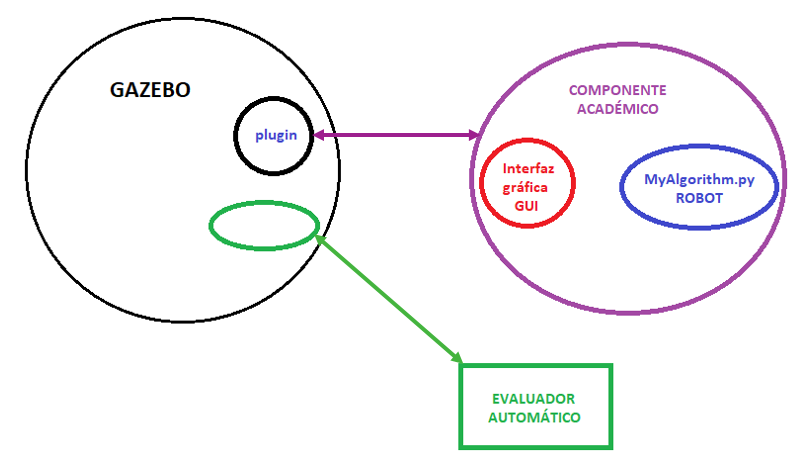
\includegraphics[width=1\textwidth]{figures/Introduccion/estructura.png}
		\caption{Estructura}
		\label{fig.estructura}
		\end{center}
\end{figure}

Se han creado los componentes académicos siguiendo una arquitectura software que permite facilitar el desarrollo de las prácticas a los alumnos, los cuales únicamente deberán realizar la solución, ya sea el pilotaje en función de los datos que proporcionan los sensores  o la realización de la planificación y el pilotaje. Los componentes cargan el código escrito por el alumno en el fichero \textit{MyAlgorithm.py} (donde se lleva a cabo la resolución), mostrando en la interfaz las pruebas o soluciones que realicen los alumnos. En la Figura~\ref{fig.estructura} podemos ver la estructura que tiene cada una de las prácticas.\\

Las prácticas se pueden realizar sobre robots simulados o reales, aunque lo más habitual es emplear robots simulados. Se apoyan en el simulador Gazebo, y se usa como lenguaje de programación Python. El principal sistema operativo para emplear esta plataforma es Linux. Sin embargo, se ha utilizado la interfaz web Gazebo para poder lanzarlo en Windows y MacOS mediante el empleo de Dockers.\\

A continuación, se presentan algunas de las prácticas ya desarrolladas en el entorno docente JdeRobot-Academy:

\begin{itemize}
\item Fórmula 1 \footnote{\url{https://www.youtube.com/watch?v=eNuSQN9egpA}}: sigue líneas. En esta práctica el alumno debe programar el comportamiento de un coche Fórmula 1 para que realice un control PID siguiendo la línea roja pintada en el circuito de carreras. Para ello el robot posee sensores de posición y una cámara. La interfaz de movimiento es simple puesto que admite órdenes de velocidad lineal o velocidad de giro.
\begin{figure}[H]
  \begin{center}
    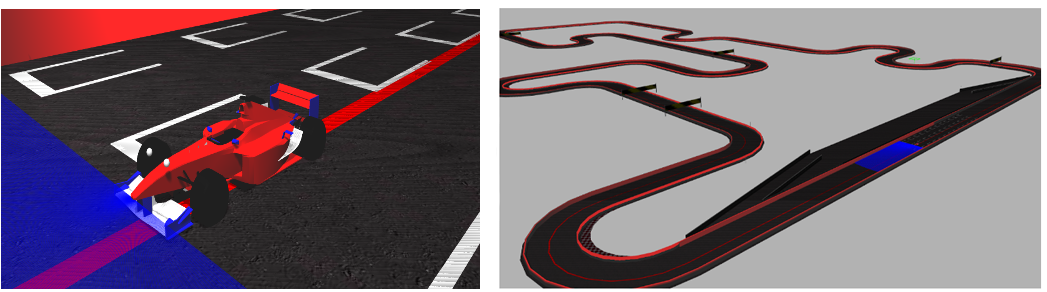
\includegraphics[width=0.8\textwidth]{figures/Introduccion/F1.png}
		\caption{Fórmula 1 y circuito de Gazebo}
		\label{fig.F1}
		\end{center}
\end{figure}
\item Visión \footnote{\url{http://jderobot.org/store/jmplaza/uploads/teaching/teachingrobotics-reconstruccion3D.mp4}}: reconstrucción 3D. En esta práctica el alumno debe lograr que un robot Pioneer reproduzca en 3D los elementos que están en frente del mismo. El robot cuenta con un par de cámaras estéreo. Para abordar el problema adecuadamente el alumno deberá programar un algoritmo de reconstrucción 3D clásico: detección de puntos de interés en el par de imágenes, emparejamiento de pixeles homólogos entre ambas, y triangulación espacial para calcular el punto tridimensional que origina cada pareja de pixeles homólogos. Esta práctica aborda técnicas de procesado de imagen y percepción visual.
\begin{figure}[H]
  \begin{center}
    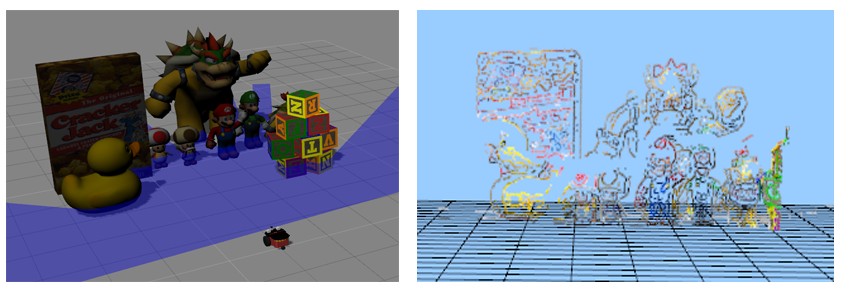
\includegraphics[width=0.8\textwidth]{figures/Introduccion/3D.png}
		\caption{Pioneer en el mundo de Gazebo y reconstrucción 3D}
		\label{fig.3D}
		\end{center}
\end{figure}
\item Control visual en drones \footnote{\url{https://www.youtube.com/watch?time_continue=96&v=BoDchf_6yMQ}}: sigue a la tortuga. En esta práctica el alumno debe conseguir que un drone siga a un robot Turtlebot que se desplaza por el suelo. Para lograr este objetivo el alumno deberá realizar los filtros de percepción visual necesarios para que el drone identifique al Turtlebot, así como programar el movimiento del drone para que siga al robot de forma adecuada. Esta práctica permite enseñar técnicas de percepción visual, de control reactivo, control basado en casos y de controladores PID.
\begin{figure}[H]
  \begin{center}
    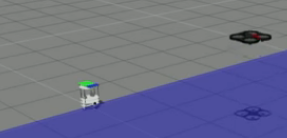
\includegraphics[width=0.5\textwidth]{figures/Introduccion/Tortuga.png}
		\caption{Drone en el mundo de Gazebo}
		\label{fig.Tortuga}
		\end{center}
\end{figure}
\end{itemize}

El objetivo general de este proyecto es ampliar las posibilidades de esta plataforma docente, creando nuevas prácticas y mejorando alguna ya existente. En los próximos capítulos abordaremos todos los elementos necesarios para conseguir este objetivo. En el Capítulo~\ref{cap.objetivos} cubriremos los objetivos que se han marcado en el proyecto, así como los requisitos para cumplirlos y la metodología empleada. En el Capítulo~\ref{cap.infraestructura} se expondrán la infraestructura utilizada durante el trabajo. En los Capítulos~\ref{cap.gpp},~\ref{cap.roomba} y~\ref{cap.autoparking}, se abordarán las prácticas que se han mejorado o creado. Por último, en el Capítulo~\ref{cap.conclusiones} se expondrán las conclusiones obtenidas al realizar el proyecto, así como las posibles líneas futuras a seguir.
\lhead[]{CAPÍTULO \thechapter. OBJETIVOS}
\chapter{Objetivos}\label{cap.objetivos}
Una vez explicado el contexto de este proyecto, se describirán en este capítulo los objetivos, los requisitos y la metodología que se han empleado.\\

\section{Objetivos}

El propósito principal de este proyecto es la creación o mejora de tres prácticas para el entorno docente JdeRobot-Academy. En concreto mejorar una práctica de navegación global, crear una práctica de una aspiradora robótica y, por último, crear una práctica acerca del aparcamiento de coches autónomos. Siguiendo el diseño de JdeRobot-Academy, para cada práctica hay que desarrollar 4 ingredientes:

\begin{itemize}
\item Enunciado e infraestructura en simulador
\item Componente académico que incluye \acrshort{gui} y código auxiliar
\item Solución de referencia
\item Evaluador automático
\end{itemize}

En cada una de estas prácticas se elaborará toda la infraestructura que se comunica con el Simulador Gazebo, donde el alumno podrá ver el resultado de la ejecución de su algoritmo. Se ofrecerá, en cada práctica, un fichero MyAlgorithm.py donde el alumno programará su solución.\\

Lo que difiere en estas tres prácticas es el escenario de cada una de ellas, los diferentes elementos que se mostrarán en el interfaz gráfico, los elementos que tendrá en cuenta el evaluador automático a la hora de calcular la nota de cada alumno, y por último el algoritmo concreto de la solución. Cada una de ellas es un subobjetivo de este proyecto.\\

Primero, en la práctica ``TeleTaxi'' el objetivo es que el alumno aprenda técnicas de navegación global, en concreto, la técnica \textit{Gradient Path Planning}. Está práctica no es totalmente original, sino que existía una versión previa de la infraestructura y del componente académico, pero presentaban ciertos problemas. Por ello, en este proyecto se va a mejorar tanto la infraestructura como el componente académico, así como se va a desarrollar una nueva solución de referencia y un evaluador automático que nos permita calificarla.\\

Segundo, en la práctica ``Aspiradora Autónoma'' el principal objetivo es que el alumno sea capaz de proporcionar una solución para la limpieza de una casa sin autolocalización. En concreto, este algoritmo de referencia se basará en el que ejecutan los modelos de la serie 500 de Roomba de iRobot. Se realizará una solución que limpia en función de tres modos de navegación: giro en espiral, seguimiento de paredes y cruce de habitación. La aspiradora cuenta con diferentes sensores y actuadores, entre los que se encuentran un sensor láser, un sensor bumper, y actuadores que permiten dar órdenes a la aspiradora de velocidad de tracción y velocidad de giro.  En este caso la práctica se ha realizado desde cero, pues no existía una versión previa. Con ella los alumnos se familiarizarán con un problema robótico real, cotidiano y cuya solución ya se está comercializando.\\


En último lugar, en la práctica ``Aparcamiento Automático'' el propósito es la realización de una solución que sea capaz de aparcar un coche de forma autónoma. El coche está dotado de tres sensores láser (que se encuentran en la parte frontal, en la parte trasera y en el lateral derecho) para medir distancias a los coches y encontrar aparcamiento. La solución propuesta es una solución ``ad hoc'' basada en las medidas sensoriales que se obtienen de los láseres. La solución permite al vehículo encontrar una plaza de aparcamiento libre y realizar la maniobra de aparcamiento. Esta práctica, también realizada de cero, nos permitirá acercarnos a sistemas robóticos que ya existen en el mercado (Volkswagen Tiguan, etc) y con ello aprender cómo funcionan.

\section{Requisitos}
El desarrollo del proyecto estará guiado por los subobjetivos mencionados anteriormente y deberá ajustarse a los requisitos de partida del proyecto, los cuales hacen que la solución esté condicionada. Estos requisitos son:

\begin{enumerate}[1.]
\item Todas las simulaciones se realizarán en el simulador Gazebo, en concreto en la versión 7. Los modelos de robots que se emplearán serán creados. En este caso se utilizarán dos taxis (los cuales tienen diferentes sensores) y el modelo Roomba.
\item Se hará uso del \textit{middleware} robótico JdeRobot en su versión 5.5.2, que se explicará con detalle en el siguiente capítulo~\ref{cap.infraestructura}. El uso de esta plataforma simplifica el desarrollo del comportamiento del robot. 
\item El sistema operativo que se empleará para este proyecto será Ubuntu 16.04.
\item El lenguaje de desarrollo empleado para crear los \textit{plugins} necesarios será C++. Sin embargo, en el resto de componentes se utilizará el lenguaje Python 2. Por compatibilidad con JdeRobot-5.5.2 y de éste con el \textit{middleware} ROS Kinetic no se ha usado Python-3.X, sino que se sigue Python-2.7.
\item Las soluciones han de ser vivaces. Los algoritmos propuestos no pueden detenerse mucho tiempo a pensar cuál será el próximo movimiento del robot, porque han de reaccionar rápido, en tiempo real y con movimientos suaves.
\end{enumerate}

\section{Metodología}
En el desarrollo del proyecto se ha seguido una metodología iterativa, donde cada iteración se compone de varias fases: determinar objetivos, planificación, diseño e implementación, análisis de riesgos, así como reuniones periódicas con el tutor.\\

Se ha optado por seguir el modelo de desarrollo en espiral, creado por Barry Boehm. Este modelo se adapta perfectamente a este tipo de proyectos, ya que permite separar el comportamiento final en varias subtareas más sencillas para después juntarlas. Este modelo permite una gran flexibilidad ante cambios en los requisitos, algo bastante común.\\

Este modelo de ciclo de vida permite ir obteniendo prototipos funcionales, a la vez que se realiza el desarrollo del producto de forma incremental. El modelo consta de iteraciones, que se pueden llamar ciclos. En cada ciclo existen cuatro fases bien diferenciadas:

\begin{itemize}
\item Determinar objetivos: Se definen los objetivos específicos que deben cumplirse para que el ciclo actual pueda considerarse finalizado en base a los objetivos finales. Conforme vayan sucediéndose más iteraciones, los objetivos serán más complejos.
\item Análisis del riesgo: Se efectúa un análisis detallado para cada uno de los riesgos que pueda tener el objetivo fijado en la fase anterior. Se definen los pasos a seguir para minimizar los riesgos y después del análisis se planean estrategias alternativas.
\item Desarrollar y probar: Se desarrolla el producto o las partes del producto que se han acordado en las fases anteriores. Además, se llevarán a cabo las pruebas oportunas que permitan asegurar la calidad de la implementación, y que pueda seguir sirviendo en iteraciones futuras.
\item Planificación: Se revisan los resultados obtenidos mediante las pruebas de la fase anterior, y es donde se planifica la iteración siguiente teniendo en cuenta los posibles errores que se han cometido.
\end{itemize}

\begin{figure}[H]
  \begin{center}
    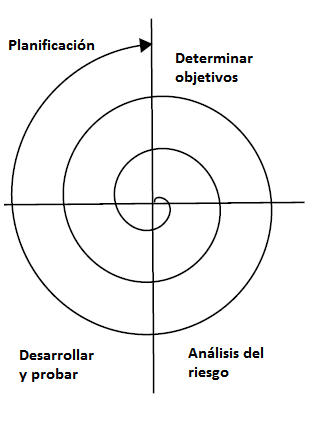
\includegraphics[width=0.4\textwidth]{figures/Objetivos/espiral.png}
		\caption{Modelo en espiral}
		\label{fig.espiral}
		\end{center}
\end{figure}

Para llevar a cabo esta metodología se han mantenido reuniones semanales con el tutor. En estas reuniones se analizaban los resultados de cada iteración, y en función de los resultados se fijaban nuevos objetivos y se planteaban posibles vías para resolverlos. El código que se ha ido desarrollando semanalmente se ha subido al repositorio propio público de Github \footnote{\url{https://github.com/RoboticsURJC-students/2016-tfg-vanessa-fernandez}}, que emplea el sistema de control de versiones. Además, las tareas realizadas se han ido mostrando semanalmente mediante explicaciones, vídeos o imágenes en la bitácora de la página de JdeRobot \footnote{\url{http://jderobot.org/Vmartinezf-tfg}}.\\

El resultado global de este TFG, las tres prácticas creadas, han sido integradas en el repositorio oficial de JdeRobot-Academy. Y están disponibles
como software libre.  

\section{Plan de trabajo}
Las etapas temporales en las que se ha dividido el proyecto, que además se corresponden con el modelo en espiral, son:

\begin{itemize}
\item Familiarización con el entorno JdeRobot y OpenCV. En esta etapa se ha descargado e instalado la plataforma JdeRobot, el entorno docente JdeRobot-Academy, y todo el software necesario para el desarrollo del proyecto. En esta fase se engloba el aprendizaje del uso de Github, para el control de versiones, y el aprendizaje básico de la librería OpenCV. Para cerrar esta fase se han realizado algunas soluciones de prácticas existentes del entorno JdeRobot-Academy.
\item Familiarización con el simulador Gazebo y sus \textit{plugins}. En esta etapa se ha estudiado código de la plataforma JdeRobot, así como el material disponible en Gazebo en la página oficial \footnote{\url{http://gazebosim.org/}}.  Además, se han realizado pruebas creando mundos simples en Gazebo mediante modelos ya disponibles. También se ha realizado un estudio de los \textit{plugins} creados en JdeRobot (compilación e instalación), aprendizaje básico de C++, y desarrollo de algún \textit{plugin} necesario para el desarrollo de las prácticas.
\item Desarrollo de la práctica ``TeleTaxi'': Desarrollo del enunciado, la infraestructura en gazebo, el componente académico, la solución de referencia y
el evaluador automático.
\item Desarrollo de la práctica ``Aspiradora Autónoma'': Desarrollo del enunciado, la infraestructura en gazebo, el componente académico, la solución de referencia y el evaluador automático.
\item Desarrollo de la práctica ``Aparcamiento automático'': Desarrollo del enunciado, la infraestructura en gazebo, el componente académico, la solución de referencia y el evaluador automático.
\end{itemize}
\lhead[]{CAPÍTULO \thechapter. INFRAESTRUCTURA}
\chapter{Infraestructura}\label{cap.infraestructura}
En este capítulo se explican los principales ingredientes software en los que nos hemos apoyado  para desarrollar el trabajo. Tales como el entorno JdeRobot, el simulador Gazebo (con el cual podemos simular las acciones que realizaría un robot en un mundo determinado), la librería de OpenCV (empleada en todo lo relacionado con el tratamiento de imagen), PyQt (para el desarrollo de la interfaz gráfica) y Python como lenguaje de programación.

\section{Simulador Gazebo}
Gazebo es un simulador usado en robótica que permite realizar diversos escenarios tridimensionales donde probar nuestro software. A la hora de realizar el software es necesario hacer pruebas, las cuales saldrían muy caras si se probarán en robots reales (podría no funcionar correctamente y que nuestro robot se rompiera). Por esta razón es muy útil el empleo de simuladores, pues podemos realizar las pruebas que queramos sin peligro de que nuestro robot salga herido. Con los simuladores se pueden diseñar robots y escenarios realistas donde ejecutar nuestros algoritmos.

\begin{figure}[H]
  \begin{center}
    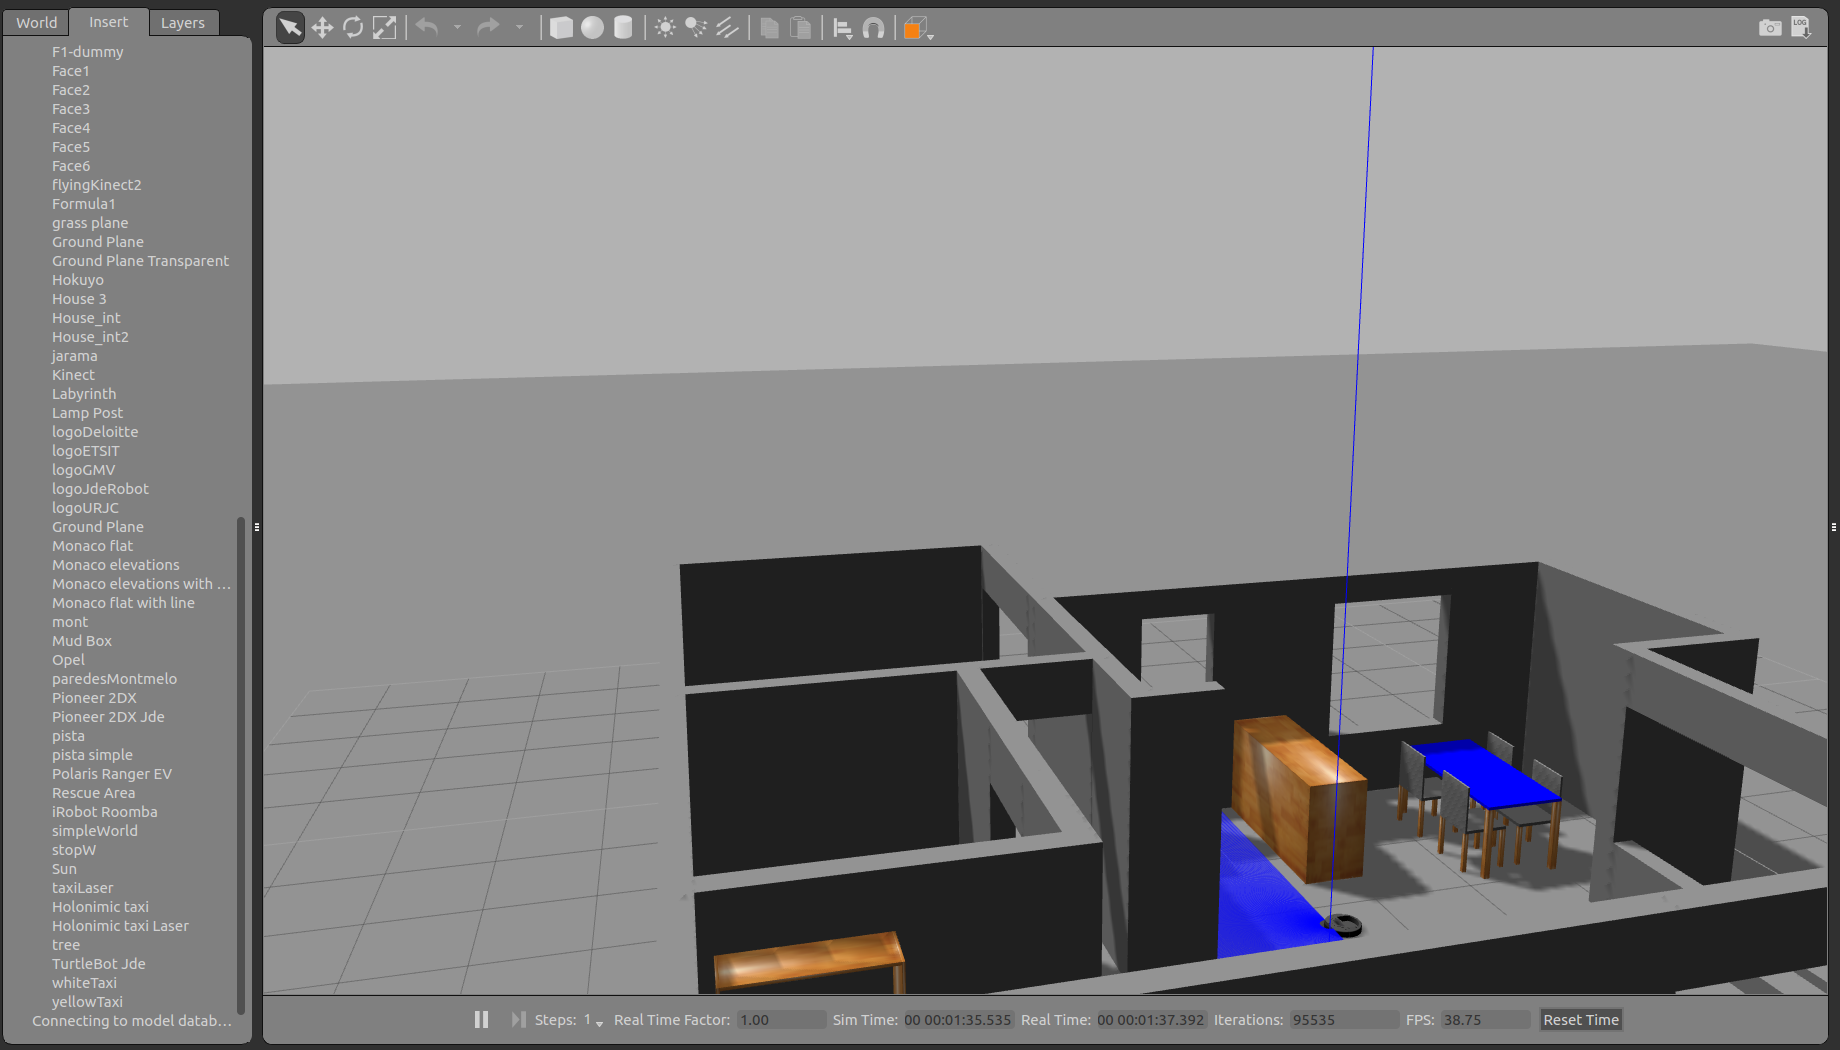
\includegraphics[width=0.7\textwidth]{figures/Infraestructura/gazebo.png}
		\caption{Simulador Gazebo}
		\label{fig.gazebo}
		\end{center}
\end{figure}

Gazebo es un programa de código abierto distribuido bajo licencia de Apache 2.0. Como se argumentó en el capítulo 1 es uno de los ejes de JdeRobot-Academy.  Se emplea en el desarrollo de aplicaciones robóticas y en inteligencia artificial. Es capaz de simular robots, objetos y sensores en entornos complejos de interior y exterior. Tiene gráficos de gran calidad y un robusto motor de física (masa del robot, rozamiento, inercia, amortiguamiento, etc.). Fue elegido para realizar el DARPA Robotics Challenge (2012--2015) y está mantenido por la Fundación Robótica de Código Abierto (OSRF).\\

En este trabajo se emplea la versión 7 de Gazebo \footnote{\url{http://gazebosim.org/blog/gazebo7}}, la cual se usará para crear los diferentes entornos y para probar nuestros algoritmos.  Gracias a Gazebo se pueden incluir texturas, luces y sombras en los escenarios, así como simular física como por ejemplo choques, empujes, gravedad, etc. Además, incluye diversos sensores, como pueden ser cámaras y lásers, los cuales podrán ser incorporados en los robots que empleemos. Todo ello hace que sea una herramienta muy potente y de gran ayuda en el mundo de la robótica.\\

Los mundos simulados con Gazebo son mundos 3D, que se cargan a partir de ficheros con extensión ``.world''. Estos ficheros son fichero \acrfull{xml} definidos en el lenguaje \acrfull{sdf}. Este lenguaje contiene una descripción completa de todos los elementos que tiene el mundo y los robots, incluyendo:

\begin{itemize}
\item Escena: Luz ambiente, propiedades del cielo, sombras, etc.
\item Mundo: Representa el mundo como un conjunto de modelos, plugins y propiedades físicas.
\item Modelo: Links, joint, objetos de colisión, sensores, etc.
\item Físicas: Gravedad, motor físico, paso del tiempo, colisiones, inercias, etc.
\item Plugins: Sobre un mundo, modelo o sensor.
\item Luz: Los puntos y origen de la luz.
\end{itemize}

Las etiquetas empleadas en el fichero para representar estos elementos son: Scene, World, Model, Physics, Plugin, y Ligth.\\

Los modelos de robots que se emplean en la simulación son creados mediante algún programa de modelado 3D (Blender, Sketchup…). Estos robots simulados necesitan ser dotados de inteligencia para lo cual se emplean los plugins. Estos plugins pueden dotar al robot de inteligencia u ofrecer la información de sus sensores a aplicaciones externas y recibir de éstas comandos para los actuadores de los robots.


\section{Entorno JdeRobot}
JdeRobot\footnote{\url{http://jderobot.org/Main_Page}} es una plataforma de software libre para el desarrollo de aplicaciones con robots y visión artificial. Esta plataforma fue creada por el Grupo de Robótica de la Universidad Rey Juan Carlos en 2003 y está licenciada como GPLv3.\\

Está desarrollado en C y C++, aunque contiene componentes desarrollados en lenguajes como Python y Java. El entorno que ofrece está basado en componentes, los cuales se ejecutan como procesos. Dichos componentes interoperan entre sí a través del middleware de comunicaciones \acrshort{ice}. \acrshort{ice} permite la interoperación entre los componentes incluso estando desarrollados en diferentes lenguajes.\\

Es capaz de llevar a cabo diferentes tareas en tiempo real de forma sencilla. Cada componente driver está asociado a un dispositivo hardware del robot, e incluye funciones para poder emplearlo. Esto simplifica el acceso a los diferentes componentes hardware, ya que con una simple función se puede acceder a ellos.\\

Las aplicaciones constan de uno o varios componentes. Los que interactúan directamente con los sensores y actuadores del robot se llaman drivers, que son los encargados de controlar que los robots reciben órdenes a través de interfaces \acrshort{ice} o \acrshort{ros} messages. Otros llevan en su código las funciones perceptivas, procesamiento de señales o la lógica de control e inteligencia del robot. En la siguiente imagen se puede ver un ejemplo de esta comunicación con un AR Drone empleando interfaces \acrshort{ice}. La misma lógica de comportamiento se puede conectar al driver del drone real o al driver del drone simulado. Basta con cambiar la configuración.

\begin{figure}[H]
  \begin{center}
    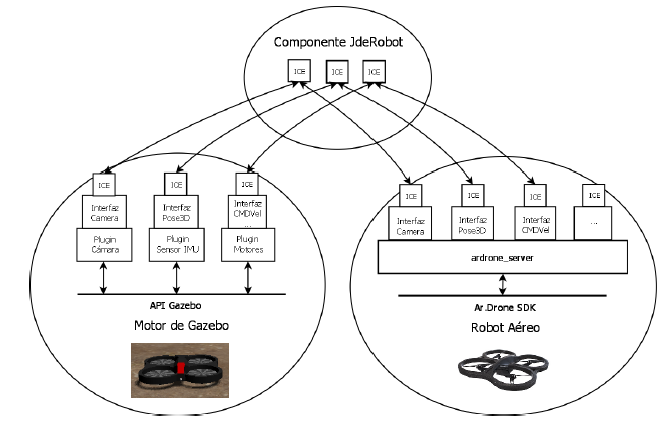
\includegraphics[width=0.7\textwidth]{figures/Infraestructura/jderobot.png}
		\caption{Ejemplo de componentes JdeRobot }
		\label{fig.jderobot}
		\end{center}
\end{figure}
En el ejemplo de la imagen se puede ver como los componentes de JdeRobot se comunican mediante \acrshort{ice} con los elementos del círculo izquierdo y con los del círculo derecho. En el círculo izquierdo se encuentran los dispositivos del robot simulado en Gazebo, que en este caso son una cámara, un sensor de posición y los motores. En el círculo derecho están los componentes de un robot real. Con esto podemos ver que con JdeRobot se puede teleoperar tanto con un robot simulado como uno real.\\

Esta plataforma soporta gran variedad de dispositivos como pueden ser el cuadricóptero AR Drone de Parrot, el robot Pioneer de MobileRobotics Inc., el robot Kobuki de Yujin Robot, el humanoide NAO de Aldebaran Robotics, cámaras firewire, USB e IP, los escáneres laser LMS de SICK y URG de Hokuyo, los simuladores Stage y Gazebo, sensores de profundidad como kinect y otros dispositivos X10 de dómotica. A parte de todo esto, tiene soporte para software externo como OpenCV, OpenGL, XForms, GTK, Player y GSL.   \\

En el desarrollo de las prácticas se empleará la versión 5.5.2 de JdeRobot, ya que es la última versión estable.


\section{Python}
Python\footnote{\url{https://www.python.org/}} se trata de un lenguaje de programación fácil de aprender y de alto nivel. Su creador fue Guido van Rossum, un investigador holandés que trabajaba en el centro de investigación CWI (Centrum Wiskunde \& Informatica). La primera versión surgió en 1991 pero no fue publicado hasta tres años después. Guido dio el nombre de Python en honor a la serie de televisión  \textit{Monty Python’s Flying Circus}.\\


Python incluye orientación a objetos, manejo de excepciones, listas, diccionarios, etc. A pesar de todo lo que soporta, se creó con el objetivo de que fuera un lenguaje sencillo de entender, sin perder todas las funcionalidades que pueden ofrecer lenguajes complejos tales como C.\\

Actualmente Python se trata de un lenguaje de código abierto administrado por Python Software Foundation. Este lenguaje incluye módulos que permiten la entrada y salida de ficheros, sockets, llamadas al sistema e incluso interfaces graficas como GTK y Qt. Además, permite dividir el programa en módulos reutilizables y no es necesario compilarlo, pues es un lenguaje de programación interpretado. Como se argumentó en el capítulo 1 es uno de los ejes de JdeRobot-Academy.\\

La última versión ofrecida por Python Software Foundation es la 3.6.2 , pero en nuestro caso se empleará la 2.7.12 por compatibilidad con JdeRobot 5.5.2, que a su vez sigue en esa versión de Python para ser compatible con \acrshort{ros} Kinetic. El código en el que están escritos los componentes académicos y las soluciones es Python.

\section{OpenCV}
OpenCV\footnote{\url{http://opencv.org/}} es una librería de código abierto desarrollada por Intel y publicada bajo licencia de BSD. Esta librería implementa gran variedad de herramientas para la interpretación de la imagen. Sus siglas provienen de los términos anglosajones ``Open Source Computer Vision Library'', es una librería destinada a aplicaciones de visión por computador en tiempo real.  \\

Esta librería puede ser usada en MAC, Windows, Android y Linux, y existen versiones para C\#, Python y Java, a pesar de que originalmente era una librería en C/C++. Además, hay interfaces en desarrollo para Ruby, Matlab y otros lenguajes.\\

OpenCV es una librería que principalmente implementa algoritmos para las técnicas de calibración, detección de rasgos, para el rastreo, análisis de la forma, análisis del movimiento, reconstrucción 3D, segmentación de objetos y reconocimiento. Los algoritmos se basan en estructuras de datos flexibles acopladas con estructuras IPL (Intel Image Processing Library), aprovechándose de la arquitectura de Intel en la optimización de más de la mitad de las funciones.  \\

Fue diseñado para tener una alta eficiencia computacional. Está escrito en C y puede aprovechar las ventajas de los procesadores multinúcleo. La biblioteca de OpenCV contiene más de 500 funciones que abarcan muchas áreas de la visión artificial. También tiene una librería de aprendizaje automático (MLL, Machine Learning Library) destinada al reconocimiento y agrupación de patrones estadísticos. 

\begin{figure}[H]
  \begin{center}
    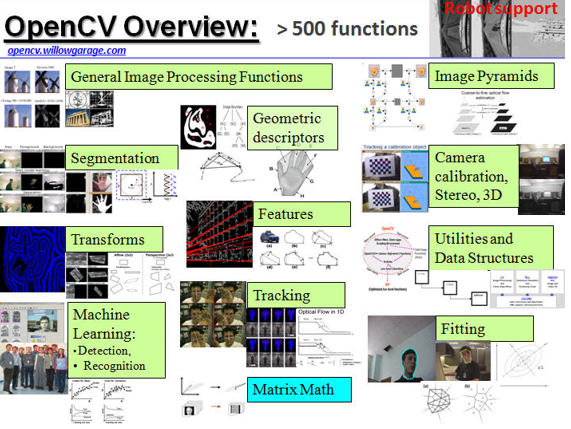
\includegraphics[width=0.6\textwidth]{figures/Infraestructura/opencv.png}
		\caption{Funciones de OpenCV }
		\label{fig.opencv}
		\end{center}
\end{figure}

OpenCV está compuesto por numerosas librerías con las cuales podemos manejar estructuras de datos, detectar bordes y esquinas, escalar o rotar imágenes, modificar el espacio de color de una imagen, realizar matching (comparación de formas para poder saber el parecido entre dos imágenes), detectar líneas y círculos, tratar objetos en 3D, crear ventanas y asociar eventos a dichas ventanas, etc. Incorpora funciones básicas para modelar el fondo, sustraer dicho fondo, generar imágenes de movimiento MHI (Motion History Images), etc. Además, incluye funciones para determinar dónde hubo movimiento y en qué dirección. \\


Desde su aparición OpenCV ha sido usado en numerosas aplicaciones. Entre las cuales se encuentran la unión de imágenes de satélites y de mapas web, la reducción de ruido en imágenes médicas, los sistemas de detección de movimiento, la calibración de cámaras, el manejo de vehículos no tripulados, el reconocimiento de gestos, etc. \\

Hay una gran cantidad de empresas y centros de investigación que emplean estas técnicas como IBM, Microsoft, Intel, SONY, Siemens, Google, Stanford, MIT, CMU, Cambridge e INRIA.\\

En este trabajo se ha empleado la versión 3.2 de OpenCV en Python. Esta librería se empleará para realizar todo lo relacionado con el tratamiento de imágenes. Con ello se extraerán datos que puedan emplearse a la hora de tomar decisiones para que los robots funcionen correctamente.

\section{PyQt}
PyQt~\cite{python1} ~\cite{pqt} es un conjunto de enlaces Python para el conjunto de herramientas Qt, las cuales se emplean para el desarrollo de la interfaz gráfica. Fue desarrollado por Riverbank Computing Ltd y es soportado por Windows, Linux, Mac OS/X, iOS y Android.\\

Qt es un entorno multiplataforma orientado a objetos desarrollado en C++  que permite desarrollar interfaces gráficas e incluye sockets, hilos, Unicode, bases de datos SQL, etc. PyQt combina todas las ventajas de Qt y Python, pues permite emplear todas las funcionalidades ofrecidas por Qt con un lenguaje de programación tan sencillo como Python.\\

En este proyecto se ha empleado la versión 5 de PyQt. PyQt5 es un conjunto de enlaces Python para Qt5, disponible en Python 2.x y 3.x. Tiene más de 620 clases y 6000 funciones y métodos. PyQt5 dispone de una licencia dual, es decir, los desarrolladores pueden elegir entre una licencia GPL (General Public Licence) o una licencia comercial. \\

La interfaz gráfica de los componentes académicos creados en las prácticas está escrita usando PyQt. Las clases de PyQt5 se dividen en ciertos módulos, tales como QtCore, QtGui, QtWidgets, QtXml, QtSql, etc. En las prácticas desarrolladas se ha hecho uso de los siguientes módulos:

\begin{itemize}
\item QtCore: contiene las funcionalidades principales que no tienen que ver con la \acrshort{gui}. Este módulo se emplea para trabajar con archivos, diferentes tipos de datos, hilos, procesos, url, etc.
\item QtGui: contiene clases para el desarrollo de ventanas, gráficos 2D, imágenes y texto.
\item QtWidgets: dispone de clases que proporcionan un conjunto de elementos de interfaz de usuario para crear interfaces de usuario clásicas de escritorio. 
\end{itemize}
\lhead[]{CAPÍTULO \thechapter. GPP}
\chapter{Práctica: Navegación global de un TeleTaxi con GPP}\label{cap.gpp}
 Una vez explicado el contexto, los objetivos y las herramientas empleadas en este proyecto, en este capítulo se detallarán las mejoras de infraestructura y componente académico en la práctica de JdeRobot-Academy denominada ``\textit{TeleTaxi}'', así como el evaluador automático creado y la nueva solución de referencia realizada. Esta práctica ya formaba parte del entorno JdeRobot-Academy, pero se han realizado diferentes mejoras que se describirán a lo largo del capítulo.

\section{Enunciado} \label{sec.enunciado}
El propósito de esta práctica es que un taxi autónomo sea capaz de navegar desde un punto de la ciudad a cualquier otro punto donde tiene que recoger o soltar a un cliente. El usuario humano podrá especificar un punto de destino al robot (taxi) picando con el ratón en algún lugar de la ciudad, cuyo mapa también se muestra en el interfaz gráfico del componente académico. El taxi dispondrá de un mapa de la ciudad y un sensor \textit{\acrfull{gps}} que le proporciona una estimación de su posición en la ciudad. Este vehículo posee un actuador de movimiento basado en velocidad lineal y velocidad de giro.\\ 

El alumno deberá programar el algoritmo de navegación global \acrfull{gpp} para obtener una planificación de la ruta que ha de seguir desde la posición actual del robot hasta la posición destino definida por el usuario en la interfaz gráfica (\acrshort{gui}). Una vez calculada la ruta más corta entre los puntos mencionados, en el \acrshort{gui} se podrá visualizar la ruta en el mapa 2D, así como una imagen con el campo de gradiente calculado por el código del alumno (nos dará información acerca de la ruta en función de la distancia). Una vez calculada la ruta, el alumno deberá proporcionar un algoritmo de pilotaje para que el robot la siga. Este algoritmo deberá tener en cuenta el campo calculado mediante el \acrshort{gpp} y la posición del taxi. 

\section{Infraestructura}
En este punto se comentará el entorno creado para llevar a cabo la práctica. Comenzamos con una descripción del robot que se ha empleado para el desarrollo de la práctica, así como una descripción de los actuadores y sensores que posee este robot, y una explicación de la ciudad por la que se moverá nuestro robot.

\subsection{Coche Taxi\_Holo}
El robot que se ha empleado en esta práctica es un nuevo modelo de robot creado en un programa de modelado 3D (como pueden ser Blender, SketchUp, etc). La versión anterior de ``TeleTaxi'' usaba el modelo \textit{yellowTaxi}, el cual es un robot creado para poder moverse de forma autónoma o teledirigida por un escenario. El nuevo modelo \textit{Taxi\_Holo} posee sensores \acrshort{gps} que le permiten saber cuál es su posición en todo momento; así como motores que le permite moverse por el escenario de manera adecuada. No posee otros sensores como pueden ser cámaras o láseres.\\

El modelo \textit{yellowTaxi} de la versión antigua de la práctica ``TeleTaxi'' es realista, tiene en cuenta las características propias de un automóvil, pero con el aspecto de un taxi. Este robot posee unas dimensiones grandes, ya que mide aproximadamente 5.75 metros de largo, 3 metros de ancho y posee una altura de 3 metros (Figura~\ref{fig.teleTaxi}).  Una característica importante de este modelo es que es  holonómico \footnote{Holonómico quiere decir que puede girar en el sitio sin chocar con nada.}. Este coche  se puede ver en la figura ~\ref{fig.teleTaxi}.

\begin{figure}[H]
  \begin{center}
    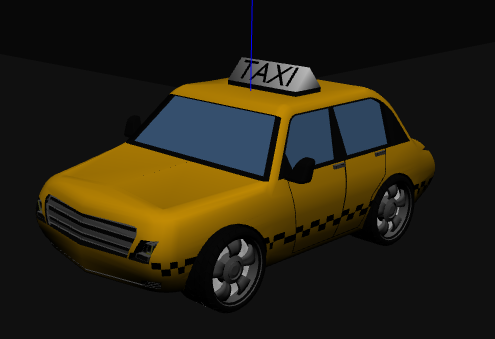
\includegraphics[width=0.3\textwidth]{figures/GPP/gpp_teleTaxi.png}
		\caption{Modelo yellowTaxi}
		\label{fig.teleTaxi}
		\end{center}
\end{figure}

Este modelo tenía fallos en su estructura que hacían que apenas se pudiera desplazar en el mundo o no fuera capaz de rotar, aunque le enviáramos órdenes de velocidad de tracción y velocidad de rotación muy elevadas. Este inconveniente suponía que el taxi tardara mucho tiempo en llegar a un objetivo cercano o que fuera incapaz de girar suficiente en las curvas, lo que hacía que se chocara contra las paredes de los obstáculos. Por este motivo, se creó un nuevo modelo de taxi denominado \textit{taxi\_holo}.\\

El nuevo modelo de taxi (Figura~\ref{fig.coche_holo}), el cual ha sido creado por desarrolladores del proyecto JdeRobot, cuenta con sensores de \acrshort{gps} y motores que permiten el movimiento al igual que el modelo antiguo. Es capaz de moverse de forma fluida por el escenario. Posee unas dimensiones de menor tamaño, 4 metros de largo, 2 metros de ancho y una altura de 1.5 metros. Este taxi pesa 750 kg y es también holonómico como el anterior, pero resuelve de forma eficiente los problemas de movimiento que tenía el antiguo modelo. 

\begin{figure}[H]
  \begin{center}
    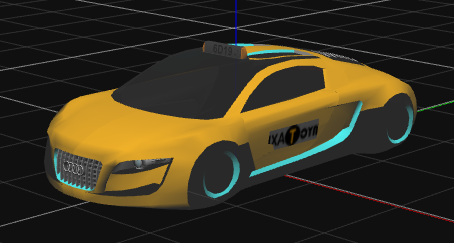
\includegraphics[width=0.3\textwidth]{figures/GPP/Coche_holo.png}
		\caption{Modelo taxi\_holo}
		\label{fig.coche_holo}
		\end{center}
\end{figure}

Los sensores de posición (tipo \acrshort{gps}, odometría u otros) que incorpora el taxi son ampliamente utilizados, ya que son una gran fuente de información para los algoritmos en los que se apoya el pilotaje de nuestro robot. La odometría se emplea para estimar la posición (x, y, orientación) de un robot móvil en todo momento. La posición estimada es relativa a la localización inicial del robot. Por tanto, emplearemos estos sensores de posición para estimar la posición del taxi en el mundo, y a partir de este dato estimar su velocidad.  Los sensores de odometría estiman la posición de las ruedas izquierda y derecha en un intervalo de tiempo determinado. Al conocer las coordenadas de posición anteriores resulta más sencillo obtener la nueva posición de nuestro robot. La plataforma JdeRobot aísla de la complejidad que conllevan los sensores de odometría, facilitándonos una variable que contiene la posición (x, y, orientación) en el mundo.\\


En esta práctica se han empleado dos \textit{plugins} asociados al taxi simulado: 

\begin{itemize}
\item \textit{holoCarPose3d}: Es el \textit{plugin} que emplearán los componentes para poder obtener su posición en tiempo real. También se utiliza para cambiar mágicamente la posición del taxi en el mundo simulado.
\item \textit{holoCarMotors}: Es el \textit{plugin} que permite dotar al taxi de velocidad, tanto velocidad de tracción como velocidad de rotación. 
\end{itemize}

\subsection{Modelo de ciudad cityLarge}
El objetivo de esta práctica es que nuestro taxi sea capaz de navegar por una ciudad hasta un punto destino, por lo que tendremos que crear el entorno (ciudad) donde se moverá. Con este propósito se ha creado un modelo de ciudad llamado \textit{“cityLarge”}. Este modelo fue creado con una herramienta de modelado 3D (Blender). El modelo cityLarge se corresponde con una ciudad de grandes dimensiones. En esta ciudad no veremos casas, semáforos, parques u otros elementos habituales en las ciudades reales, sino que se ha simplificado su creación para que sea rápido en la ejecución del simulador. Mundos con mucho detalle son más costosos computacionalmente de simular. Lo que podremos ver en esta ciudad son bloques que se corresponden con manzanas de edificios o carreteras. También podemos ver elementos propios de las carreteras como son rectas, curvas más simples o curvas pronunciadas, así como una zona amplia que se corresponde con una especie de plaza.  \\

Este modelo se ha modificado respecto a la versión antigua, debido a que en dicha versión debajo de la ciudad había un palo de sujección. Este elemento hacía que el coche adquiriera un poco de movimiento adicional al ejecutar la práctica. Por lo tanto, se ha eliminado este palo de sujeción. \\

En la Figura~\ref{fig.mundo_palo} podemos ver la parte de debajo del modelo \textit{cityLarge} para observar que había un palo de sujeción de la ciudad. En la Figura~\ref{fig.mundo_sinpalo} se observa el nuevo modelo \textit{cityLarge} sin dicho elemento de sujeción. Por último, en la Figura~\ref{fig.citiLarge} tenemos un plano desde arriba de toda la ciudad.

\begin{figure}[H]
  \begin{center}
    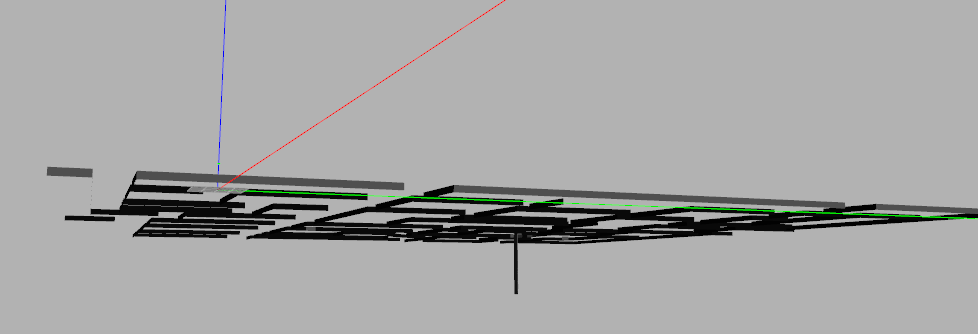
\includegraphics[width=0.6\textwidth]{figures/GPP/Mundo_palo.png}
		\caption{Modelo antiguo cityLarge}
		\label{fig.mundo_palo}
		\end{center}
\end{figure}

\begin{figure}[H]
  \begin{center}
    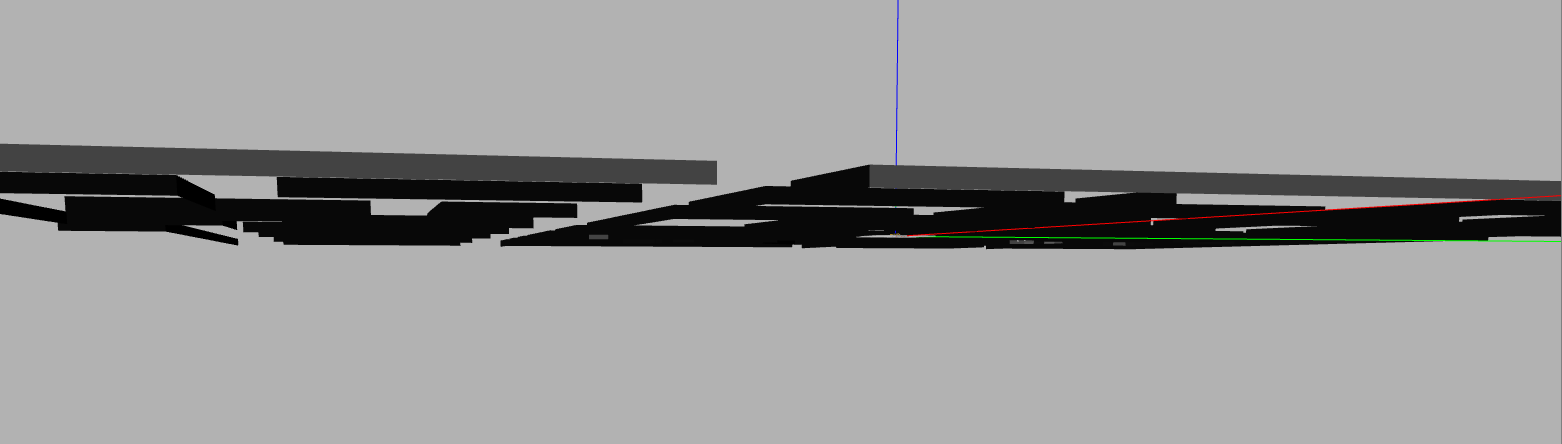
\includegraphics[width=0.6\textwidth]{figures/GPP/Mundo_sinPalo.png}
		\caption{Modelo nuevo cityLarge}
		\label{fig.mundo_sinpalo}
		\end{center}
\end{figure}

\begin{figure}[H]
  \begin{center}
    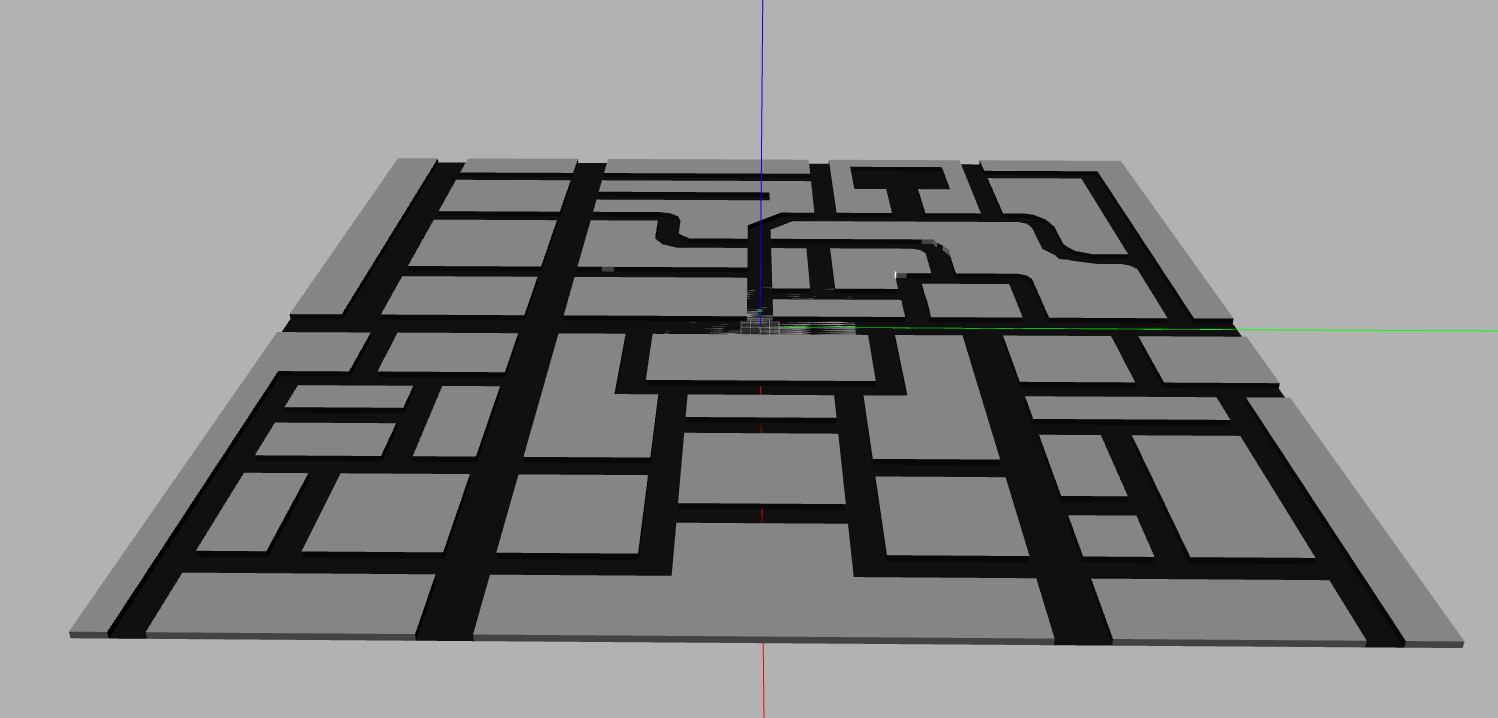
\includegraphics[width=0.5\textwidth]{figures/GPP/citiLarge_modelo.png}
		\caption{Modelo cityLarge desde arriba}
		\label{fig.citiLarge}
		\end{center}
\end{figure}

\subsection{Mundo de Gazebo}
Los mundos que se simulan con Gazebo son mundos 3D. Estos mundos se cargan en ficheros con extensión .world, que no son más que ficheros \acrshort{xml} definidos en el lenguaje \acrshort{sdf}. Este lenguaje contiene una descripción completa de todos los elementos que tiene el mundo y los robots.\\


Se ha creado un mundo en Gazebo (\textit{cityLarge.world}) compuesto por el modelo de la ciudad (\textit{cityLarge}) y el modelo del taxi (\textit{taxi\_holo}). El antiguo mundo en vez de utilizar el modelo \textit{taxi\_holo} empleaba el modelo \textit{yellow\_taxi}. El archivo \textit{cityLarge.world} tiene el siguiente aspecto:

\vspace{20pt}
	\begin{lstlisting}[frame=single]
<?xml version="1.0" ?>
  <sdf version="1.4">
    <world name="cityLarge">
      <!-- My city -->
      <include>
        <uri>model://cityLarge</uri>
      </include>
      <!-- My robots -->
      <include>
        <uri>model://taxi_holo</uri>
        <pose>0 0 0 0 0 0</pose>
      </include>
      <!-- A global light source -->
          <include>
            <uri>model://sun</uri>
      </include>
    </world>
  </sdf>

	\end{lstlisting}

\section{Componente Académico}
El componente académico para ayudar al alumno y alojar su código en esta práctica resuelve varias funcionalidades: (a) ofrece una interfaz gráfica al estudiante que le ayuda a depurar su código; (b) ofrece acceso a sensores y actuadores en forma de métodos simples (oculta el \textit{middleware} de comunicaciones); (c) incluye código auxiliar que no es el foco del algoritmo pero que ayuda a programar la solución. Lo deja todo atado para que el estudiante sólo tenga que incluir su código retocando el fichero \textit{MyAlgorithm.py}.\\

Este componente ofrece al programador del algoritmo un \acrfull{api} de sensores y actuadores. A continuación se puede ver el \acrshort{api} concreto de esta práctica:

\begin{itemize}
\item \textit{sensor.getRobotX()}: Permite obtener la posición del robot en el eje X.
\item \textit{sensor.getRobotY()}: Permite obtener la posición del robot en el eje Y.
\item \textit{sensor.getRobotTheta()}: Permite obtener la orientación del robot con respecto al mapa.
\item \textit{vel.setV()}: Para establecer la velocidad lineal.
\item \textit{vel.setW()}: Para establecer la velocidad de giro.
\end{itemize}

Es necesario escribir un archivo de configuración para que este componente pueda comunicarse con gazeboserver. En este fichero se indican los puertos de los \textit{plugins} que usa el taxi. Este fichero (\textit{teleTaxi.cfg}) en la práctica tiene el siguiente aspecto.

\vspace{20pt}
	\begin{lstlisting}[frame=single]
TeleTaxi.Motors.Proxy = Motors:default -h localhost -p 9999
TeleTaxi.Pose3D.Proxy = Pose3D:default -h localhost -p 9989
TeleTaxi.robot=Pioneer

TeleTaxi.Motors.maxV = 50
TeleTaxi.Motors.maxW = 20

	\end{lstlisting}

Podemos ver que los motores emplean el Puerto 9999, mientras que la pose3d emplea el Puerto 9989. Además, se puede ver en este archivo que se indica al robot la velocidad máxima de tracción y de rotación.\\


Se ha dividido el trabajo de este componente académico en diferentes partes, por lo que emplearemos hilos de ejecución para llevar a cabo diferentes tareas simultáneamente. En esta práctica existen dos procesos diferenciados:

\begin{itemize}
\item Hilo de control: Este hilo es el encargado de actualizar los datos de los sensores y los actuadores a través de las interfaces \acrshort{ice}. El tiempo de refresco de este hilo es muy importante, y debe ser un periodo de tiempo muy corto, ya que se encarga de establecer la velocidad y la dirección del robot en todo momento. Si este tiempo fuera muy grande, las decisiones que modifican la trayectoria del robot podrían ser incorrectas. Este hilo (\textit{ThreadMotors}) se emplea para enviar órdenes a los motores y se actualiza cada 80 milisegundos.

\item	Hilo de la interfaz gráfica de usuario (\acrshort{gui}): Se encarga de ir actualizando la \acrshort{gui}. El intervalo de actualización de este hilo es muy importante. Es necesario que este intervalo sea pequeño, ya que tenemos que mostrar la posición del robot en el mapa en tiempo real. El hilo de ejecución de la \acrshort{gui} (\textit{ThreadGUI}) se actualizará cada 50 ms.

\end{itemize}

\subsection{Interfaz gráfica de la práctica}

La interfaz gráfica (\acrshort{gui}) de la práctica es una ayuda al alumno para realizar la solución a la práctica. Esta interfaz se realizará en PyQt5, dado que permite realizar interfaces con numerosos objetos gráficos (imágenes, botones, etc).\\


La \acrshort{gui} de la práctica (Figura~\ref{fig.gui_correcta}) contiene una imagen del mapa del mundo de Gazebo a la izquierda. En esta imagen podemos seleccionar el destino al que deseamos que el taxi llegue. En ella se pinta continuamente la posición y orientación actuales del taxi mediante un triángulo azul. El pintado del triángulo se ha modificado puesto que al haber una desviación en la conversión del sistema de referencia del mundo a la imagen o al revés, se había hecho una traslación a la hora de pintar el triángulo que no era necesaria. Esta conversión ha sido eliminada. Además, al cambiar de modelo de taxi se vio que la orientación del taxi no era correcta porque el ángulo no estaba en grados como era de esperar. El ángulo que nos devuelve la orientación del taxi está en radianes. Por lo que se suponía que se debía pasar a grados para poder realizar el pintado del triángulo, pero la conversión era errónea, ya que se multiplicaba simplemente por 100. Esto ha sido modificado obteniendo los grados al multiplicar la orientación por 180 y dividir por \(\pi\). A continuación, podemos ver dos imágenes, una con la orientación del triángulo incorrecta (Figura~\ref{fig.triangulo_girado_mal}) y otra con la orientación correcta (Figura~\ref{fig.triangulo_giro_correcto}).\\

\begin{figure}[H]
  \begin{center}
    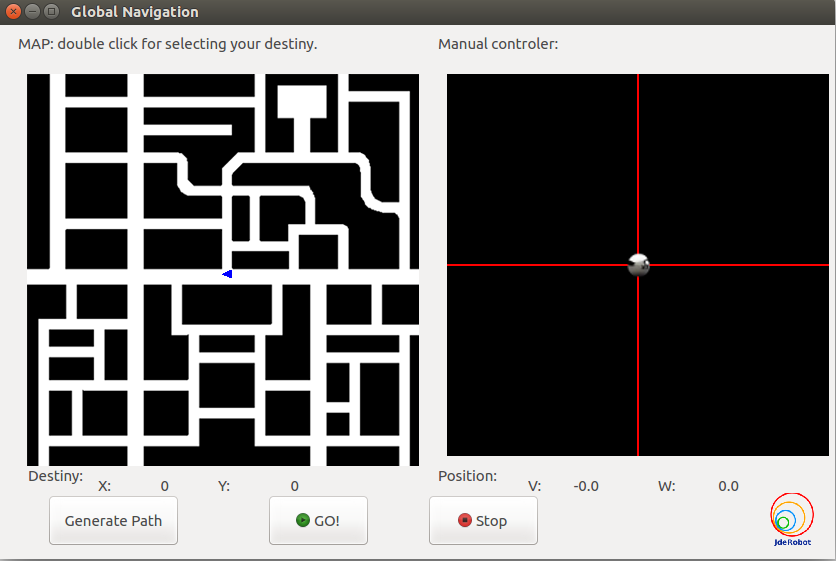
\includegraphics[width=0.5\textwidth]{figures/GPP/GUI_correcta.png}
		\caption{Interfaz gráfica (\acrshort{gui}) actual del \acrshort{gpp}}
		\label{fig.gui_correcta}
		\end{center}
\end{figure}

\begin{figure}[H]
  \begin{center}
    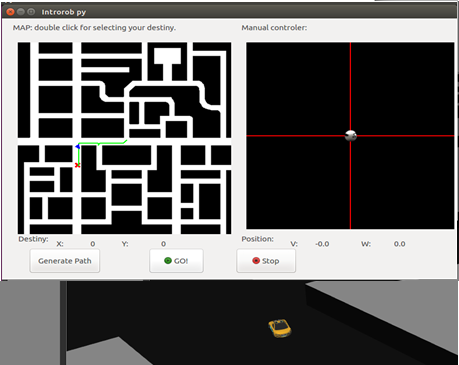
\includegraphics[width=0.5\textwidth]{figures/GPP/triangulo_girado_mal.png}
		\caption{Interfaz gráfica con el triángulo que representa al taxi mal pintado}
		\label{fig.triangulo_girado_mal}
		\end{center}
\end{figure}

\begin{figure}[H]
  \begin{center}
    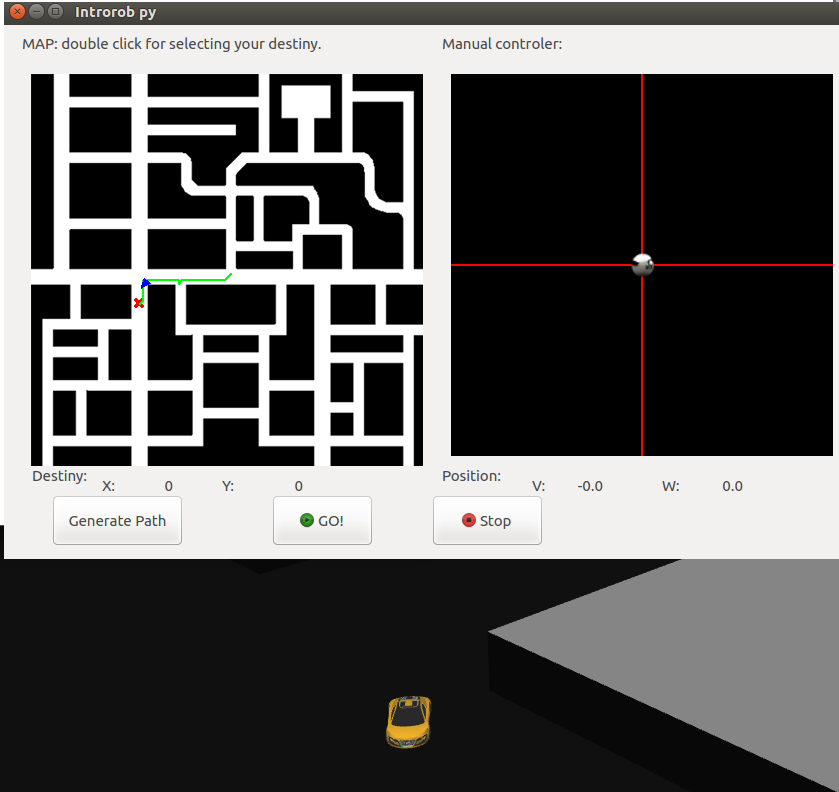
\includegraphics[width=0.5\textwidth]{figures/GPP/triangulo_giro_correcto.png}
		\caption{Interfaz gráfica con el triángulo que representa al taxi correctamente pintado}
		\label{fig.triangulo_giro_correcto}
		\end{center}
\end{figure}

En la interfaz, además se muestra debajo del mapa del mundo la posición numérica exacta que tiene el taxi al iniciarse la práctica en el eje X y en el eje Y. Esta interfaz gráfica (Figura~\ref{fig.gui_correcta}) además muestra un teleoperador a la derecha con el que se puede mover manualmente el taxi en el mundo de Gazebo si se desea.  Por otra parte, debajo del teleoperador podemos ver la velocidad lineal y velocidad angular que tiene al teledirigir el taxi.\\

La \acrshort{gui} posee tres botones, de los cuales dos de ellos serán utilizados para poder ver cómo se lleva a cabo el algoritmo que ha programado el alumno. Cuando pulsamos el botón ``\textit{Generate Path}'', podemos ver el resultado del código que resuelve la parte de la planificación y cómo genera en la imagen del mapa una ruta. De ser pulsado el botón ``\textit{GO!}'' se activará la parte de código que ejecuta el pilotaje del taxi, y podremos ver cómo nuestro taxi navega por las carreteras de la ciudad. El tercer botón sirve para cuando estamos empleando el teleoperador. Este botón nos permitirá parar el taxi si queremos.\\

Se ha modificado el tamaño del visor de la imagen que muestra la \acrshort{gui}, ya que antiguamente no se podía ver la parte inferior del mapa en la \acrshort{gui}, por lo que existían puntos de la carretera a los que no podíamos ir. En las siguientes imágenes se puede comprobar la diferencia que acabamos de mencionar entre la antigua \acrshort{gui} y la actual:
\begin{figure}[H]
  \begin{center}
    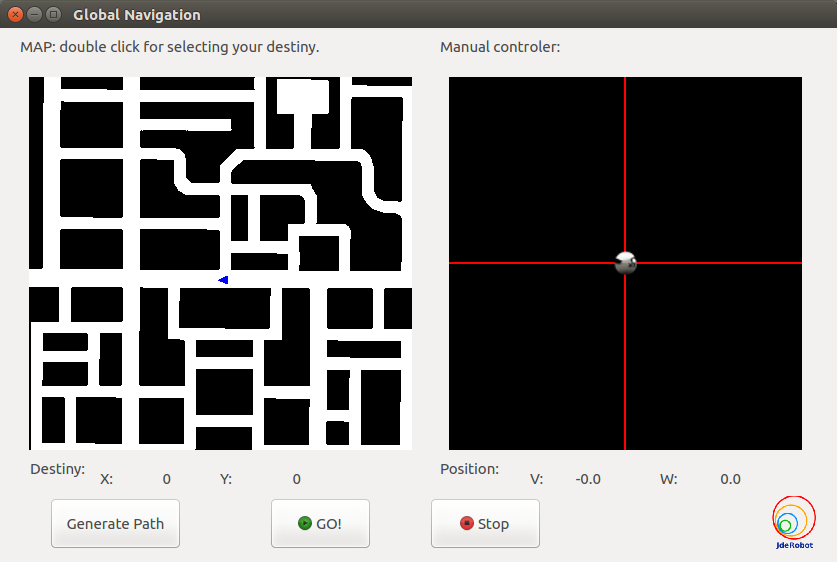
\includegraphics[width=0.5\textwidth]{figures/GPP/GUI_mal.png}
		\caption{Interfaz gráfica (\acrshort{gui}) antigua del \acrshort{gpp}}
		\label{fig.gui_mal}
		\end{center}
\end{figure}

\subsection{Código auxiliar: Clase Grid}
Dentro del componente académico la clase \textit{Grid} se creó en la anterior versión de ``TeleTaxi'', pero se han modificado algunos aspectos en esta versión. Esta clase ofrece un mapa que ayuda al programador a resolver la práctica, permite manipular el mapa de ocupación, crear la rejilla que se emplea para el cálculo del campo y permite controlar la variable ``destino de navegación''.\\

Este componente académico es el que se encarga de capturar información del mundo, crear una rejilla donde se almacenará el campo de la expansión y comunicarse con la interfaz gráfica. Este componente será lanzado al ejecutar la práctica y lanzar la \acrshort{gui}.\\

La clase (\textit{Grid}) será instanciada en el programa principal (\textit{globalNavigation.py}). Cuando es lanzado este componente, se crea una rejilla del tamaño de la imagen del mapa que tiene la interfaz gráfica (400 x 400 píxeles). Esta rejilla se crea para guardar información acerca del mundo. Será utilizada por el alumno para guardar los valores del campo del gradiente (será explicado en el punto~\ref{sec.solucion}) y ayudará a realizar el pilotaje del robot. Además, se inicializa otra rejilla, llamada \textit{path} para almacenar la ruta más corta, la cual se pintará en verde sobre el mapa.\\

Al ejecutar la práctica también se inicializa la variable \textit{map}. Esta variable se inicializa desde la interfaz gráfica y es una imagen binaria del mundo. Tiene representados en negro (valor 0) los píxeles que forman parte de los obstáculos, mientras que los píxeles que forman parte de la carretera serán blancos (valor 255). La imagen será de tres canales, aunque para la solución de la práctica bastará con usar un canal. Este mapa ayudará al alumno a realizar la solución, ya que se puede extraer mucha información de la misma. Esta imagen del mapa ha sido cambiada en la versión actual, debido a que la anterior estaba algo torcida y faltaba una parte del mapa en la parte inferior. Se puede ver en la Figura~\ref{fig.imag_mapa} la diferencia entre la imagen antigua y la actual.

\begin{figure}[H]
  \begin{center}
    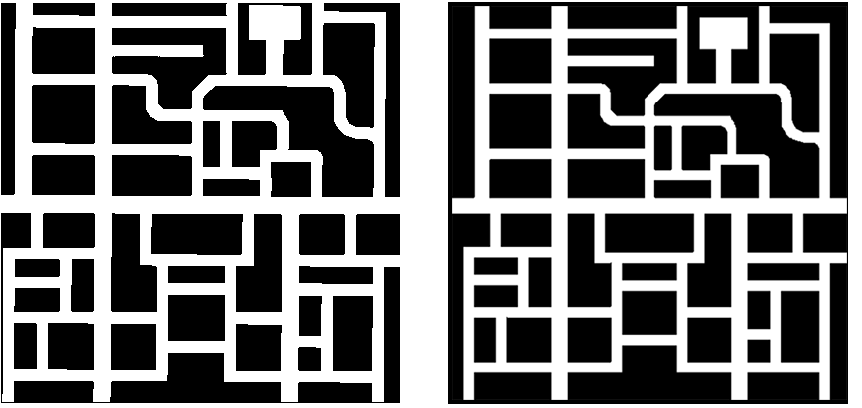
\includegraphics[width=0.8\textwidth]{figures/GPP/imagenes_Mapa.png}
		\caption{Imagen antigua(izquierda) del mapa e imagen actual (derecha)}
		\label{fig.imag_mapa}
		\end{center}
\end{figure}

Este objeto posee una función (llamada \textit{setDestiny}) que será despertada una vez hagamos click sobre la interfaz gráfica para seleccionar el destino deseado. Esta función almacenará las coordenadas del destino en una variable (\textit{destiny}). Esta variable será de gran utilidad para la resolución de la práctica.\\

El objeto \textit{Grid} cuenta con funciones que le permiten relacionarse con el mapa del mundo:

\begin{itemize}
\item \textit{grid.getMap()}: devuelve la imagen del mapa que se está mostrando.
\item \textit{grid.getDestiny()}: devuelve el destino seleccionado en la interfaz gráfica. Este destino se devuelve como una tupla (x, y).
\item	\textit{grid.getPose()}: devuelve la posición respecto al mapa. También será una tupla (x, y).
\item	\textit{grid. showGrid()}: crea una ventana en la que representa los valores del campo que se le han asignado a la rejilla. Los valores más pequeños del campo tendrán un color más cercano a negro, y se irán haciendo más claros a medida que se trate de valores superiores. 
 
\end{itemize}

Este objeto \textit{Grid} también posee funciones que permiten interactuar con la rejilla del campo ficticio (donde se apunta la distancia al destino en ella). Los valores de esta rejilla son de tipo float.  Las funciones son:

\begin{itemize}
\item	\textit{grid.setVal(x, y, val)}: Esta función establece el valor val en la posición indicada (x, y).
\item	\textit{grid.getVal(x, y)}: devuelve el valor de la posición (x, y) del \textit{grid}.
\end{itemize}

El objeto \textit{Grid} consta de funciones que interactúan con la rejilla que contiene la ruta más corta. Los puntos de la rejilla con valor 0 serán ignorados, mientras que los valores superiores a 0 serán considerados parte del camino. Las funciones para interactuar con esta rejilla son:

\begin{itemize}
\item\textit{ grid.setPathVal(x,y, val)}: establece el valor val en la posición indicada (x, y).
\item	\textit{grid.getPathVal(x,y)}: devuelve el valor de la posición indicada (x, y).
\item \textit{grid.setPathFinded()}: indica que se ha encontrado el camino para que empiece a pintarse.
\end{itemize}

Además, esta clase tiene funciones para pasar de coordenadas del mundo a coordenadas del mapa (fila-columna de la rejilla) y viceversa:

\begin{itemize}
\item \textit{gridToWorld(gridX, gridY)}: recibe las coordenadas x e y del mapa \textit{(gridX, gridY)} y devuelve una tupla con las coordenadas equivalentes en el mundo \textit{(worldX, worldY)}.
\item \textit{worldToGrid(worldX, worldY)}: recibe las coordenadas x e y del mundo \textit{(worldX, worldY)} y devuelve una tupla con las coordenadas equivalentes en el mapa \textit{(gridX, gridY)}.

\end{itemize}

Las funciones \textit{gridToWorld} y \textit{worldToGrid} han sido modificadas en la versión actual, puesto que estas funciones tenían un sistema de conversión muy ``ad hoc'' apropiado para cómo estaba hecha la práctica anteriormente, pero no era genérico. Empleaba un sistema de conversión por casos, en vez de emplear matrices de rotación y traslación para pasar de un sistema de referencia a otro. Por eso se ha modificado empleando estas matrices. Uno de los motivos del cambio fue que no era correcta la conversión, sino que era aproximada, lo que provocaba una desviación que afectaba al sistema de pilotaje. Si por ejemplo, teníamos una ruta pintada por el centro de la carretera en la \acrshort{gui}, al realizar el cambio a coordenadas del mundo nos daba como resultado una posición de Gazebo con la cual el coche iba pegado a las paredes, y por ello se chocaba con ellas. En la Figura~\ref{fig.centros} podemos ver la imagen del mapa con la antigua versión (a la izquierda) y la misma con la nueva versión (a la derecha). En este mapa se ha pintado un píxel en rojo en la posición (200, 200), que corresponde con el centro de la imagen, y con la posición donde se encuentra el taxi al lanzar la práctica. 

\begin{figure}[H]
  \begin{center}
    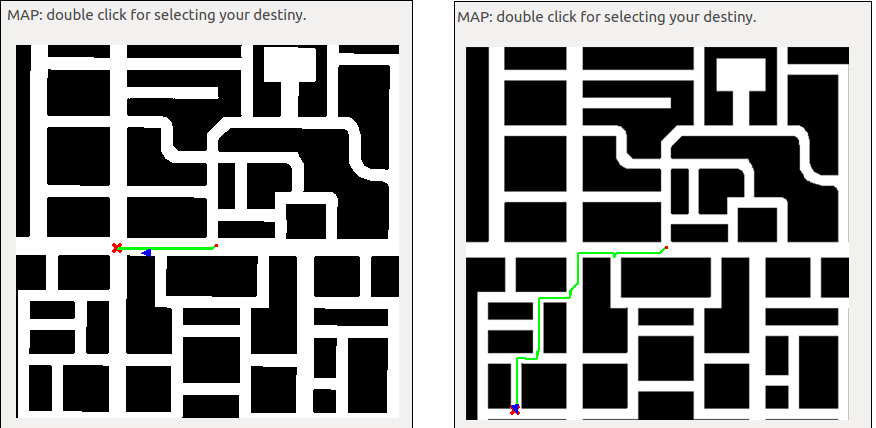
\includegraphics[width=0.8\textwidth]{figures/GPP/centros.png}
		\caption{Imágenes con el centro incorrecto (izquierda) y el centro correcto (derecha)}
		\label{fig.centros}
		\end{center}
\end{figure}

Las matrices de rotación y traslación son muy útiles para pasar de un sistema de referencia del mundo en 3D a un sistema de referencia del mapa en 2D o, al contrario. Estos cambios de sistema de referencia son necesarios porque en la práctica si realizamos la expansión del campo del gradiente sobre una rejilla debemos saber la relación entre cada celdilla de la rejilla con el mundo. Los sistemas de referencia de cada sistema están situados de la siguiente forma:

\begin{figure}[H]
  \begin{center}
    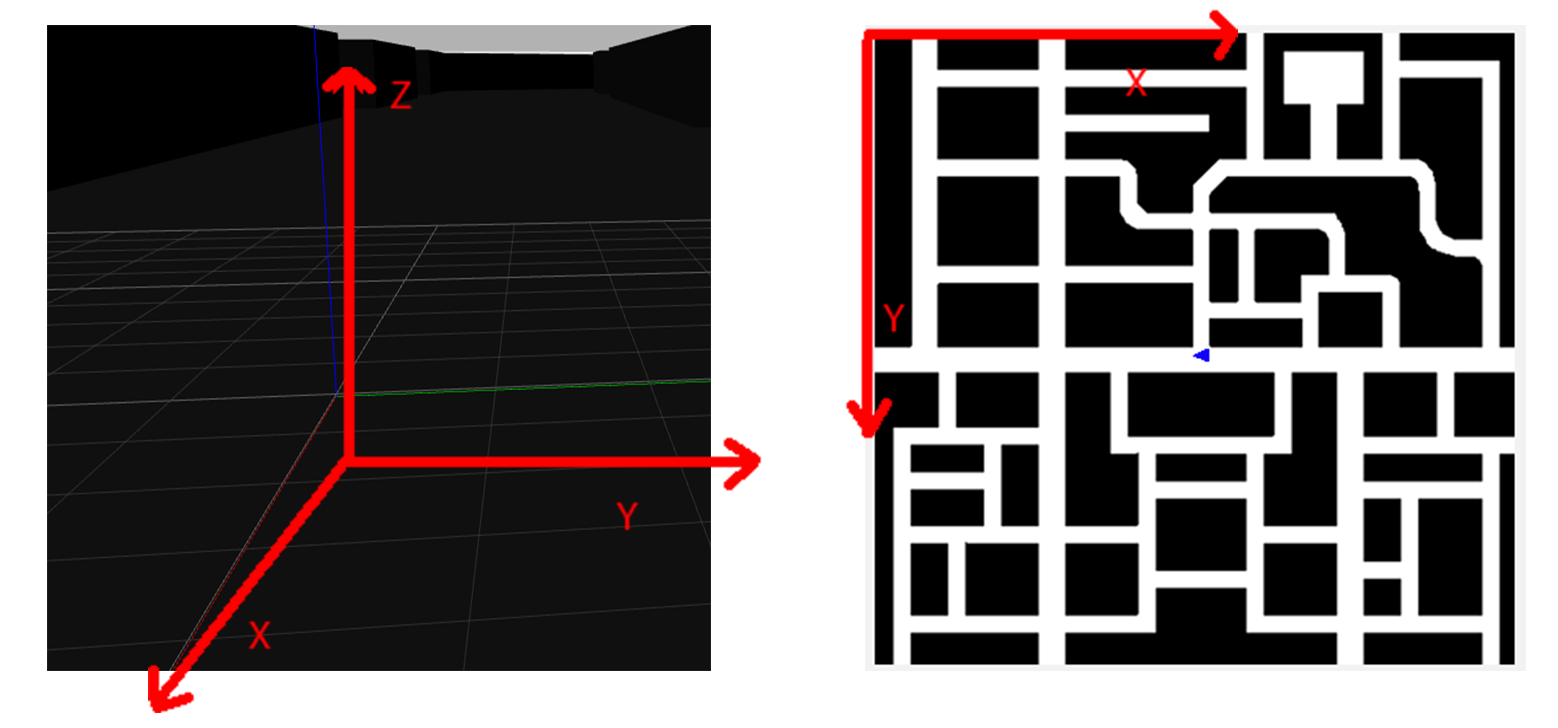
\includegraphics[width=0.8\textwidth]{figures/GPP/referencias.png}
		\caption{Sistema de referencia del mundo (izquierda) y sistema de referencia del mapa (derecha)}
		\label{fig.sistemaref}
		\end{center}
\end{figure}

Para pasar de un sistema a otro deberemos aplicar la rotación y la traslación necesarias. Por ejemplo, en la función \textit{WorldGrid} tenemos que pasar de una coordenada (x, y, z) en un mundo 3D a una coordenada (x’, y’) en 2D. Primero se aplicará una matriz de rotación de \(\pi\) grados sobre el eje x para que el sistema de coordenadas del mundo rote de la siguiente forma:

\begin{figure}[H]
  \begin{center}
    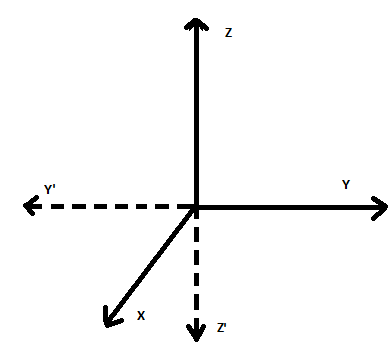
\includegraphics[width=0.4\textwidth]{figures/GPP/Sistema3DRot.png}
		\caption{Rotación sobre el sistema de referencia del mundo (sistema punteado)}
		\label{fig.sistema3DRot}
		\end{center}
\end{figure}

Por si tenemos que aplicar alguna traslación además de la rotación, tenemos una matriz de rotación y traslación para el eje x. Si no queremos realizar una traslación los puntos tx, ty, y tz tendrán valor 0. La traslación se debe a que queremos tener el punto (0,0) de la imagen en la esquina superior izquierda. El cambio lo realizamos siguiendo la ecuación~\ref{ec.matriz}.

\begin{equation}
\label{ec.matriz}
\left[\begin{array}{cc}
x' \\ 
y' \\
z' \\
1
\end{array}\right] = \left[\begin{array}{cccc}
1 & 0 & 0 & tx \\ 
0 & \cos(\alpha) & -\sin(\alpha) & ty\\
0 & \sin(\alpha) & \cos(\alpha) & tz \\
0 & 0 & 0 & 1
\end{array}\right]* \left[\begin{array}{cc}
x \\ 
y \\
z \\
1
\end{array}\right]
\end{equation}
 
Lo siguiente que tendremos que hacer es aplicar una rotación de –\(\pi\)/2 grados sobre el eje z y una traslación si los puntos están un poco desviados. La traslación será de 200 píxeles (ancho de la imagen/2) en x y -200 píxeles (-alto de la imagen/2) en y. Por lo tanto, tx será en este caso 200, y ty será -200, tz será 0. La matriz de rotación y traslación la aplicamos de la siguiente forma:

\begin{equation}
\left[\begin{array}{cc}
x' \\ 
y' \\
z' \\
1
\end{array}\right] = \left[\begin{array}{cccc}
\cos(\alpha) & -\sin(\alpha) & 0 & tx \\ 
\sin(\alpha) & \cos(\alpha) & 0 & ty\\
0 & 0 & 1 & tz \\
0 & 0 & 0 & 1
\end{array}\right]* \left[\begin{array}{cc}
x \\ 
y \\
z \\
1
\end{array}\right]
\end{equation}

Para realizar la conversión de la imagen al mundo deberemos aplicar las matrices de rotación inversas a estas. 

\section{Solución de Referencia}\label{sec.solucion}
El objetivo de esta práctica es proveer al robot de un algoritmo de navegación, que estará compuesto por un algoritmo de navegación global y otro de pilotaje. El algoritmo de cálculo del campo (navegación global) se realizará en una iteración sin tiempo límite, y el algoritmo de pilotaje responde a un control reactivo. En esta sección abordaremos una breve explicación sobre navegación autónoma de robots, una descripción de la técnica \textit{Gradient Path Planning}, y la solución concreta de la práctica. El fichero \textit{MyAlgorithm.py} donde se inserta el código de la solución de referencia es de naturaleza iterativa, ejecuta continuamente iteraciones y en cada una de ellas se percibe y se controla. El alumno tiene que rellenar con su código la función \textit{execute}, que el componente académico invoca periódicamente.

\subsection{Fundamentos de la Navegación global y el algoritmo GPP}
El principal problema de los robots móviles es la navegación autónoma. Es la capacidad que poseen los robots para ir desde un punto del espacio a otro cualquiera evitando chocarse con algún obstáculo, ya sean objetos fijos u objetos móviles inesperados. Esta es una tarea compleja, que provee a los robots de grandes capacidades. La navegación de los robots de forma habitual se divide en dos ramas: la navegación global y la navegación local.\\

La navegación global consiste en calcular o planificar una ruta de forma óptima inicialmente para que el robot la pueda seguir. Para llevar a cabo este proceso el robot debe tener un conocimiento previo del escenario por el cual se debe mover. El robot suele tener previamente esta información mediante un mapa del entorno. De no ser así, el robot adquirirá dicho conocimiento construyendo un mapa del entorno por medio de los sensores que posee. La ruta se construye empleando técnicas de búsqueda o planificación, que requieren un tiempo considerable. Ejemplos de estas técnicas son: grafos de visibilidad y \textit{Gradient Path Planning}.\\

Para solucionar el problema de la navegación global, hemos escogido el algoritmo \textit{Gradient Path Planning} (\acrshort{gpp}), que garantiza una trayectoria mínima entre el punto desde el que partimos hasta el punto de destino. La trayectoria calculada no se basa en la distancia euclídea mínima, sino que se incorporan los obstáculos en el cálculo de la trayectoria.\\

Para desarrollar el algoritmo \textit{Gradient Path Planning} hemos partido del trabajo desarrollado por Kurt Konolige~\cite{gradient}, así como de trabajos previos realizados en la Universidad Rey Juan Carlos~\cite{navegacion_autolocalizacion3}~\cite{navegacion_autolocalizacion4}. Esta técnica obtiene el camino óptimo desde el punto de partida hasta el destino.\\

La técnica \acrshort{gpp} consiste en generar un frente de onda circular que parte desde la posición de destino, y que recorre el espacio libre del mapa hasta llegar a la posición de partida del robot. El punto donde está situado el robot es el comienzo de la ruta que recorrerá el robot. En su propagación, el frente de onda asignará valores de forma creciente a cada punto libre del espacio por el que pase. Antes de comenzar la propagación del frente de onda, todos los puntos libres del espacio tienen valor 0. El frente de onda se puede expandir por todo el espacio, hasta la posición que ocupa el robot o un poco más allá.\\

Adicionalmente los obstáculos generarán su propio frente de onda de penalización, lo que implica que los puntos del espacio que estén próximos a los obstáculos aumentarán su valor por defecto considerablemente. El frente de onda de penalización se propaga de forma inversa al frente de onda anterior. Esto quiere decir que los puntos del espacio más próximos a los obstáculos tendrán un valor mayor a los puntos más alejados. El frente de onda de los obstáculos se expande hasta una distancia determinada, no se expanden por todo el espacio.\\

Sumar la expansión del frente de onda de penalización evita que el robot se acerque a los obstáculos al navegar por el espacio. De no ser así, la ruta más corta estaría pegada a los obstáculos, y de esta forma el robot rozaría con las paredes. Esto hará que el robot tenga mayor seguridad.\\

Una vez se ha generado el campo total, el robot podrá navegar hasta el destino evaluando en cada iteración los puntos de su alrededor. Siempre se dirigirá hacia el punto de menor valor del campo calculado. A medida que avance el robot hacia su destino, el campo calculado tendrá menor valor, pues las zonas más próximas al destino son las que menor valor poseen.  \\

El método \acrshort{gpp} permite generar una ruta ideal desde el punto de partida del robot hasta el destino deseado. Esta ruta se generará siguiendo el gradiente del campo calculado, y será la de menor distancia incorporando los obstáculos. Esta técnica de navegación global asegura que llegaremos al objetivo. Sin embargo, es posible que el robot durante el pilotaje no siga exactamente la ruta calculada, pues puede tener desviaciones debidas a la velocidad y rotación del robot. El pilotaje se llevará a cabo de forma reactiva, mirando en cada momento cuál es la celdilla vecina de menor valor a la que debe dirigirse, y si se encuentra próximo a algún obstáculo.\\

La forma reactiva se basa en el ``ahora'', es decir, en cada instante de tiempo evalúa la situación y actúa. No desarrolla una solución inicial y la sigue, sino que va actuando en función de lo que ocurra en cada momento.

\subsection{Construcción del mapa del gradiente}
La navegación global mediante \textit{Gradient Path Planning} se puede implementar de diversas formas. La solución implementada  se desarrolla en el fichero \textit{``MyAlgorithm.py''}. En este fichero podremos observar que la solución se divide en un método en el que se construye el mapa del gradiente, y otro método que se corresponde con el pilotaje del robot.\\

En el método \textit{``generatePath''} del fichero \textit{``MyAlgorithm.py''} llevaremos a cabo el desarrollo del algoritmo que genera el mapa del campo del gradiente. Esta función se ejecutará solamente cuando pulsemos el botón \textit{``Generate Path''} en la \acrshort{gui} (Figura~\ref{fig.gui_correcta}). El escenario estará representado gráficamente por una rejilla, donde iremos almacenando el campo calculado. Esta rejilla es proporcionada por la clase \textit{Grid}.\\

Lo primero que debemos conocer antes de comenzar a generar el campo y expandirlo por la rejilla es el mapa, la posición inicial del robot y la posición de destino deseado. En la práctica, se dispone de un objeto \textit{grid} que permite obtener el mapa a través de la función \textit{grid.getMap()}. Este mapa proporciona información del escenario mediante sus valores, donde el valor 0 representa a los obstáculos y el valor 255 representa la carretera. El destino podrá conocerse, una vez el usuario haya seleccionado el destino deseado en la \acrshort{gui}, mediante la función \textit{grid.getDestiny()}. Por último, podemos obtener la posición del robot respecto al mapa mediante la función \textit{grid.getPose()}.

\subsubsection{Generación campo ficticio de navegación global}
En la función \textit{``generatePath''} inicialmente tendremos un bucle que realiza la propagación de los frentes de onda. Es decir, no tendremos un único frente de onda, sino que vamos a tener diferentes frentes de onda, los cuales se encuentran en una lista ordenada. \\

El bucle de la propagación de los frentes de onda se ejecutará hasta que se expanda el campo un poco más allá de la posición del taxi. En este caso se expandirá hasta 20 celdillas más allá de la celdilla que ocupa el taxi en la rejilla. Este número podría haber sido mayor o menor, pero en el caso de que fuera mayor la propagación tardaría más tiempo en ejecución. Si el número fuera menor tendríamos menos conocimiento de los alrededores iniciales del robot.\\

El punto de partida del frente de onda inicial es el destino, que es la celdilla de la rejilla que posee la distancia 0. Será nuestro primer nodo que expandirá el frente de onda a sus vecinos. Cada nodo expandirá el valor de la distancia a sus 8 celdillas vecinas. Este valor de distancia asignado a las celdillas vecinas será el valor del nodo (distancia) + 1 o el valor del nodo + 1.4 en las diagonales. Cuando se encuentre un obstáculo, se almacenará la celdilla de dicho obstáculo en un array y no se le asignará ninguna distancia. De esta forma aseguramos tener almacenadas las celdillas que pertenecen al borde de un obstáculo para posteriormente penalizar a las celdillas que se encuentren muy próximas a los obstáculos.\\

Cada nodo va a expandir antes el frente a sus vecinos que se encuentren a una distancia +1, y posteriormente expandirá el frente a sus vecinos que estén en una distancia + 1.4. Por lo que se podría decir que el frente de onda de cada nodo se divide en dos frentes de onda. De esta forma nos aseguramos que el frente de onda sea aproximadamente circular (Figura~\ref{fig.primera_expansion_gpp}).

\begin{figure}[H]
  \begin{center}
    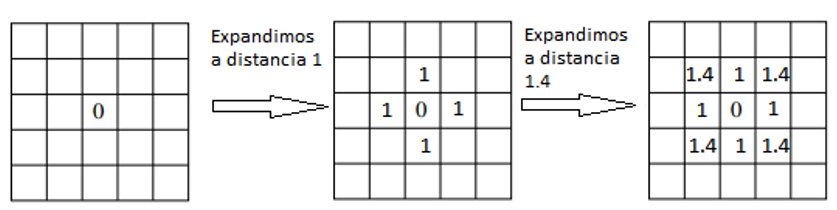
\includegraphics[width=0.8\textwidth]{figures/GPP/primera_expansion.png}
		\caption{Primera propagación del frente de onda}
		\label{fig.primera_expansion_gpp}
		\end{center}
\end{figure}

Este proceso de expansión (Figura~\ref{fig.algoritmo_expansion_gpp}) se irá haciendo sucesivamente hasta llegar a 20 celdillas más alejadas de la posición inicial del taxi. A la hora de realizar la expansión, si las celdillas vecinas tuvieran un valor mayor al que calculara el nodo, dicho valor se actualizaría por el valor que expanda el nodo actual. Esto permite asegurar que siempre tendremos el menor valor posible en cada celdilla.\\

\begin{figure}[H]
  \begin{center}
    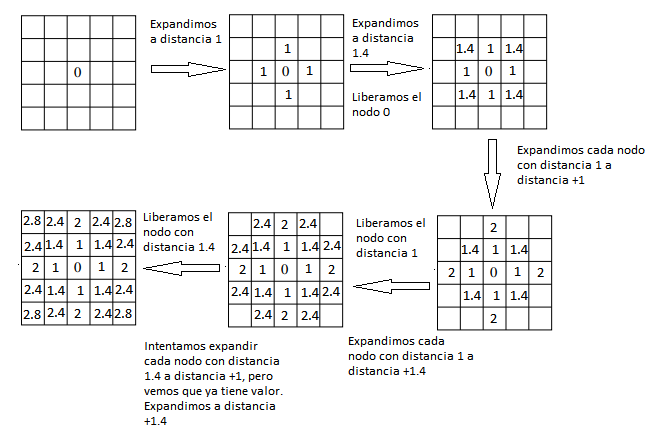
\includegraphics[width=0.8\textwidth]{figures/GPP/algoritmo_expansion.png}
		\caption{Esquema propagación frentes de onda}
		\label{fig.algoritmo_expansion_gpp}
		\end{center}
\end{figure}


En la rejilla del campo que hemos generado (Figura~\ref{fig.expansiones_gpp}) se puede apreciar en color más oscuro los puntos más cercanos al destino, puesto que poseen un valor menor de distancia. Por el contrario, los puntos más lejanos del destino son los que poseerán un color más claro. A continuación, podemos observar una progresión de la expansión del campo.\\

\begin{figure}[H]
  \begin{center}
    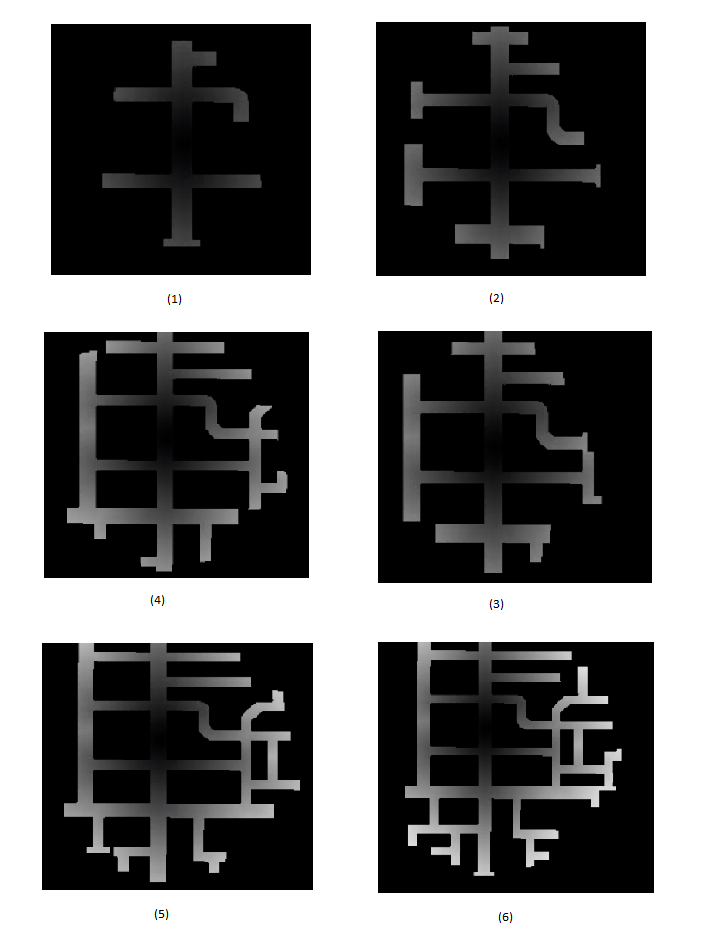
\includegraphics[width=0.8\textwidth]{figures/GPP/expansiones.png}
		\caption{Esquema expansión del campo}
		\label{fig.expansiones_gpp}
		\end{center}
\end{figure}

\subsubsection{Penalización por cercanía de obstáculos}
El segundo paso, es la penalización que realizan los bordes de los obstáculos a las celdillas más próximas. Esta penalización se lleva a cabo para evitar que la ruta más corta desde el robot hasta el destino esté pegada a las paredes de los obstáculos y haga que nuestro taxi roce con las paredes. Con esta penalización nos aseguramos de que en el pilotaje haya un margen de seguridad entre el taxi y las paredes.\\

Como hemos mencionado antes, las celdillas que pertenecen a bordes de obstáculos están almacenadas en un array (llamado \textit{posObstaclesBorder}). Estas celdas (obstáculos) sumarán una penalización a las celdillas vecinas que formen parte de la carretera en función de la distancia a la que se encuentran de la celdilla obstáculo.\\

Para llevar a cabo la penalización por obstáculos se ha creado una nueva rejilla, la cual inicialmente posee un valor 0 en todas sus celdillas. En esta rejilla almacenaremos los valores de penalización. Finalmente sumaremos la rejilla del campo y la de los obstáculos para actualizar sus valores con dichas penalizaciones.\\

La penalización que realizan los obstáculos se llevará a cabo mediante un bucle que recorre el array \textit{posObstaclesBorder}. Cada posición de dicho array penalizará a las celdillas vecinas que están a una distancia de +1, +2 y +3 de la misma. Las celdillas que estén a una distancia de +1 del borde del obstáculo se penalizarán con un valor de 174. Las celdillas con una distancia +2 tendrán una penalización de 168, mientras que las celdillas con una distancia +3 se penalizarán con un valor de 162.\\

En cada penalización que adjuntemos a una celdilla antes comprobaremos su valor en la rejilla de penalización, puesto que dos celdillas del borde del obstáculo pueden querer penalizar a una misma celdilla, pero esta celdilla solamente se puede penalizar una vez. Cuando vayamos a penalizar y comprobemos si ha sido penalizada una celdilla, comprobaremos su valor. Si el valor de penalización que tiene dicha celdilla es menor que el que se iba a añadir, se sustituirá el valor de penalización por el mayor.\\

Estas penalizaciones harán que las celdillas próximas a los obstáculos tengan un valor mayor y aparezcan con un color más claro (blanco) al mostrar el \textit{grid} (Figura~\ref{fig.campos_gpp}). El \textit{grid} lo podemos mostrar mediante la función \textit{grid.showGrid()}. Esta función crea una ventana en la que representa los valores del campo que se le han asignado a la rejilla. Podemos ver en la Figura~\ref{fig.campos_gpp} una serie de ejemplos de diferentes campos calculados con la penalización por obstáculos incluida.\\

\begin{figure}[H]
  \begin{center}
    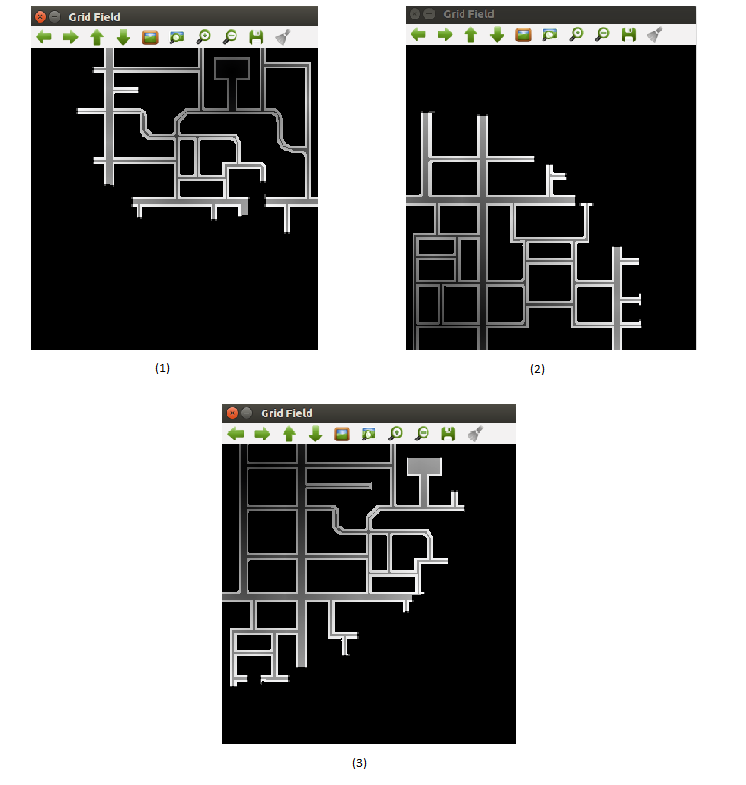
\includegraphics[width=0.8\textwidth]{figures/GPP/campos.png}
		\caption{Representación campos calculados}
		\label{fig.campos_gpp}
		\end{center}
\end{figure}

\subsubsection{Cálculo de ruta ideal}
El paso siguiente es el cálculo de la ruta más corta. Esta ruta se calcula para observar cuál sería la ruta ideal que debe seguir nuestro taxi. Dicha ruta sigue las celdillas de menor valor de distancia.\\


El cálculo de la ruta más corta comienza en la celdilla donde se encuentra situado el taxi y termina al alcanzar la celdilla que posee el valor de distancia 0, es decir, el destino. Para ir almacenando la ruta tenemos que hacer uso de la función \textit{grid.setPathVal}, la cual establece el valor en la posición que se le indica, tomando como ruta las celdillas que poseen un valor diferente a 0. \\

Comenzamos el cálculo de la ruta añadiendo la posición inicial del taxi a la ruta. El siguiente paso es comprobar las celdillas vecinas de la celdilla que ocupa el taxi. Entre estos vecinos añadiremos a la ruta la de menor valor de distancia. Después, comprobaremos los vecinos de esta nueva celdilla y así continuamente hasta llegar a la celdilla destino.\\

Una vez que alcancemos la celdilla del destino tendremos que indicar que hemos terminado de calcular la ruta más corta y que se puede comenzar a pintar. Para ello empleamos la función \textit{grid.setPathFinded}.\\

En la Figura~\ref{fig.rutas_gpp} se pueden observar diferentes rutas calculadas en función del destino que hemos elegido. En las imágenes (1), (2) y (3), podemos ver las rutas calculadas aplicando la penalización de los obstáculos; mientras que en las imágenes (4), (5) y (6) vemos las rutas que se han calculado para los mismos destinos que en (1), (2) y (3), pero sin realizar la penalización de los obstáculos.\\

\begin{figure}[H]
  \begin{center}
    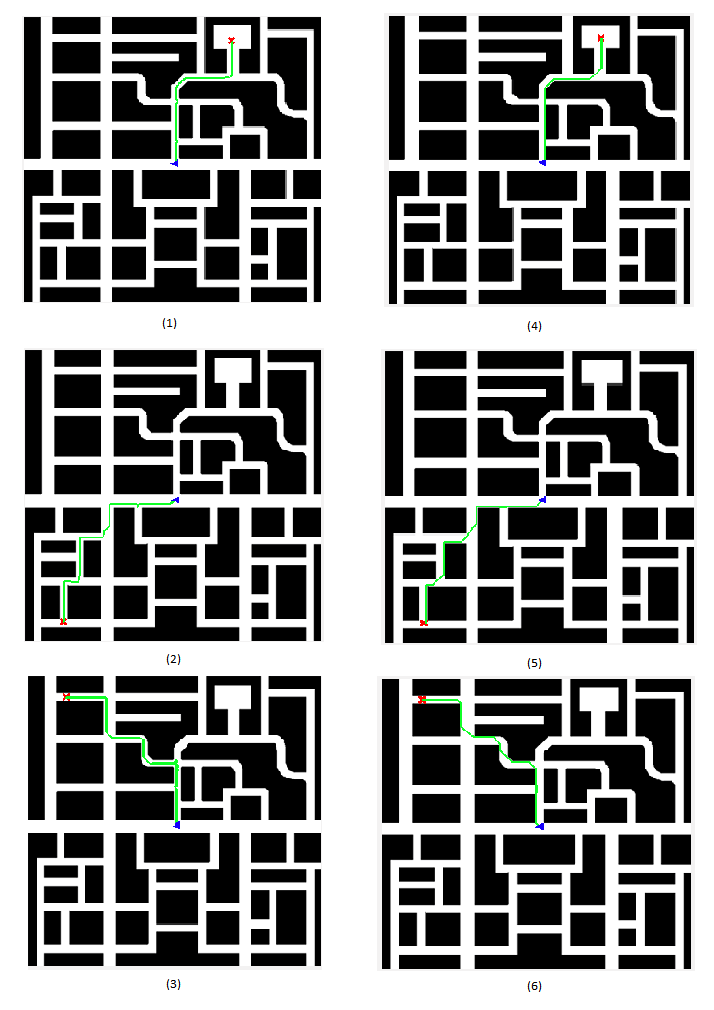
\includegraphics[width=0.8\textwidth]{figures/GPP/rutas.png}
		\caption{Esquema expansión del campo}
		\label{fig.rutas_gpp}
		\end{center}
\end{figure}

\subsection{Pilotaje del robot}\label{sec.pilotaje}
En el método \textit{``execute''} del fichero \textit{``MyAlgorithm.py''} incluimos el código del algoritmo correspondiente al pilotaje del taxi. Este método se ejecuta periódicamente para que el pilotaje sea un control reactivo.\\

Este algoritmo se encarga de pilotar el robot desde su posición inicial hasta la posición del destino mediante el campo calculado en el método \textit{generatePath}. La dificultad está en la elección de la velocidad de tracción y la velocidad de rotación que debemos ordenar al taxi. \\

El pilotaje se ha realizado sin tener en cuenta la ruta más corta calculada en el punto anterior, ya que dicha ruta es el ideal a seguir, pero el taxi al seguir órdenes de velocidad de tracción y de rotación puede desviarse un poco de dicha ruta. Si intentara seguir la ruta ideal estrictamente, el taxi realizaría movimientos muy forzados hasta llegar al destino. Lo ideal es que el taxi se mueva de una forma suave, como lo haría un taxi real. En el pilotaje se ha tenido en cuenta el campo calculado. De esta forma, en cada iteración el taxi irá comprobando el valor de distancia de las celdillas que se encuentran en un cierto radio de distancia con respecto a su posición. De estas celdillas elegirá como objetivo la celdilla de menor valor. Este planteamiento permite que el taxi tenga un comportamiento reactivo ante imprevistos y que se asemeje un poco a la navegación local, ya que no tiene en cuenta únicamente la ruta más corta calculada previamente, también tiene en cuenta la situación del taxi.\\

Inicialmente en el pilotaje debemos comprobar la pose de nuestro taxi mediante el sensor de posición y la posición del destino para ver cuál es la situación del taxi, ya que si el taxi ha alcanzado el destino debe detenerse. Conocemos la celdilla que ocupa el destino en el \textit{grid}, pero el sensor de posición devuelve la posición del taxi con respecto al mundo. Esto implica que debemos convertir las coordenadas del destino en el \textit{grid} en coordenadas respecto al mundo para comprobar si hemos llegado a dicho destino. Para ello se usa la función (\textit{grid.gridToWorld}) que realiza la correspondencia de las coordenadas del \textit{grid} con la posición que tendrían estas coordenadas en el mundo de Gazebo.\\

El siguiente paso es calcular el objetivo local próximo al robot. Vamos a ir calculando en cada iteración un objetivo que se encuentra a cierto radio de distancia del robot. Comprobando los valores de distancia del campo que habíamos calculado en el punto anterior. Por lo que tendremos que obtener la posición del taxi en el sistema de coordenadas del \textit{grid} (mediante la función \textit{worldToGrid}). En nuestro caso comprobaremos las celdillas situadas a una distancia de 5 celdillas con respecto a la posición del robot y escogeremos la de menor valor como objetivo local. El objetivo no es exactamente el anterior mencionado, sino que vamos a calcular un segundo objetivo situado a 5 celdillas del primer objetivo, y posteriormente haremos la interpolación de estos dos objetivos obteniendo el objetivo final al que queremos llegar. El motivo de esta interpolación y ese cálculo doble es obtener un pilotaje con movimientos más suaves. Además, esto nos permite que el taxi gire adecuadamente en las curvas. \\

El objetivo local final calculado está en coordenadas del \textit{grid}, por lo que tendremos que hacer un cambio de coordenadas relativas al mundo para obtener el objetivo en coordenadas del mundo. Una vez lo tengamos, podremos calcular el vector de dirección que tendrá nuestro robot para llegar hasta este y el ángulo. Para ello debemos tener en cuenta la pose que nos devuelve el sensor de posición, así como la orientación del robot (en radianes), las cuales están en coordenadas absolutas del mundo.\\

En esta práctica hay dos sistemas de referencia. Por un lado, tenemos el sistema de referencia absoluto, en el cual se pueden representar la posición del robot y la de cualquier otro objeto. En nuestro caso serán los ejes de Gazebo, por lo cual el punto fijo de referencia será el punto de coordenadas (0, 0, 0) en el mundo de Gazebo. El otro sistema de referencia que vamos a tener en cuenta es el sistema de referencia solidario con el robot. Según se mueva el taxi este sistema de referencia solidario con el robot se desplazará. También hay que mencionar que inicialmente el robot comienza con una rotación de –\(\pi\)/2 radianes.\\

En la Figura~\ref{fig.sistemaReferencia_gpp} podemos ver el sistema de referencia absoluto (son los ejes finos azul, verde y rojo que atraviesan la imagen) y el sistema de referencia solidario con el robot (flechas gruesas azul, roja y verde que salen del robot):

\begin{figure}[H]
  \begin{center}
    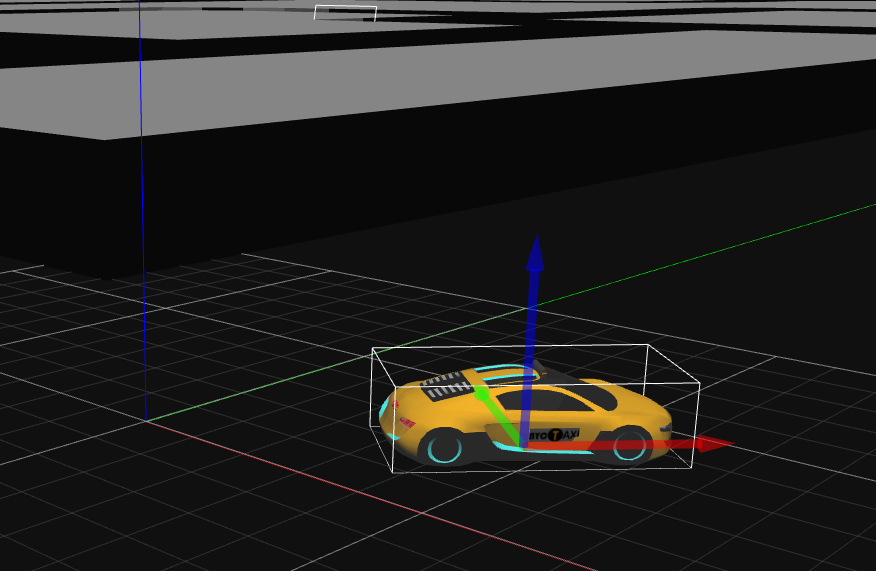
\includegraphics[width=0.5\textwidth]{figures/GPP/sistemaReferencia_GPP.png}
		\caption{Sistema de referencia absoluto (Gazebo) y sistema de referencia solidario con el robot}
		\label{fig.sistemaReferencia_gpp}
		\end{center}
\end{figure}

Se ha decidido definir el sistema de referencia solidario con el robot de la siguiente forma: el eje X de este sistema es el que señala al frente del robot, mientras que el eje Y es el que señala a la izquierda del robot. El origen de este sistema es un punto situado en el centro geométrico del robot.

\begin{figure}[H]
  \begin{center}
    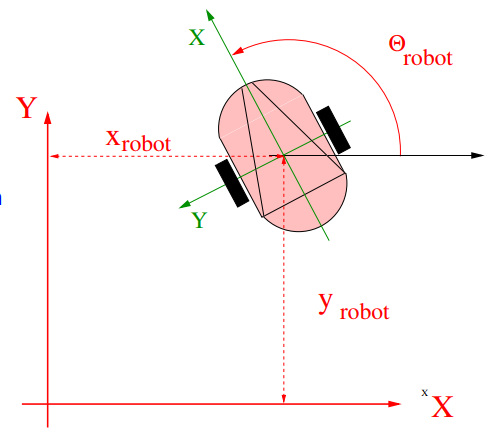
\includegraphics[width=0.5\textwidth]{figures/GPP/sistemasReferencia.png}
		\caption{Sistema de referencia absoluto y sistema de referencia solidario con el robot}
		\label{fig.sistemasReferencia_gpp}
		\end{center}
\end{figure}

El sistema de referencia solidario con el robot se emplea para expresar las coordenadas relativas de los objetivos próximos o de obstáculos respecto al robot. Si tenemos un punto P que no se mueve en el espacio para el sistema de referencia absoluto no habrá movimiento, pero para el sistema de referencia solidario con el robot las coordenadas de este punto P varían.\\

Sabiendo las coordenadas absolutas de un punto, y las coordenadas absolutas del robot y su orientación, podemos pasar las coordenadas absolutas a relativas o al revés. En nuestro caso deberemos pasar las coordenadas absolutas de cada objetivo próximo a coordenadas relativas al sistema del robot para calcular la velocidad de tracción y rotación que debe tener el taxi.\\

Con la transformación de coordenadas absolutas a relativas obtenemos un vector de dirección, con el que podremos calcular el ángulo que hay entre el origen del sistema relativo al robot y la posición relativa del objetivo local. Para obtener el vector de dirección hemos creado una función, en la que primero calcularemos la diferencia entre las coordenadas absolutas del objetivo y las coordenadas absolutas del robot (dx, dy), y después a esta diferencia le aplicamos una matriz de rotación para obtener el vector de dirección. En esta matriz de rotación tendremos en cuenta la orientación  (\(\Theta\)) del robot.

\begin{equation} 
x' = dx \cos(\Theta) - dy \sin(\Theta)
\end{equation}

\begin{equation} 
y' = dx \sin(\Theta) - dy \cos(\Theta)
\end{equation}


Con este vector de dirección conocemos dónde se encuentra situado el punto objetivo con respecto a nuestro origen del sistema del robot, ahora podremos calcular el ángulo que debe rotar el robot para alinearse con este punto. Este ángulo lo calcularemos mediante el cálculo del arco tangente. En la Figura~\ref{fig.Triangulo_gpp} podemos ver un dibujo del ángulo \(\alpha\) que queremos calcular y el punto P (objetivo). Conociendo estos datos podemos calcular \(\alpha\) con la arco tangente.

\begin{figure}[H]
  \begin{center}
    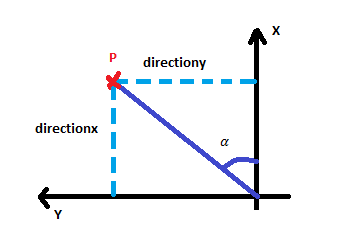
\includegraphics[width=0.5\textwidth]{figures/GPP/Triangulo.png}
		\caption{Sistema de referencia solidario con el robot y punto objetivo}
		\label{fig.Triangulo_gpp}
		\end{center}
\end{figure}

El ángulo \(\alpha\) lo podemos calcular de la siguiente forma:

\begin{equation} 
\alpha = arcotang\left(\frac{directiony}{directionx}\right)
\end{equation}

El ángulo calculado \(\alpha\) está en radianes. Si este ángulo es muy grande significará que debemos dotar al taxi de una velocidad de rotación alta. Por el contrario, si este ángulo es muy pequeño significa que el robot se encuentra más o menos alineado con el objetivo y que probablemente la velocidad de rotación de nuestro vehículo sea 0.\\

En esta solución se ha realizado un control por casos en función del ángulo \(\alpha\)  calculado. En función de este ángulo ordenaremos al taxi mayor o menor velocidad de tracción y de rotación en esa iteración de control. Si el ángulo calculado es muy elevado aplicaremos una velocidad de tracción reducida y una velocidad de rotación elevada (el coche puede estar en una curva o necesitar realizar un gran giro). Sin embargo, si el ángulo es pequeño, le daremos al taxi una velocidad de tracción elevada (ya que se encuentra en una recta) y poca velocidad de rotación.\\

En las Figuras~\ref{fig.camino1_G_gpp},~\ref{fig.camino2_G_gpp},~\ref{fig.camino3_G_gpp} y~\ref{fig.camino4_G_gpp} podemos observar una secuencia de imágenes en la que se ha calculado una ruta y podemos ver cómo aproximadamente el taxi sigue esta ruta, pero a veces se desvía un poco, como habíamos mencionado anteriormente que podría suceder. El taxi alcanza el destino deseado con éxito.

\begin{figure}[H]
  \begin{center}
    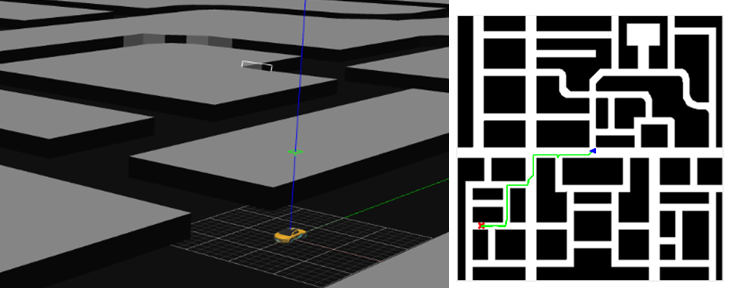
\includegraphics[width=0.8\textwidth]{figures/GPP/camino1_G.png}
		\caption{Posición 1 taxi en el mundo de Gazebo y en la \acrshort{gui}}
		\label{fig.camino1_G_gpp}
		\end{center}
\end{figure}

\begin{figure}[H]
  \begin{center}
    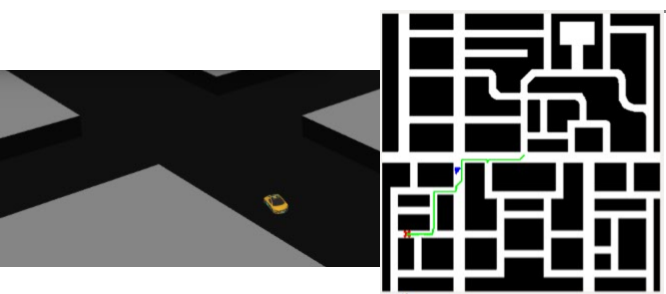
\includegraphics[width=0.8\textwidth]{figures/GPP/camino2_G.png}
		\caption{Posición 2 taxi en el mundo de Gazebo y en la \acrshort{gui}}
		\label{fig.camino2_G_gpp}
		\end{center}
\end{figure}

\begin{figure}[H]
  \begin{center}
    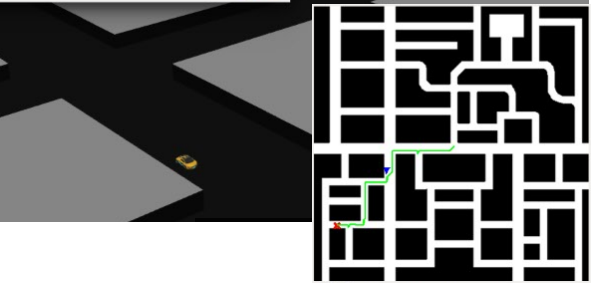
\includegraphics[width=0.8\textwidth]{figures/GPP/camino3_G.png}
		\caption{Posición 3 taxi en el mundo de Gazebo y en la \acrshort{gui}}
		\label{fig.camino3_G_gpp}
		\end{center}
\end{figure}

\begin{figure}[H]
  \begin{center}
    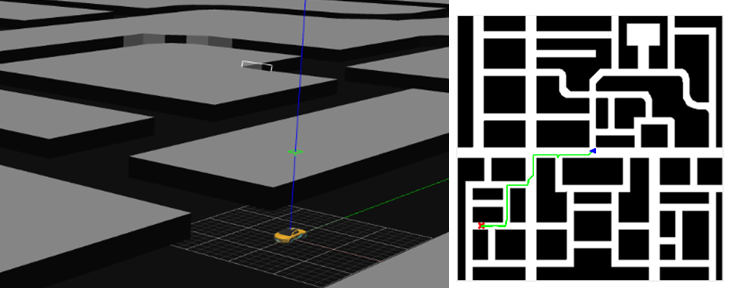
\includegraphics[width=0.8\textwidth]{figures/GPP/camino1_G.png}
		\caption{Posición 4 (destino) taxi en el mundo de Gazebo y en la \acrshort{gui}}
		\label{fig.camino4_G_gpp}
		\end{center}
\end{figure}

\section{Evaluador Automático}
La práctica consta además de un evaluador automático que tiene en cuenta ciertos parámetros para calificar el algoritmo que programa el alumno. Este evaluador automático tiene una interfaz gráfica que muestra los diferentes parámetros, así como la nota final. Para crear el evaluador automático se ha empleado PyQt5 y se han creado clases diferentes para cada parámetro que queramos mostrar. Estas clases serán instanciadas en una clase principal llamada \textit{MainWindowReferee}, que contiene la ventana principal del evaluador automático.\\

\begin{figure}[H]
  \begin{center}
    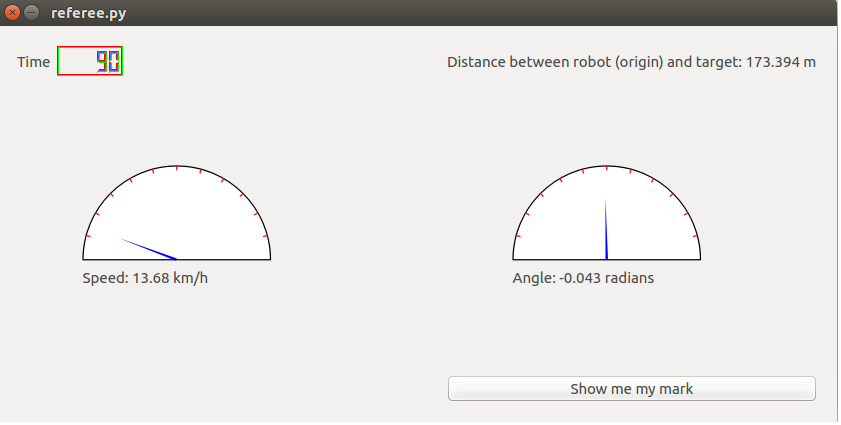
\includegraphics[width=0.7\textwidth]{figures/GPP/referee2_gpp.png}
		\caption{Evaluador Automático del \acrshort{gpp} durante el pilotaje}
		\label{fig.referee2_gpp}
		\end{center}
\end{figure}

El evaluador (Figura~\ref{fig.referee2_gpp}) tiene en su visor un reloj digital que va mostrando los segundos que han pasado desde que se arrancó la práctica. Este visor de tiempo está programado en una clase (llamada \textit{timeWidget}), en la cual se almacenará en una variable los segundos que el taxi está realizando el pilotaje.\\

En segundo lugar, se ha creado una clase (\textit{distanceWidget}) para mostrar la distancia euclídea que existe entre la posición inicial del taxi y el destino que se ha marcado en la \acrshort{gui}. En todos los casos con esta clase se mostrará un mensaje en el visor de la aplicación. Si el destino no ha sido seleccionado todavía mostrará el mensaje \textit{“Distance between robot and target: Destination not yet selected''}. Por el contrario, si ya hemos escogido el destino deseado, mostrará el mensaje: \textit{``Distance between robot (origin) and target: X m”}. Con X nos referimos a que dependiendo de donde esté colocado el destino se mostrará una distancia u otra.\\

En tercer lugar, tenemos un visor de la velocidad (en km/h) que alcanza nuestro taxi durante el pilotaje. En esta clase se realiza un pintado de un velocímetro, que marca con una aguja la velocidad que lleva nuestro vehículo. Cuando el coche está totalmente parado, la aguja aparecerá tumbada hacia la izquierda. Además, debajo del velocímetro aparecerá un mensaje con la velocidad numérica en km/h que tiene nuestro taxi en cada momento.\\

Al igual que sucede con el velocímetro, tenemos un visor similar para pintar la orientación absoluta que tiene nuestro taxi en todo momento, a modo de brújula. Esta orientación irá desde un ángulo de –\(\pi\) (izquierda) a un ángulo de \(\pi\) (derecha). En esta clase (\textit{angleWidget}), también, se mostrará un mensaje con la orientación del taxi.\\

Por último, tenemos la clase que calcula la nota final. En la interfaz gráfica tenemos un botón con el mensaje \textit{``Show me my mark''}. Si pulsamos este botón mostrará nuestra nota. Si el botón se pulsa antes de que el taxi llegue al destino fijado nos indicará en un mensaje que el destino aún no se ha alcanzado. La nota final sólo se calcula si hemos llegado al destino. Si hemos llegado a destino ya tendremos como mínimo una nota de 7, y como máximo una nota de 8, a la cual le sumaremos hasta 2 puntos como máximo en función de la velocidad media del taxi en el pilotaje. Si nos hemos quedado a una distancia máxima de 2 metros del destino tendremos un 8 de nota, a la que le sumaremos hasta 2 puntos como máximo. Por el contrario, si nos quedamos hasta 4 metros de distancia del objetivo el valor de la nota de la que partimos será 7.5; y si por el contrario nos hemos quedado hasta 5 metros del destino, la nota de partida será de 7 puntos. Si nos hemos quedado a más de 5 metros del destino se considerará que no hemos llegado aún. El cálculo del campo del gradiente no se tiene en cuenta en la nota, puesto que es muy difícil comprobar si se ha realizado el cálculo del campo correctamente, ya que hay diferentes modos de realizarlo. Para saber si el campo está bien habría que comprobar la imagen que tenemos como resultado del campo o emplear un vídeo de cómo se realiza la expansión.


\section{Experimentación}

\subsection{Ejecución típica}
Para lanzar la práctica hay que abrir tres terminales y ejecutar en cada uno de ellos:

\begin{enumerate}[1.]
    \item Lanzar Gazebo: gazebo cityLarge.world
\end{enumerate}
\begin{enumerate}[1b.]
\item Si el ordenador que se emplea no tiene muchos recursos se puede arrancar el simulador sin interfaz gráfico: gzserver cityLarge.world
\end{enumerate}
\begin{enumerate}[2.]
    \item Ejecutar el componente académico: python2 globalNavigation.py -- --mapConfig=taxiMap.conf -- --Ice.Config=teleTaxi.cfg
\end{enumerate}
\begin{enumerate}[3.]
  	\item Ejecutar el evaluador automático: python2 referee.py -- --mapConfig=taxiMap.conf -- --Ice.Config=teleTaxi.cfg
 \end{enumerate}

Se han realizado numerosos experimentos con éxito para probar y validar la solución de referencia programada. La ejecución típica representativa ya se ha ilustrado en la Sección~\ref{sec.pilotaje}, que describe una ejecución normal. Una ejecución típica se puede ver en este video \footnote{\url{https://www.youtube.com/watch?v=bNnUfMMXC64}}. 

\subsection{Estudio de tiempos}

En la práctica es muy importante el tiempo de ejecución, ya que este tiempo influye en la nota de la práctica (velocidad media del taxi) y cuanto más rápido sea el algoritmo mejor. En el tiempo que tarda nuestro taxi en llegar al destino, durante el pilotaje, influirá el ordenador que empleemos. Este es un inconveniente, ya que quien posea mejor ordenador obtendrá tiempos de ejecución menores que quien posea un ordenador sin tantas capacidades. La ejecución de Gazebo consume muchos recursos del ordenador haciendo que el taxi sea más lento. \\

En la parte inferior de Gazebo se puede ver el \textit{Real Time}, el \textit{Sim. Time} (tiempo simulado) y el \textit{Real Time Factor}, los cuales tienen mucho que ver en el tiempo de ejecución de Gazebo. El parámetro \textit{Real Time} expresa el tiempo real en ejecución. El factor \textit{Sim. Time} expresa el tiempo simulado. Si utilizáramos un ordenador potente entonces el \textit{Sim. Time} debería estar próximo al \textit{Real Time}. Mientras que si usamos un ordenador sin tantas capacidades veremos que el \textit{Sim. Time} es mucho menor que el \textit{Real Time}. Por su parte, el factor \textit{Real Time Factor} es un producto de la tasa de actualización y el tamaño del paso. Si queremos obtener un tiempo de simulación bajo deberá estar alrededor de 1. Si este parámetro es menor que 1 veremos que la ejecución es más lenta, y cuando se aproxima a 0.2 o menos es demasiado lenta.\\

En el caso del ordenador concreto que se ha empleado el \textit{Real Time Factor} es muy bajo en algunas ocasiones durante el pilotaje, lo que hace que el \textit{Real Time} sea mucho mayor que el \textit{Sim. Time}. En este ordenador el \textit{Real Time Factor} normalmente oscila entre 0.1 y 0.75, siendo en grandes ocasiones cercano a 0.1. \\

En el tiempo total de ejecución de la práctica se puede diferenciar el tiempo de planificación y el tiempo de pilotaje. Dependiendo del destino que elijamos ambos tiempos variarán, siendo menor si escogemos un destino cercano. Se han realizado varias pruebas con diferentes destinos para ver la diferencia entre el tiempo de ejecución.

\begin{itemize}
\item Destino lejano. Hemos elegido un destino bastante alejado de la posición inicial del robot, lo cual se puede observar en la Figura~\ref{fig.experimento1}. Al realizar la prueba, el tiempo de planificación es de tan solo 16’’. El tiempo de pilotaje es bastante mayor, alrededor de 2’ 30’’. Para tener conciencia de cómo influye el ordenador en la ejecución de la práctica, se ha comprobado el tiempo \textit{Real Time} y \textit{Sim. Time} (se inicializan nada más ejecutar la práctica, aunque aún no se haya comenzado a ejecutar el algoritmo) cuando el taxi alcanza el objetivo. El resultado obtenido es que el \textit{Real time} es 3’ 26’’; mientras que el parámetro \textit{Sim. Time} adquiere un valor de 1’ 30’’. La diferencia es excesivamente grande, casi de 2 minutos, lo que implica que en un ordenador con las capacidades al máximo el tiempo de ejecución sería relativamente corto.

\begin{figure}[H]
  \begin{center}
    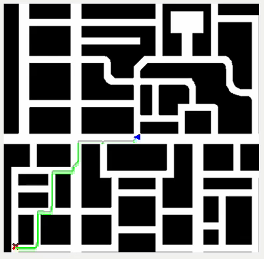
\includegraphics[width=0.4\textwidth]{figures/GPP/Experimento1.png}
		\caption{Imagen del mapa con el primer destino elegido}
		\label{fig.experimento1}
		\end{center}
\end{figure}

\item Segundo destino: En esta ocasión se ha elegido un punto en la plaza, que se podrá ver en la Figura~\ref{fig.experimento2}. Al comprobar el tiempo de planificación se ha obtenido un tiempo de 16’, al igual que en el caso anterior. El tiempo de pilotaje es de 1’ 57’’. En esta ocasión el tiempo de pilotaje ha sido aproximadamente 30’’ más rápido. Si comprobamos el \textit{Real Time} vemos que es de 3’ 06’’; mientras que el \textit{Sim. Time} es de 1’ 35’’. Es decir, en esta ocasión la diferencia entre el tiempo simulado y el tiempo real es menor, lo que nos lleva a obtener un menor tiempo de ejecución.

\begin{figure}[H]
  \begin{center}
    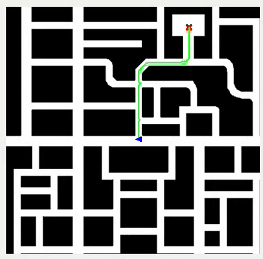
\includegraphics[width=0.4\textwidth]{figures/GPP/Experimento2.png}
		\caption{Imagen del mapa con el segundo destino elegido}
		\label{fig.experimento2}
		\end{center}
\end{figure}

\item Destino a distancia media: El punto escogido lo podemos ver en la Figura~\ref{fig.experimento3}. En este caso el tiempo de la planificación ha sido de 19’, algo superior a las ocasiones anteriores. El tiempo que tarda el taxi en llevar a cabo el pilotaje es de 1’ 12’’, inferior que en el resto de ocasiones puesto que es un destino más cercano. En esta ocasión el \textit{Real Time} ha sido de 2’ 19’’; y el \textit{Sim. Time} ha sido de 1’ 17’’. La diferencia ha sido menor que en las anteriores ocasiones.

\begin{figure}[H]
  \begin{center}
    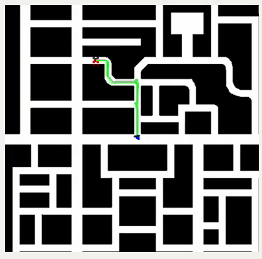
\includegraphics[width=0.4\textwidth]{figures/GPP/Experimento3.png}
		\caption{Imagen del mapa con el segundo destino elegido}
		\label{fig.experimento3}
		\end{center}
\end{figure}
\end{itemize}

Hemos podido comprobar cómo influyen diferentes aspectos en el tiempo de simulación: la lejanía del destino y las capacidades del ordenador que empleemos. Además, hemos observado que el tiempo de planificación suele ser bastante corto, esto es debido a que el algoritmo es rápido. El pilotaje por su parte ha sido más lento debido a distintos aspectos. Sería posible mejorar el tiempo de ejecución empleando quizás algún otro algoritmo más rápido o mejorando el existente. Además, se podría mejorar el tiempo de ejecución dotando al taxi de una mayor velocidad.
\lhead[]{CAPÍTULO \thechapter. ASPIRADORA AUTÓNOMA}
\chapter{Práctica: Aspiradora autónoma}\label{cap.roomba}
En este capítulo se expondrá el desarrollo de una nueva práctica para la plataforma de JdeRobot, que se llamará ``Aspiradora autónoma''. En este capítulo se aborda el desarrollo de la infraestructura, aplicación gráfica, una gráfica de la derivada del porcentaje, así como el evaluador automático creado y la solución llevada a cabo. 

\section{Enunciado de la práctica} \label{sec.enunciado}
El objetivo de esta práctica (llamada aspiradora autónoma) es que una aspiradora robótica sea capaz de limpiar de forma autónoma la mayor cantidad de superficie posible en una casa. La aspiradora no tendrá ninguna forma de obtener su posición en el mundo, ya que el propósito de la práctica es que el algoritmo que se lleve a cabo sea sin autolocalización. El único dato que conocerá la aspiradora es su orientación.  Además, esta aspiradora posee un sensor láser, que le permite medir la distancia a la que se sitúan los obstáculos. Esta aspiradora tiene un actuador de movimiento que se basa en velocidad lineal y velocidad de giro. Todos estos elementos nos deberán permitir realizar un algoritmo de pilotaje para recorrer la casa.\\

En esta práctica el alumno deberá programar el algoritmo capaz de limpiar un gran porcentaje de la casa sin autolocalización. En la interfaz gráfica se puede visualizar un mapa de la casa, así como la posición de la aspiradora en el mapa y los lugares por donde ha pasado. Este mapa no estará disponible para realizar la solución sin autolocalización, el mapa únicamente se utiliza para facilitar el trabajo al alumno.  \\

El algoritmo responde a un control reactivo, que en cada instante actuará en función de los datos de los sensores o del algoritmo que se planifique en cada instante. El control reactivo permitirá controlar en todo momento el entorno que rodea al robot y responder ante situaciones imprevistas.

\section{Infraestructura}
En este apartado se describirá el entorno creado para realizar la práctica ``Aspiradora autónoma''. Además, se describirá el robot que se ha utilizado en esta práctica, así como el entorno por el que se mueve este robot. También se explicarán los sensores y actuadores que tiene el robot.

\subsection{Roomba}
El robot que se ha empleado en esta práctica es el robot Roomba de la serie 500, que fue comercializado por la empresa iRobot (en Estados Unidos). Esta aspiradora robótica está equipada con un conjunto de sensores con los que explorar sus alrededores y unos actuadores que le permiten moverse adecuadamente por su entorno. Los modelos de Roomba de esta serie poseen sensores infrarrojos, un sensor detector de suciedad, un sensor detector de desniveles, y cuentan además con un bumper.\\

En el caso de la práctica, se empleó el modelo de Roomba de JdeRobot, que no tiene detector de desniveles debido a que el escenario de nuestra práctica no contiene desniveles; y tampoco tiene detector de suciedad, puesto que no se ha simulado la suciedad en el mundo de Gazebo ya que el objetivo era realizar el algoritmo de navegación. En nuestro modelo de Roomba tenemos un sensor bumper, que nos permite detectar los choques con objetos; y un sensor láser, que nos permite medir la distancia a los objetos. Este sensor láser es capaz de hacer un barrido de 180 grados, con precisión de 1 grado. Además, este robot posee sensores \acrshort{gps}, los cuales le permiten conocer la posición en la que se encuentra el robot en cada momento.\\

El robot Roomba de la serie 500 posee una anchura de 340 milímetros, 92 milímetros de altura, y un peso de 3.6 kg. El modelo Roomba de JdeRobot mide aproximadamente 330 mm de ancho, 90 mm de altura, y un peso de 2.5 kg.\\

\begin{figure}[H]
  \begin{center}
    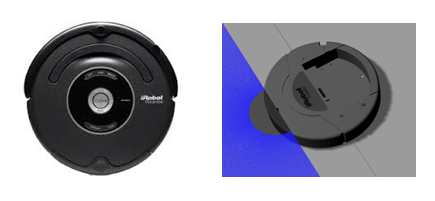
\includegraphics[width=0.6\textwidth]{figures/Vacuum/Roombas.png}
		\caption{Roomba de iRobot y modelo Roomba en Gazebo}
		\label{fig.roombas}
		\end{center}
\end{figure}

\subsection{Sensor láser}
En la parte frontal del robot se ha instalado un sensor láser. Este sensor se utilizará ampliamente en el algoritmo de la práctica. Este sensor láser está compuesto por un array de 180 láseres, esto supone que vamos a tener un láser que puede medir distancia alrededor de 180 grados. Esta cualidad nos permite detectar obstáculos en estos 180 grados, y poder determinar dónde se encuentra aproximadamente. Las medidas de distancia que nos devuelve el láser están en milímetros.\\

Una vez más la plataforma JdeRobot encapsula la complejidad de este sensor y nos devuelve los datos que ofrece el mismo, es decir, los datos de distancia de cada posición del array del láser. 

\subsection{Sensor bumper}
El sensor bumper es un sensor de contacto que nos permite detectar una colisión con un objeto. Esto va a ser muy útil para realizar el algoritmo de esta práctica. Este sensor lo que hace es comprobar el número de contactos con el entorno y si dicho número es mayor que cero es porque el robot ha chocado con algún objeto. La plataforma JdeRobot nos abstrae de realizar el comportamiento complejo de este sensor, y nos permite conocer si ha habido algún choque con algún obstáculo de manera sencilla. La forma que tiene JdeRobot de comunicarnos si hay un choque o no es devolviéndonos un 0 o un 1 en función de si existe choque o no. Si el robot se ha chocado con algún objeto, entonces el bumper nos devolverá un 1. Por el contrario, si el robot no colisiona con ningún obstáculo, entonces el bumper nos dará como resultado un 0.\\

En esta práctica se han utilizado cuatro drivers: 

\begin{itemize}
\item pose3di: Los componentes harán uso de este plugin para obtener su posición en tiempo real. Además, este plugin se emplea para modificar la posición de los componentes.
\item motorsi: Este plugin interactúa con el componente, dotándole de velocidad, tanto velocidad de tracción como velocidad de rotación y modifica los datos de la interfaz de usuario.
\item Laseri: Este plugin será usado por los componentes para poder obtener información de la distancia que hay hasta los obstáculos.
\item Bumperi: El componente podrá usar este plugin para recolectar información acerca de su situación de colisión con otro objeto cualquiera.
\end{itemize}

\subsection{Modelo House}
El propósito de esta práctica es que el robot Roomba sea capaz de recorrer la superficie del suelo de una casa. Por lo tanto, será necesario crear un modelo de casa para poder interactuar en ella. Hemos empleado el modelo de casa que empleo Juan Navarro ~\cite{localization1} en su proyecto en el mundo GrannyAnnie.world (se puede observar en la siguiente imagen), pero hemos realizado algunas modificaciones.\\

\begin{figure}[H]
  \begin{center}
    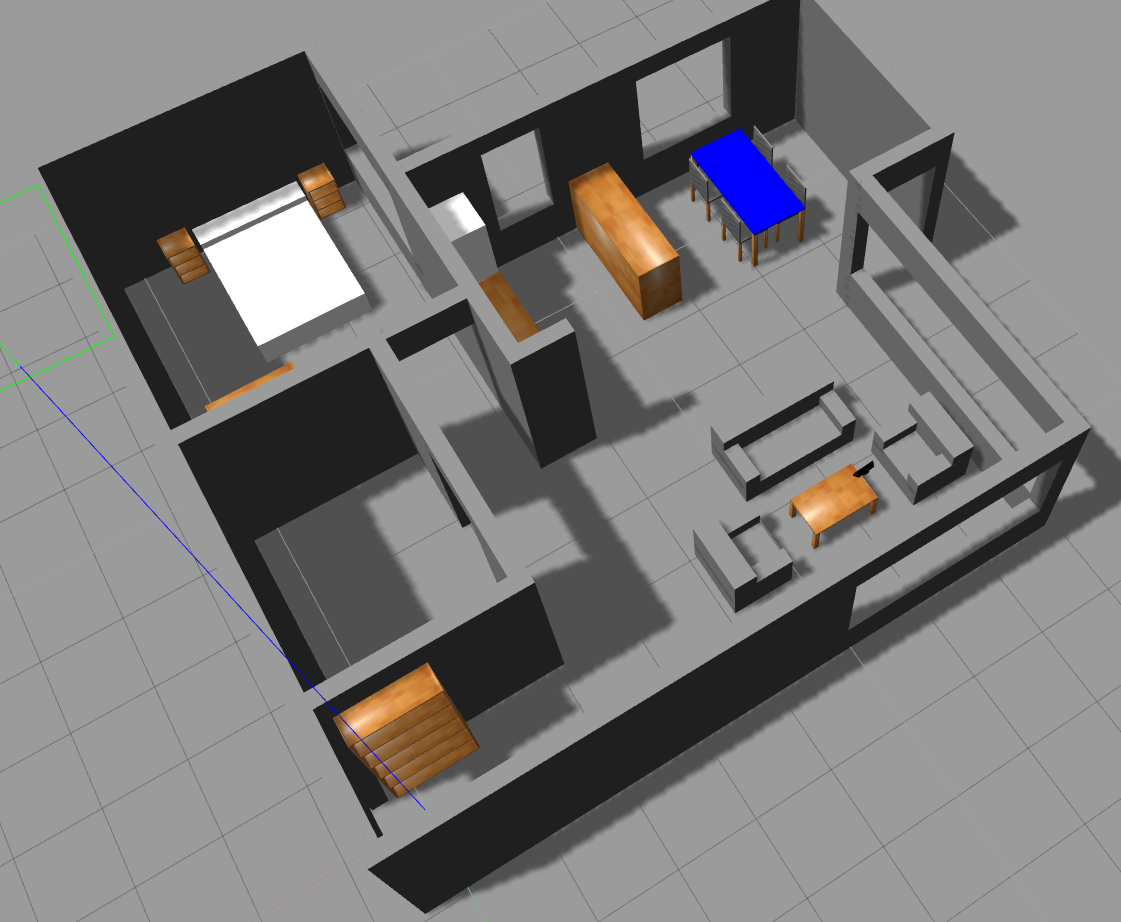
\includegraphics[width=0.6\textwidth]{figures/Vacuum/ModeloCasa_antiguo.png}
		\caption{Mundo GrannyAnnie.world en Gazebo}
		\label{fig.modelocasa_antiguo}
		\end{center}
\end{figure}

Este modelo se ha tenido que modificar puesto que había puertas que daban al exterior de la casa, entonces si pusiéramos a nuestra aspiradora a recorrer la casa se podría salir de la misma y no queremos que suceda esto. Además, se modificó el modelo de la casa debido a que había alguna pared que tenía mal la malla de colisiones, esto hacía que el robot pudiera atravesar algunas paredes. Este era un problema puesto que la casa tiene que ser lo más realista posible, por lo que se modificó la malla de colisiones en algunas zonas de la casa. Además, se modificaron las masas del inmobiliario incrementando su valor. Esto se debe a que la masa que tenían anteriormente no era suficiente y la aspiradora al colisionar con los muebles (mesas, sillones, etc) los desplazaba. El nuevo modelo de casa se llama ``house\_int2'' y lo podemos ver a continuación.\\

\begin{figure}[H]
  \begin{center}
    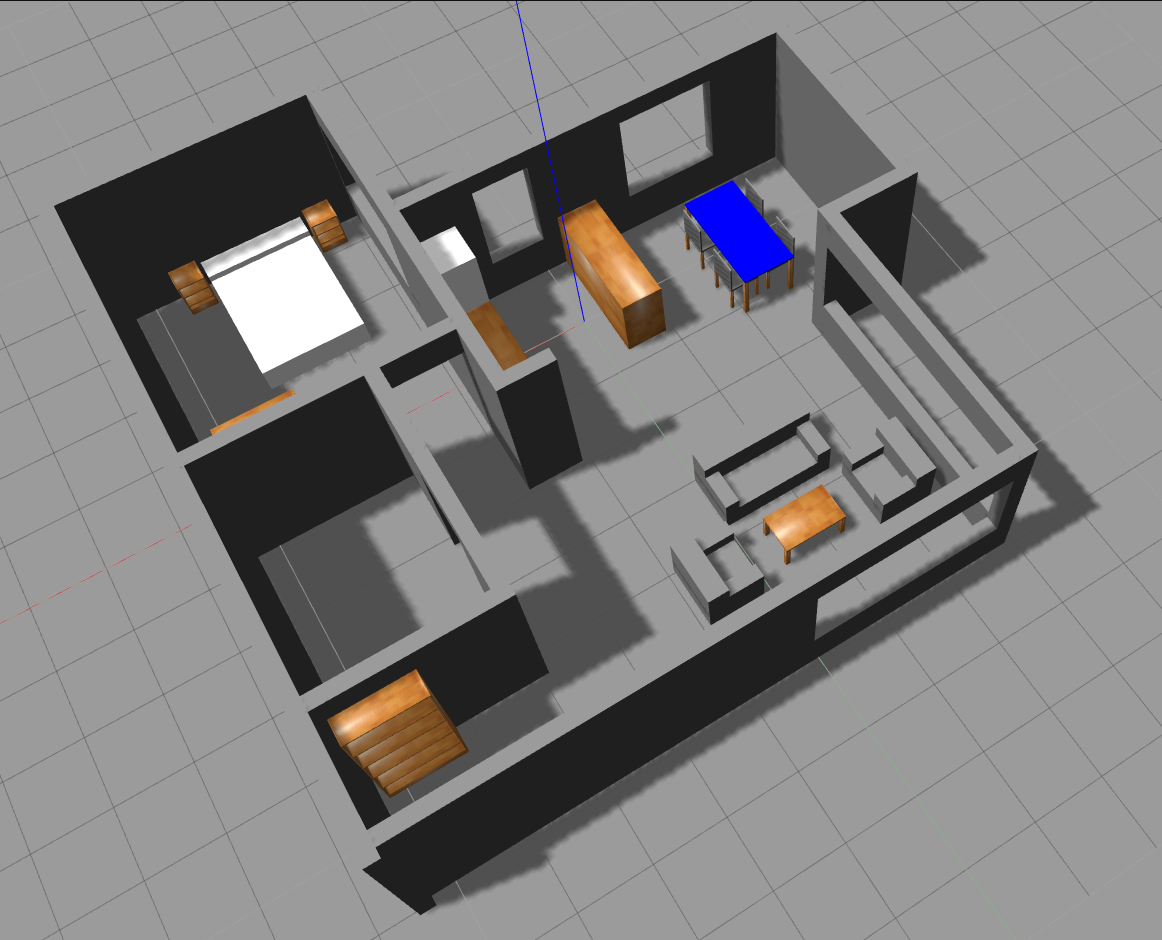
\includegraphics[width=0.6\textwidth]{figures/Vacuum/casa.png}
		\caption{Modelo house\_int2 en Gazebo}
		\label{fig.casa}
		\end{center}
\end{figure}

\subsection{Mundo de Gazebo}
Si queremos ver el comportamiento de la aspiradora dentro de la casa, antes debemos crear un mundo de Gazebo que esté formado por el modelo de la casa ``house\_int2'' y el modelo de aspiradora ``Roomba''. Por este motivo se ha creado un mundo llamado ``Vacuum.world''. Este archivo tiene el siguiente aspecto:

\vspace{20pt}
	\begin{lstlisting}[frame=single]
<?xml version="1.0" ?>
  <sdf version='1.4'>
    <world name=' Vacuum '>
    <include>
      <uri>model://roomba</uri>
        <pose>-1 1.5 0 0 0 0</pose>
    </include>
    <include>
      <uri>model://house_int2</uri>
        <pose>0 0 0 0 0 0</pose>
    </include>
    <include>
      <uri>model://ground_plane</uri>
   </include>

   <light name='sun' type='directional'>
       <cast_shadows>1</cast_shadows>
       <pose>0 0 10 0 -0 0</pose>
       <diffuse>0.8 0.8 0.8 1</diffuse>
       <specular>0.2 0.2 0.2 1</specular>
       <attenuation>
       <range>1000</range>
       <constant>0.9</constant>
       <linear>0.01</linear>
       <quadratic>0.001</quadratic>
       </attenuation>
       <direction>-0.5 0.1 -0.9</direction>
    </light>

    <scene>
        <ambient>0.4 0.4 0.4 1</ambient>
        <background>0.7 0.7 0.7 1</background>
        <shadows>1</shadows>
    </scene>

    <gui fullscreen='0'>
        <camera name='user_camera'>
            <pose>0.126197 6.13852 18.8314 0 1.08764 -2.14299</pose>
            <view_controller>orbit</view_controller>
        </camera>
    </gui>
    </world>
  </sdf>

	\end{lstlisting}

\section{Componente académico}
El componente académico resuelve varias funcionalidades en la práctica: ofrece una interfaz gráfica al usuario, que le ayuda a depurar su código; ofrece acceso a sensores y actuadores en forma de métodos simples (oculta el middleware de comunicaciones); incluye código auxiliar que no es el foco del algoritmo y que ayuda a programar la solución. El componente deja todo preparado para que el estudiante sólo tenga que retocar en MyAlgorithm.py.\\

Este componente ofrece al programador del algoritmo un \acrshort{api} de sensores y actuadores. A continuación, se puede ver el \acrshort{api} concreto de esta práctica:

\begin{itemize}
\item pose3d.getYaw(): Permite obtener la orientación del robot con respecto al mapa.
\item bumper.getBumperData().state: Devuelve un 1 si el robot colisiona y un 0 si no ha chocado.
\item laser.getLaserData(): Permite obtener los datos del sensor láser, que se compone de 180 pares de valores (0-180º, distancia en milímetros).
\item motors.sendV(): Para establecer la velocidad lineal.
\item motors.sendW(): Para establecer la velocidad de giro.

\end{itemize}


Es necesario crear un archivo de configuración (terminado con la extensión .cfg). Este archivo sirve para poder indicar los puertos que utilizan cada uno de los plugins que posee Roomba. Este archivo es necesario para que nuestra aplicación pueda comunicarse con gazeboserver. El archivo de configuración (vacuumCleaner.cfg) en la práctica tiene el siguiente aspecto: 


\vspace{20pt}
	\begin{lstlisting}[frame=single]
VacuumCleaner.Motors.Proxy = Motors:default -h localhost -p 9003
VacuumCleaner.Pose3D.Proxy = Pose3D:default -h localhost -p 9003
VacuumCleaner.Laser.Proxy  = Laser:default -h localhost -p 9003
VacuumCleaner.Bumper.Proxy  = Bumper:default -h localhost -p 9003
VacuumCleaner.Motors.maxV = 5
VacuumCleaner.Motors.maxW = 20

	\end{lstlisting}
	
En el caso de nuestra aspiradora podemos ver que tanto los motores, como la Pose3D, el láser y el bumper emplean el mismo puerto, el 9003. Gracias a cómo está configurado JdeRobot en su versión actual, se puede emplear el mismo puerto. Además, se puede observar que se establece la velocidad de tracción y rotación máxima que tendrán los motores de la aspiradora.\\

La práctica emplea hilos de ejecución para poder realizar diferentes tareas al mismo tiempo, ya que se divide el comportamiento en tareas más sencillas. Esta práctica emplea varios procesos:

\begin{itemize}
\item Hilo de control: Es el encargado de actualizar los datos de los sensores y los actuadores a través de las interfaces \acrshort{gps}. El tiempo de refresco de este hilo es crucial, y tiene que ser un periodo de tiempo muy corto, ya que este componente se encarga de establecer la velocidad y la dirección del robot en todo momento, así como de actualizar los datos de los sensores que son muy importantes para la solución de la práctica. Si este tiempo fuera muy grande, las decisiones que modifican la navegación del robot podrían ser incorrectas. En el caso de esta práctica el hilo de control de actuadores y sensores se actualizará cada vez que se actualiza la \acrshort{gui}, es decir, cada 50 ms.

\item	Hilo de la interfaz gráfica de usuario (\acrshort{gui}): Este hilo es el encargado de actualizar la interfaz gráfica. También consta de los manejadores de eventos del \acrshort{gui}, que son los encargados de ejecutar el código del fichero MyAlgorithm.py. El intervalo de actualización de la interfaz debe ser pequeño, ya que se tiene que mostrar la posición del robot en el mapa que se muestra en la interfaz en tiempo real. Este intervalo de tiempo es de 50 ms.

\end{itemize}


\subsection{Interfaz gráfica de la práctica}
La interfaz gráfica de usuario (\acrshort{gui}) de la práctica sirve para representar información importante que sirve de ayuda para resolver adecuadamente el algoritmo que se plantea. Esta interfaz sirve para poder llevar a cabo diferentes acciones para la ejecución del algoritmo de solución de la práctica. La \acrshort{gui} se programa con PyQt5 y el lenguaje de programación es Python.\\

En la \acrshort{gui} de la práctica se muestra en la esquina superior izquierda el logo de JdeRobot. Este logo es una imagen en RGB, que hemos escalado en la \acrshort{gui} para que se muestre con un tamaño inferior.\\

Esta interfaz contiene una imagen del mapa de la casa por la que navega Roomba. Este mapa es una imagen binaria, donde aparecen con un color negro (valor 0) los obstáculos de la casa, mientras que el suelo, que es la zona por donde podrá navegar la aspiradora, tiene un color blanco (valor 255). Esta imagen es un simple visor de la situación de la aspiradora, ya que este mapa no se proporciona al alumno para la solución de la práctica. En esta imagen del mapa también aparecerá pintada la posición de Roomba como un triángulo (donde solamente se pintan sus aristas) en color rojo. Esto nos permitirá saber dónde está situada nuestra aspiradora en el mapa, así como la orientación que tiene la misma. Pero este triángulo no es el único elemento que se pinta en el mapa de la casa, también se pintará en color azul las zonas de la casa por donde ha pasado la aspiradora en todo momento. Este pintado nos ayudará a ver que la aspiradora hay por zonas por las que puede que haya pasado varias veces, mientras que por otras aún no habrá pasado.\\

Para poder pintar tanto el triángulo como las zonas por donde ha pasado el robot en el mapa, hay que emplear un sistema de conversión del sistema de referencia del mundo (3D) al sistema de referencia del mapa (2D). Para poder pasar del sistema de referencia del mundo al del mapa se han empleado matrices de rotación y traslación, como sucedía en el capítulo anterior. Para poder hacer la conversión de un sistema a otro, lo primero que hay que saber es cómo están situados los sistemas de referencia. En el caso de esta práctica los sistemas de referencia están situados de la siguiente forma:

\begin{figure}[H]
  \begin{center}
    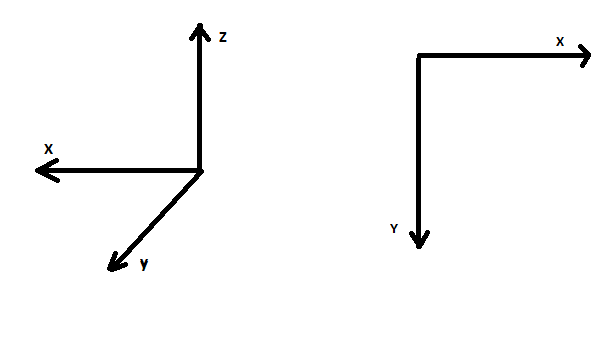
\includegraphics[width=0.6\textwidth]{figures/Vacuum/SistemaRef_world_image.png}
		\caption{Sistema de referencia del mundo (izquierda) y sistema de referencia de la imagen (derecha)}
		\label{fig.sistemaref_world}
		\end{center}
\end{figure}

Para poder saber dónde está situado nuestro robot en la imagen tenemos que pasar de una coordenada (x, y) en 3D a una coordenada (x’, y’) en 2D. Para poder pasar de un sistema en 3D a un sistema 2D se ha aplicado una matriz de rotación y traslación. En concreto, se aplica una rotación de pi grados (será el ángulo \(\alpha\) de la matriz) sobre el eje y. La traslación se realiza porque queremos tener el punto (0,0) de la imagen en la esquina superior izquierda, y para que se corresponda correctamente cada punto de la imagen con cada punto del mundo. En este caso la traslación que se ha aplicado es de 0.6 (será tx) en el eje x; y -1 (será ty) en el eje y. La matriz de rotación y traslación sobre el eje y es la siguiente:


\begin{equation}
\left[\begin{array}{cc}
x' \\ 
y' \\
z' \\
1
\end{array}\right] = \left[\begin{array}{cccc}
\cos(\alpha) & 0 & \sin(\alpha) & tx \\ 
0 & 1 & 0 & ty\\
-\sin(\alpha) & 0 & \cos(\alpha) & tz \\
0 & 0 & 0 & 1
\end{array}\right]* \left[\begin{array}{cc}
x \\ 
y \\
z \\
1
\end{array}\right]
\end{equation}
\\

De esta forma podemos pintar el triángulo que es la representación de la aspiradora en la casa, pasando la coordenada del mundo que nos devuelve el pose3d a coordenada en la imagen, la cual será el centro del triángulo que dibujaremos con una pequeña desviación. El triángulo es un triángulo isósceles para poder distinguir cuál es la orientación del robot. La aspiradora estará orientada hacia el vértice que posee un ángulo menor que el resto.\\

Esta rotación también nos sirve para poder pintar en azul los puntos del mapa por donde ha pasado la aspiradora en cualquier momento. Se pintará un círculo en cada iteración dado que la aspiradora ocupa un determinado volumen. Los puntos por los que ha pasado la aspiradora se guardan en un array para poder saber por dónde ha pasado y pintarlos todos en cada iteración.\\

Por otra parte, en la esquina superior derecha de la \acrshort{gui}, tenemos un teleoperador para teleoperar el robot. Este teleoperador controla las velocidades lineal y angular del robot. La velocidad lineal del robot se puede controlar moviendo el joystick en sentido vertical. Cuanto más subamos el joystick más velocidad tendrá el robot hacia delante, y si lo bajamos del todo más velocidad lineal tendrá el robot hacia atrás. La velocidad angular del robot se controla moviendo el joystick en sentido horizontal, según lo movamos a izquierda o a la derecha, el robot girará en un sentido u otro.\\

En la aplicación gráfica hay dos botones, que son bastante importantes para la práctica. El botón superior que aparece con un símbolo de stop es el botón que emplearemos cuando teledirigimos a la aspiradora y queremos que pare en un punto y no siga navegando. El botón inferior, en el cual pone ``Run my algorithm'', es el botón con el que le ordenaremos a la práctica que comience a ejecutar la solución que se ha programado en el fichero MyAlgorithm.py. Si queremos que este código pare en un determinado momento, pulsaremos el mismo botón haciendo que pare; y si queremos reanudar su comportamiento lo volveremos a pulsar.\\

Podemos ver cómo es esta interfaz en la Figura~\ref{fig.GUI2}:

\begin{figure}[H]
  \begin{center}
    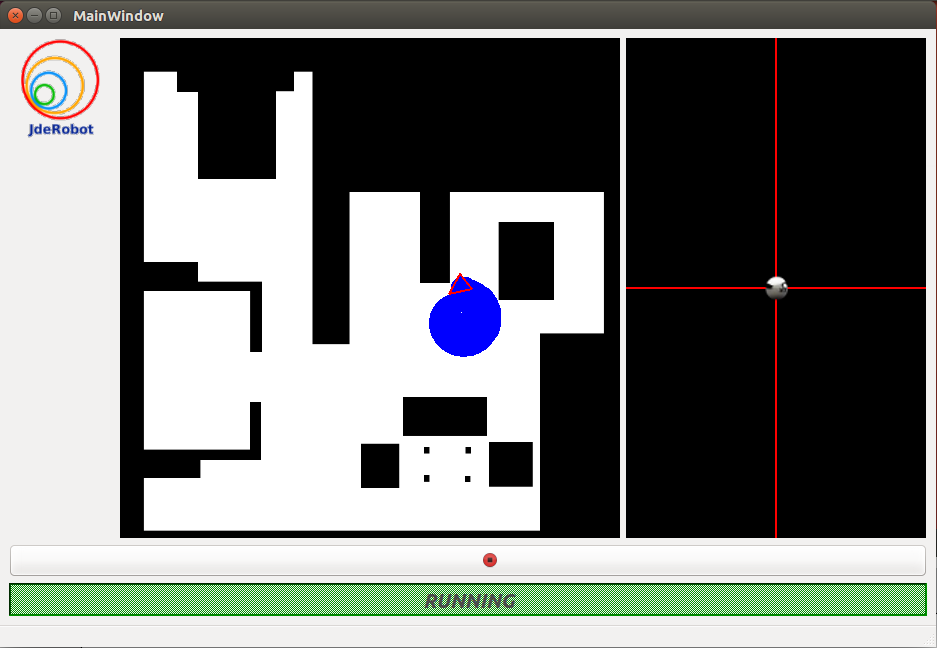
\includegraphics[width=0.7\textwidth]{figures/Vacuum/GUI2.png}
		\caption{Interfaz gráfica (\acrshort{gui}) de Vacuum después de un tiempo de ejecución}
		\label{fig.GUI2}
		\end{center}
\end{figure}

\subsection{Gráfica de la derivada del porcentaje}
En esta práctica se ha decidido crear una gráfica de la derivada del porcentaje en función del tiempo para poder comprobar cómo evoluciona el porcentaje de casa recorrido durante el tiempo.\\

La derivada de y (se representa en el eje vertical) respecto a x (se representa en el eje horizontal) es lo que varía y por cada unidad que varía x. Se puede designar este valor como dy/dx. Las expresiones dy y dx se llaman, respectivamente, diferencial de y, y diferencial de x. dx es la variable independiente y dy la variable dependiente de la función diferencial. Es decir, podemos ver que la derivada representa la diferencia de y respecto la diferencia de x. \\

En el caso de nuestra práctica, siguiendo esta definición de la derivada, podemos definir la derivada del porcentaje (eje vertical) respecto del tiempo (eje horizontal) como la diferencia del porcentaje cada unidad de diferencia del tiempo.\\

En la práctica en el eje vertical se representa la diferencia del porcentaje cada cierto tiempo. En el eje horizontal se representan las diferencias de tiempo, que siempre representan el mismo intervalo de tiempo. \\

En este caso, en el eje horizontal se representa el tiempo, el cual se divide en 9 intervalos de tiempo. Cada intervalo de tiempo que se representa, en el eje horizontal, se corresponde con un intervalo de 100 segundos. Por lo tanto, en la práctica vamos a observar el comportamiento del porcentaje a lo largo de 900 segundos, es decir, 15 minutos.\\

En el eje vertical, se representa la diferencia de porcentaje en cada intervalo de tiempo. Es decir, por ejemplo, en el primer intervalo de tiempo se representará la diferencia de porcentaje recorrido entre el segundo 100 de la práctica y el segundo 0. Así, sucederá para cada uno de los intervalos.\\

De esta forma, esta gráfica nos permitirá ver cómo evoluciona el porcentaje recorrido respecto al tiempo. Cuando la aspiradora realiza el algoritmo de navegación puede que en ciertas ocasiones pase varias veces por una misma zona o se quede un rato atascada en ciertas zonas. Es decir, que al principio cuando ejecutamos la práctica es muy sencillo que nuestra aspiradora recorra un gran porcentaje de casa, pero más adelante será más complicado que pase por zonas por las que no había pasado. Esto implica que posiblemente la derivada del porcentaje en función del tiempo sea mayor al comienzo de la ejecución de la práctica que por el final. Cada vez que se ejecute la práctica esta gráfica variará.\\

Esta gráfica tendrá 9 escalones en el eje horizontal como hemos mencionado antes, y 5 escalones (cada uno representa una diferencia del 2\%) en el eje vertical. La gráfica se representa en color rojo.En la Figura~\ref{fig.grafica_percentaje2} se puede observar un ejemplo de la gráfica de la derivada del porcentaje recorrido en función del tiempo.\\

\begin{figure}[H]
  \begin{center}
    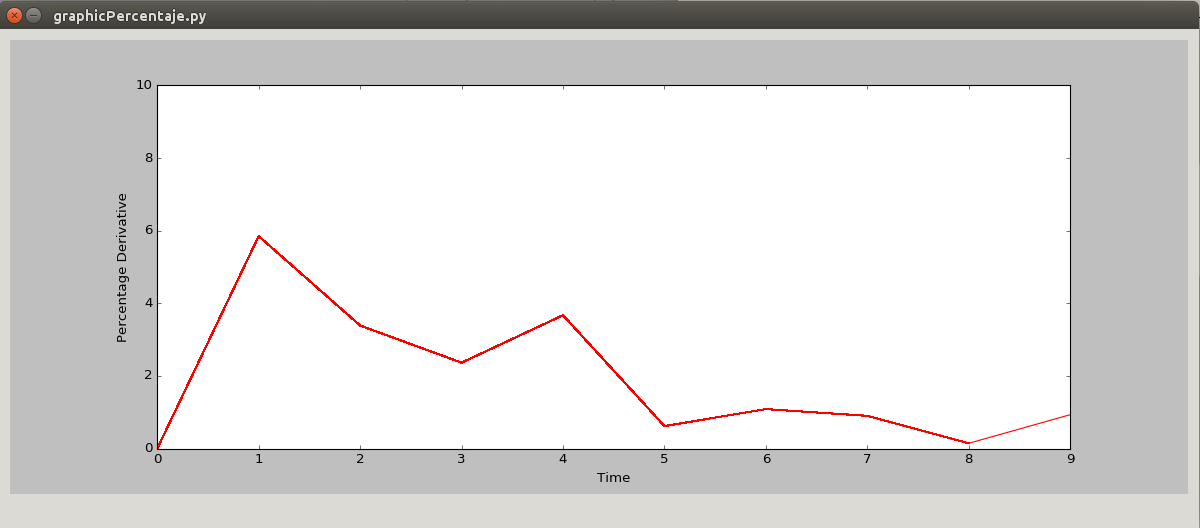
\includegraphics[width=0.9\textwidth]{figures/Vacuum/Grafica_percentaje2.png}
		\caption{Gráfica de la derivada del porcentaje en función del tiempo}
		\label{fig.grafica_percentaje2}
		\end{center}
\end{figure}

\section{Solución de referencia}
Como hemos observado en el Apartado~\ref{sec.enunciado}, el objetivo de esta práctica es proveer al robot de un algoritmo de navegación, que responde a un control reactivo. En este punto abordaremos una breve explicación sobre algoritmos que emplean aspiradoras robóticas disponibles en el mercado, una descripción de la técnica que emplea Roomba de iRobot, y la solución concreta de la práctica. El fichero MyAlgorithm.py es de naturaleza iterativa, ejecuta continuamente iteraciones y en cada una de ellas se percibe y se controla.


\subsection{Algoritmo empleado por distintas aspiradoras robóticas}
En los últimos 15 años, han aparecido múltiples modelos de aspiradoras robóticas, las cuales son cada vez más innovadoras. Es importante tener en cuenta los algoritmos de navegación que llevan a cabo cada uno de los modelos, ya que en función de estos algoritmos la aspiradora limpiará en menor o mayor tiempo la casa. Además, es importante tener en cuenta en estos algoritmos los posibles obstáculos con los que se encontrará la aspiradora al recorrer la casa. A continuación, podemos ver diferentes algoritmos de navegación que existen hoy en día en función del modelo:

\begin{itemize}
\item Uno de los primeros modelos de aspiradora Trilobite de Electrolux navega empleando ultrasonidos. Esta aspiradora usa la siguiente estrategia de navegación: explora el perímetro del entorno (siguiendo un comportamiento de sigue la pared); después de que la aspiradora llegue al punto de partida donde comenzó a recorrer la pared, el robot estima el tamaño del entorno y comienza con una trayectoria aleatoria.
\begin{figure}[H]
  \begin{center}
    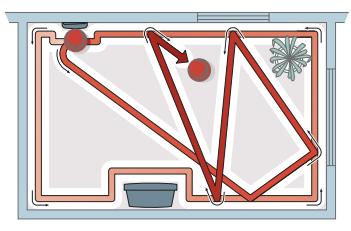
\includegraphics[width=0.6\textwidth]{figures/Vacuum/Trilobite.png}
		\caption{Patrón de navegación de la aspiradora Trilobite}
		\label{fig.Trilobite}
		\end{center}
\end{figure}
\item El sistema de navegación de la aspiradora robótica Xiaomi está guiado por un láser. Utiliza el algoritmo \acrfull{slam} para generar un mapa de la casa en la que se encuentra y calcula patrones inteligentes para moverse a través de la casa. Xiaomi afirma que su modelo de aspiradora no solamente sigue un mapa y trata de limpiar el 100\% de la superficie del suelo de la casa, simplemente siguiendo las instrucciones, sino que en realidad su aspiradora puede pensar y calcular el mejor patrón de limpieza para la casa.  Cuando arranca Xiaomi, hace un escaneo de la zona circundante y divide la habitación en secciones de aproximadamente 4 por 4 metros. A continuación, el robot realiza un barrido del perímetro alrededor de esta área seccionada, trazando los obstáculos que puedan interponerse en el camino de la trayectoria. Después, ``rellena'' esta sección haciendo barridos horizontales.
\begin{figure}[H]
  \begin{center}
    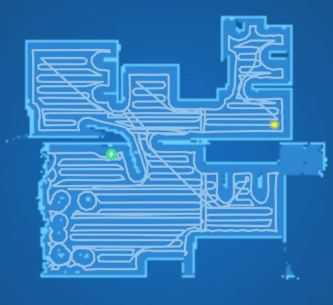
\includegraphics[width=0.4\textwidth]{figures/Vacuum/Xiaomi.png}
		\caption{Patrón de navegación de la aspiradora Xiaomi}
		\label{fig.Xiaomi}
		\end{center}
\end{figure}
\item También es importante destacar la gama de robot LG Hombot. Vamos a analizar en concreto el sistema de navegación del LG Hombot Turbo. Este aspirador es capaz de crear un mapa de la superficie, memorizando cada obstáculo, evitando el movimiento aleatorio y minimizando los choques. 
\item El más conocido de las aspiradoras robóticas es Roomba de iRobot. Roomba posee diferentes modelos, desde los más antiguos hasta los más innovadores. Existen grandes diferencias entre estos en cuanto a su patrón de limpieza. Los modelos de las series 500, 600, 700 y 800, calculan la ruta de limpieza óptima y determinan cuándo es necesario utilizar sus diversos modos de limpieza: giro en espiral, seguimiento de paredes, cruce de habitación. En cambio, los modelos de la serie 900 de Roomba, tienen navegación iAdapt 2.0, se adaptan al entorno y disponen de localización visual para limpiar. A través de la localización visual, crea un mapa con referencias, para recorrer toda la casa y saber por dónde ha pasado y dónde tiene que ir. Limpia de forma eficiente en áreas abiertas moviéndose en líneas paralelas mientras que, gracias a los sensores, adapta su trayectoria cuando se necesita limpiando de forma eficiente.
\end{itemize}

Estos modelos que acabamos de mencionar son solamente unos pocos dentro de una amplia variedad de modelos de aspiradoras robóticas que existen hoy en día.\\

Es importante destacar que todos los modelos de aspiradora usan diferentes modos de limpieza (espiral, zig-zag, aleatorio, recorrer bordes, etc) en función de la zona de la casa donde se encuentren o en función de qué es lo que más le interesa a su dueño.\\

Con la descripción de los patrones que emplean las aspiradoras anteriores, podemos deducir que existen modelos de aspiradoras que emplean patrones aleatorios para poder limpiar la casa; y, por otro lado, hay otros modelos que inicialmente se construyen un mapa de la casa para recorrer la superficie de una forma más óptima.

\subsection{Algoritmo empleado por Roomba serie 500, 600, 700, 800}
Para resolver el algoritmo sin autolocalización que se plantea en la práctica nos hemos basado en el algoritmo de navegación que siguen los modelos de las series 500, 600, 700 y 800 de Roomba, que no emplean un mapa de la casa para poder realizar el algoritmo. A continuación, se explicará cómo navega Roomba por su entorno.\\

Mientras Roomba está limpiando evita caerse por las escaleras o por un terreno empinado. Esto lo hace gracias a cuatro sensores infrarrojos en la parte inferior delantera. Estos sensores envían constantemente señales de infrarrojos, y si estas señales se pierden es porque el robot ha llegado a una zona de elevada pendiente por donde podría caerse. De esta forma es como Roomba evita caerse por pendientes al dirigirse hacia otra zona.\\

Cuando Roomba choca con un objeto el bumper se retrae, activando sensores de objetos mecánicos que le avisan a Roomba de que ha chocado. Cuando se produce este hecho la aspiradora gira y avanza hasta que encuentra una ruta clara.\\

Esta aspiradora tiene otro sensor de infrarrojos (llamado Wall sensor) situado en la parte delantera del robot. Este sensor permite que Roomba navegue muy de cerca de las paredes, los objetos, etc. \\

Cuando presionamos el botón ``Clean'', lo primero que hace Roomba es calcular el tamaño de la habitación según la información que recibe a través de sus sensores. Este robot envía una señal infrarroja y comprueba el tiempo que tarda en volver la señal. De esta manera calcula el tiempo que tendrá que pasar limpiando. Esto le permite a Roomba optimizar la cobertura por habitación. El tiempo de funcionamiento depende del tamaño de la habitación y de la carga de la batería. Por lo que el robot sabe el tiempo que debe estar limpiando la habitación.\\

Roomba calcula su algoritmo 67 veces por segundo, obteniendo constantemente la información sobre su entorno y recomponiendo su trayectoria.\\

Roomba comienza a limpiar siguiendo un patrón de espiral. Esta espiral se va haciendo cada vez más grande, saliendo la espiral hacia fuera sobre un área más grande y más grande hasta que golpee un objeto. Cuando Roomba encuentre un objeto, seguirá a lo largo de este objeto recorriendo el perímetro de la habitación durante un periodo de tiempo determinado. Cuando pase este periodo de tiempo, Roomba comenzará el modo cruce de la habitación, tratando de averiguar la máxima distancia que puede navegar sin chocar con un objeto. Sin embargo, si lleva un periodo de tiempo grande navegando sin chocarse con ningún obstáculo va a comenzar otra vez a realizar la espiral, porque supone que está en un amplio espacio abierto.\\

Los patrones que eligieron los creadores de Roomba se basan en los algoritmos basados en los comportamientos de los animales cuando van buscando áreas de comida.\\

Este algoritmo de navegación es bastante eficaz y robusto en situaciones del mundo real. A continuación, podemos observar en las imágenes el patrón de comportamiento que sigue la aspiradora Roomba.\\

\begin{figure}[H]
  \begin{center}
    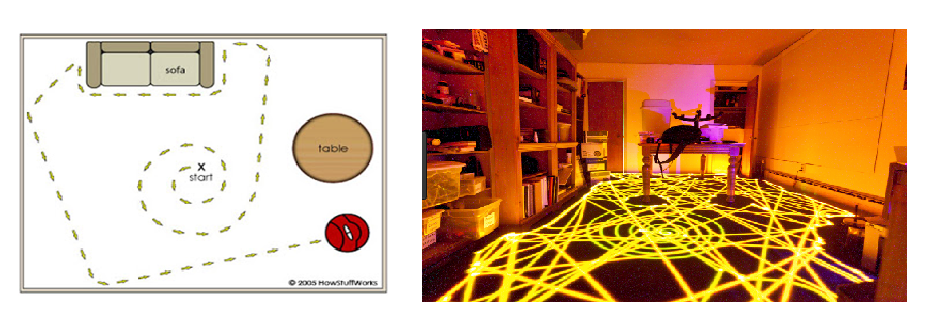
\includegraphics[width=1\textwidth]{figures/Vacuum/Algoritmo_roomba.png}
		\caption{Algoritmo de navegación de Roomba}
		\label{fig.Algoritmo_roomba}
		\end{center}
\end{figure}

\subsection{Solución desarrollada}
Las aspiradoras de hoy en día limpian de diversas formas, unas utilizan autolocalización, mientras que otras no. En el caso de esta práctica, el algoritmo de solución debe ser sin autolocalización, por lo que la aspiradora no conocerá el mapa de la casa, ni sabrá dónde está situada. Existen, también, muchos algoritmos donde las aspiradoras no tienen localización. Sin embargo, hemos optado por basarnos en el algoritmo que realizan los modelos 50, 600, 700 o 800 de Roomba de iRobot. La solución implementada se describirá a continuación. \\

La solución se desarrolla en el fichero ``MyAlgorithm.py''. En este fichero, la solución se desarrollará en el método ``execute'', el cual se ejecuta periódicamente. De esta forma, el pilotaje se llevará a cabo como un control reactivo, es decir, la aspiradora podrá comprobar los datos de sus sensores en cada instante y basándose en estos datos optar por realizar una acción u otra. En el caso de esta práctica, podemos ver que no se realiza ningún tipo de planificación, sino que se lleva a cabo el pilotaje directamente.\\

El primer paso que lleva a cabo Roomba, en la práctica, es realizar una navegación siguiendo un patrón en espiral (al igual que lo hacía la Roomba real). Si queremos realizar un patrón en espiral debemos elegir qué tipo de espiral queremos que intente realizar nuestra aspiradora, ya que existen numerosos tipos de espiral. Algunos de los tipos de espiral son: espiral de Arquímedes, espiral logarítmica, espiral hiperbólica, espiral de Fermat, espiral de Durero, etc. En el caso de esta práctica se ha optado por realizar la espiral de Arquímedes, que es uniforme. Esta espiral se define como el lugar geométrico de un punto moviéndose a velocidad constante sobre una recta que gira sobre un punto de origen fijo a velocidad angular constante. En la siguiente imagen se puede ver el patrón que sigue la espiral de Arquímedes.\\

\begin{figure}[H]
  \begin{center}
    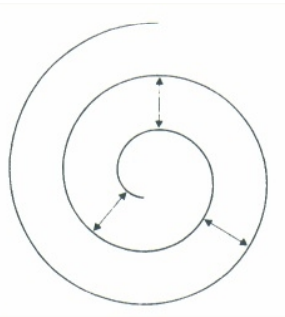
\includegraphics[width=0.3\textwidth]{figures/Vacuum/Espiral_Arquimedes.png}
		\caption{Espiral de Arquímedes}
		\label{fig.Espiral_Arquimedes}
		\end{center}
\end{figure}

Para que la aspiradora pueda realizar un patrón de este tipo, debe tener una velocidad angular constante y una velocidad lineal incremental. Es decir, la velocidad lineal irá aumentando en cada iteración un determinado valor. En el caso de esta práctica se ha optado por tomar como velocidad lineal la multiplicación de dos valores (los cuales inicialmente son valores muy pequeños). Un valor de radio inicial será multiplicado por una variable, la cual irá aumentando en cada iteración. El valor del radio inicial es de 0.1, mientras que la variable inicialmente posee un valor de 0.01. Esta variable será incrementada un 0.012 en cada iteración. De esta forma obtenemos un patrón en espiral similar a la espiral de Arquímedes.\\

Esta espiral se va haciendo cada vez más grande, saliendo la espiral hacia fuera sobre un área más grande. Roomba seguirá este patrón en espiral hasta que choque con un obstáculo. A continuación, podemos ver el patrón en espiral que ha realizado la aspiradora al ejecutar la práctica.\\

\begin{figure}[H]
  \begin{center}
    \includegraphics[width=0.5\textwidth]{figures/Vacuum/Espiral_Roomba.png}
		\caption{Espiral que realiza Roomba en la práctica}
		\label{fig.Espiral_Roomba}
		\end{center}
\end{figure}

Cuando Roomba choca con un obstáculo, sigue a lo largo de este obstáculo recorriendo el perímetro de la casa durante un determinado periodo de tiempo. En el caso de esta práctica, el periodo de tiempo que Roomba realiza el patrón del perímetro es de 300 segundos. Se ha optado por esta duración porque en las pruebas que se han realizado es el que mejores resultados presentaba.\\

Para poder seguir el perímetro se han empleado los datos que recoge el sensor láser que posee Roomba. Para poder obtener los datos del sensor láser se tiene que emplear la función laser.getLaserData(). Esta función nos devuelve 180 pares de valores, que se componen del ángulo y la distancia.\\

Lo primero que hace Roomba es separarse un poco de la pared para no rozar todo el rato con ella. Después gira un poco hasta que encuentra que tiene la pared a su derecha. Para saber si tiene la pared a la derecha emplea el valor de distancia del ángulo 0 (rayo del láser que está a la derecha de Roomba) y el ángulo 45 del array de 180 pares de valores, que mencionamos antes. Para obtener la distancia de cada ángulo se emplea la función distanceData[ángulo]. Un punto importante a tener en cuenta es que la distancia que devuelve el láser es en milímetros.  \\

Tras saber que ya tenemos la pared a la derecha de la aspiradora, podemos recorrer el perímetro. Para ello hay que comprobar continuamente el láser frontal (situado en el ángulo 90). Este láser se comprueba para saber si la aspiradora está en una esquina, ya que en este caso la distancia que obtiene el láser será muy pequeña. Si se da el caso de que se encuentra en una esquina, Roomba girará a la izquierda 90 grados. \\

Otro dato que comprobará es si el láser del ángulo 135 (más a la izquierda) tiene una distancia muy pequeña y además ha detectado un choque. Esto supone que nuestra aspiradora se ha quedado enganchada en algún hueco. Si se da este caso la aspiradora retrocede un poco y gira hacia la izquierda 90 grados.\\

Si la aspiradora no se encuentra en una esquina y no se ha quedado atascada en algún hueco, entonces la aspiradora recorrerá el perímetro siguiendo la pared. Para ello, se comprueba el láser derecho (ángulo 0) y el láser del ángulo 45. Este algoritmo se realiza de forma reactiva comprobando continuamente los datos y tomando decisiones en base a ellos. Si la distancia a la pared es demasiado pequeña es que estamos muy pegados a la pared. En este caso la aspiradora gira un poco a la izquierda para no chocarse con la pared. Si el valor de distancia, por el contrario, es muy grande, entonces gira un poco a la derecha para no desviarse de la pared. Si la distancia a la pared no es ni muy pequeña, ni muy grande, es que podemos seguir adecuadamente la pared tomando una velocidad lineal constante y una velocidad angular nula.\\

Teniendo en cuenta todas estas situaciones que se pueden dar al recorrer la pared, la aspiradora recorre el perímetro correctamente. En la siguiente imagen se puede ver cómo después de realizar el patrón en espiral, Roomba ha realizado el perímetro durante un intervalo de tiempo.\\

\begin{figure}[H]
  \begin{center}
    \includegraphics[width=0.5\textwidth]{figures/Vacuum/Perimetro_Roomba.png}
		\caption{Perímetro que recorre Roomba en la práctica}
		\label{fig.Perimetro_Roomba}
		\end{center}
\end{figure}

El siguiente paso que se lleva a cabo es un algoritmo aleatorio, que realiza un cruce de habitación (similar a la Roomba real). Lo que hace en este caso Roomba es comprobar si la aspiradora ha chocado o no continuamente, es decir, se comprueba si choca en cada iteración. Si ha chocado entonces la aspiradora retrocede un poco para apartarse de la pared, y calcula un ángulo aleatorio y el signo aleatoriamente. Este ángulo que se calcula aleatoriamente es el ángulo que girará Roomba para tomar una nueva orientación El signo que calculamos aleatoriamente es para que nuestra aspiradora gire algunas veces hacia la izquierda y otras veces a la derecha, dotando al algoritmo de mayor aleatoriedad. Para elegir el signo se emplea una función que proporciona Python para calcular aleatoriamente números enteros. En este caso se define un número entre 0 y 1. Si el signo sale 0, entonces Roomba gira a la derecha; si por el contrario es 1, gira a la izquierda.\\

Tras calcular el ángulo y el signo aleatoriamente, Roomba gira hasta haber girado el ángulo que se le ha indicado. Cuando ha realizado el giro, la aspiradora toma como velocidad de giro 0 y toma una velocidad lineal constante. De esta forma Roomba irá recta hacia la orientación que se haya quedado después del giro. Roomba seguirá la recta hasta que vuelva a chocar. Cuando choque volverá a realizar el algoritmo aleatorio hasta finalizar el tiempo de la práctica.\\

A continuación, se muestra la imagen del evaluador automático al finalizar el periodo de tiempo de la práctica. Se puede ver que se ha recorrido el 28 \% de la casa y que se ha obtenido en este caso una nota de 9.33. Tras esta imagen, tenemos otra imagen de la gráfica que representa la derivada en función del tiempo al finalizar la práctica.\\


\begin{figure}[H]
  \begin{center}
    \includegraphics[width=0.6\textwidth]{figures/Vacuum/Referee_Roomba.png}
		\caption{Evaluador automático con la nota final}
		\label{fig.Referee_Roomba}
		\end{center}
\end{figure}

\begin{figure}[H]
  \begin{center}
    \includegraphics[width=0.9\textwidth]{figures/Vacuum/Porcentaje_Roomba.png}
		\caption{Gráfica de la derivada del porcentaje según en tiempo al finalizar la práctica}
		\label{fig.Porcentaje_Roomba}
		\end{center}
\end{figure}

En esta gráfica podemos ver cómo la derivada del porcentaje es mayor al comienzo de la práctica que en el resto de tiempo. Aunque se puede ver que hay algunos picos, donde baja su valor y luego aumenta.


\section{Evaluador automático}
En esta práctica se ha creado un evaluador automático, que en función de diferentes parámetros califica el algoritmo que programa el alumno como solución. El evaluador automático muestra en una interfaz gráfica diferentes parámetros, así como la nota que obtiene el alumno. Este evaluador automático se ha creado utilizando PyQt5 al igual que la aplicación gráfica. Para programar el evaluador automático se han creado clases diferentes para cada parámetro que queramos mostrar en la interfaz. Estas clases serán instanciadas en una clase principal (llamada MainWindow), que será la clase que contiene la ventana principal de la aplicación del evaluador automático.\\

En la esquina superior izquierda, la aplicación del evaluador automático tiene un visor que muestra una barra de progreso. En esta barra se pinta en rojo el porcentaje de superficie recorrida por la aspiradora en cada momento. Encima de esta barra se mostrará un mensaje con el tanto por ciento de superficie recorrida. El porcentaje de superficie recorrida se calcula teniendo en cuenta que el 100\% de superficie que puede recorrer la aspiradora es el suelo donde no hay obstáculos situados. Es decir, el 100\% de superficie que se puede recorrer son todos los píxeles en blanco que aparecen en el mapa que muestra la interfaz.\\

En la esquina inferior izquierda de la aplicación se muestra la imagen del mapa de la casa. Esta imagen es una imagen binaria, en la cual los píxeles blancos (valor 255) representan la zona libre de obstáculos por donde puede navegar la aspiradora (el suelo). Los píxeles en negro (valor 0) representan a los obstáculos que hay en la casa. En esta imagen también se pinta en azul las zonas por donde ha pasado la aspiradora en cualquier momento. Para ello se guardan las posiciones por las que pasa en un array, y se pinta en cada iteración.\\

En la esquina superior derecha de la aplicación, tenemos un visor que muestra un reloj digital. En este reloj se muestran segundos, pero estos segundos no van aumentando según va pasando el tiempo. Por el contrario, los segundos van disminuyendo, es decir, se muestra una cuenta atrás de segundos. Este visor comienza mostrando 900 segundos (que son 15 minutos) y cada vez que ha pasado un segundo lo va descontando de este valor. Se muestran 15 minutos porque se ha considerado un intervalo de tiempo adecuado para evaluar la práctica, ya que si pusiéramos un intervalo mayor de tiempo sería un tiempo excesivo para evaluar la práctica. Sin embargo, si ponemos un intervalo de tiempo menor a 15 minutos no se podría evaluar la práctica con claridad, ya que en los primeros minutos de la práctica es muy sencillo recorrer bastante porcentaje de suelo comparando con los minutos posteriores.\\

Debajo de este visor del tiempo digital se muestra un visor de un reloj analógico. En este reloj analógico sí que avanza el tiempo, al contrario que sucedía con el reloj digital. Este tiene pintadas 60 ``rayitas'' que se corresponden con 60 segundos. En este reloj aparecen pintadas dos manecillas, la más alargada se corresponde con la manecilla de los segundos, y la más corta con la manecilla de los minutos. Conforme haya pasado un segundo la manecilla de los segundos apuntará al siguiente segundo. Lo mismo sucederá con la manecilla de los minutos.\\

En la esquina inferior derecha, se representa una imagen del logo de JdeRobot. Esta imagen es una imagen RGB y ha sido escalada a un tamaño menor.\\

Por último, hay que mencionar que cuando terminen los 900 segundos, a la derecha del reloj digital aparecerá un mensaje con la nota que ha obtenido el alumno. Esta nota se calculará en función del porcentaje recorrido por la aspiradora al pasar 900 segundos. Se ha establecido un porcentaje máximo para estos 15 minutos, ya que no es posible recorrer toda la casa en este tiempo. Este porcentaje es de 30\%. Si la aspiradora recorre un 30\% o más, el alumno obtendrá una nota de 10 puntos. Si por el contrario, la aspiradora recorre menos porcentaje, entonces se calcula la nota haciendo una regla de tres sabiendo que una nota de 10 es un 30\%.\\

En las Figura~\ref{fig.Referee_Vacuum2}, podremos ver el evaluador automático durante el pilotaje.

\begin{figure}[H]
  \begin{center}
    \includegraphics[width=0.6\textwidth]{figures/Vacuum/Referee_Vacuum2.png}
		\caption{Evaluador automático durante la ejecución de la práctica}
		\label{fig.Referee_Vacuum2}
		\end{center}
\end{figure}


\section{Experimentación}
La práctica se ejecuta abriendo cuatro terminales y escribiendo lo siguiente en cada uno de ellos:

\begin{itemize}
\item Lanzar Gazebo: gazebo Vacuum.world
\item	Ejecutar la práctica y lanzar la interfaz gráfica (\acrshort{gui}): python2 vacuumCleaner.py -- --Ice.Config=vacuumCleaner.cfg
\item	Ejecutar la gráfica de la derivada del porcentaje: python2 graphicPercentaje.py -- --Ice.Config=vacuumCleaner.cfg
\item	Ejecutar el evaluador automático: python2 referee.py -- --Ice.Config=vacuumCleaner.cfg

\end{itemize}

Si el ordenador que se emplea no tiene muchos recursos se puede arrancar el simulador sin interfaz gráfico:

\begin{itemize}
\item Lanzar Gazebo: gzserver Vacuum.world
\end{itemize}

En la práctica se decide evaluar 15 minutos, ya que un tiempo mayor supone demasiado tiempo para evaluar una práctica. Por el contrario, si fuera menor el tiempo, es muy probable que se obtuvieran resultados similares, ya que al comienzo de la práctica es más sencillo que aumente el porcentaje de suelo recorrido. Al ser un algoritmo en parte aleatorio, es probable que la aspiradora pase por un mismo sitio varias veces, por lo que no aumentará el porcentaje de superficie recorrida.\\

Un punto importante de la práctica es decidir cuál es el periodo de tiempo que la aspiradora recorrerá el perímetro. En la práctica se ha optado por recorrer el perímetro durante 300 segundos. Para poder elegir un periodo de tiempo se han hecho pruebas con diferentes periodos de tiempo en el que Roomba recorría el perímetro. Se han realizado tres pruebas por cada periodo de tiempo para sacar una media del porcentaje recorrido y elegir el periodo con mayor porcentaje, aunque al ser aleatorio si hiciéramos la prueba mil veces puede que saliera otro resultado, pero hemos elegido este periodo de 300 segundos en base a estas pruebas. Los periodos de tiempo en los que se han realizado pruebas para el perímetro son 200, 300, 400, 500 y 600 segundos.\\

En el caso del periodo de 200 segundos, se obtuvieron unos resultados del 20\%, 33\% y 18\%; lo que representa una media de un 23.66\% de la superficie de la casa. Si comprobamos las notas que se obtienen son de un 6.66, 10 y 6; obteniendo una nota media de 7.55. En este caso se puede ver que el 33\% es un gran resultado, que nos da como nota de calificación 10. Sin embargo, el resto de resultados obtenidos no son muy buenos, lo que hace que baje notablemente la nota. En la Figura~\ref{fig.Referee200} se puede ver la imagen del mapa con la superficie recorrida en azul para los 3 casos mencionados. En el caso de la segunda imagen se puede ver que hay más superficie recorrida.


\begin{figure}[H]
  \begin{center}
    \includegraphics[width=0.7\textwidth]{figures/Vacuum/Referee200.png}
		\caption{Superficie recorrida de las pruebas de 200 segundos de perímetro}
		\label{fig.Referee200}
		\end{center}
\end{figure}

En la prueba del periodo de 300 segundos, se obtuvieron unos resultados de porcentaje de 28\%, 24\% y 27\%, lo que supone una media de porcentaje del 26.33\%. Las notas que se obtuvieron en estos casos son de 9.33, 8 y 9, dando como nota media un 8.77. Vemos que tanto la nota como el porcentaje, es mayor en este caso que en el periodo de 200 segundos. En este caso no hemos obtenido en ninguna prueba una nota de 10 como en el periodo de 200 segundos, pero la media es mejor. En la Figura~\ref{fig.Referee300} vemos el mapa con la superficie recorrida para las tres pruebas realizadas.

\begin{figure}[H]
  \begin{center}
    \includegraphics[width=0.7\textwidth]{figures/Vacuum/Referee300.png}
		\caption{Superficie recorrida de las pruebas de 300 segundos de perímetro}
		\label{fig.Referee300}
		\end{center}
\end{figure}

Cuando se han realizado pruebas con un periodo de 400 segundos para recorrer el perímetro, se han logrado porcentajes del 28\%, 14\% y 26\%, dando como media un porcentaje de 26\%. Las notas que se han obtenido como resultado han sido 9.33, 8 y 8.66, obteniendo como nota media un 8.66. Se puede observar que los resultados obtenidos en este caso son muy similares al periodo de 300 segundos, por lo que un periodo de 400 segundos también podría haberse empleado en la práctica, ya que da buenos resultados. En la Figura~\ref{fig.Referee400} se muestra el mapa con la superficie recorrida para cada una de las pruebas.

\begin{figure}[H]
  \begin{center}
    \includegraphics[width=0.7\textwidth]{figures/Vacuum/Referee400.png}
		\caption{Superficie recorrida de las pruebas de 400 segundos de perímetro}
		\label{fig.Referee400}
		\end{center}
\end{figure}

En el caso de emplear un periodo de 500 segundos, los porcentajes que se consiguen son del 20\%, 25\% y 18\%, lo que nos da una media de 21.66\%. Las notas que se logran con este periodo son 6.66, 8.33 y 6, dando como media un 7. Se puede ver que en el caso de este periodo de tiempo los resultados que se obtienen no son tan buenos como en los casos anteriores, por lo que se descartó usar este intervalo de tiempo. En la Figura~\ref{fig.Referee500} se ve el mapa con la superficie recorrida en cada caso.\\

\begin{figure}[H]
  \begin{center}
    \includegraphics[width=0.7\textwidth]{figures/Vacuum/Referee500.png}
		\caption{Superficie recorrida de las pruebas de 500 segundos de perímetro}
		\label{fig.Referee500}
		\end{center}
\end{figure}

Por último, empleando un intervalo de tiempo de 600 segundos para recorrer el perímetro, logramos unos porcentajes de 22\%, 21\% y 22\%, dando como media un porcentaje de 21.66\%. En estas pruebas, las notas que se obtienen son de 7.33, 7 y 7.33; por lo que obtenemos una nota media de 7.22. Los resultados que se consiguen con este periodo de tiempo son similares a los obtenidos con un intervalo de 500 segundos. Podemos ver en la Figura~\ref{fig.Referee600} el mapa con la superficie recorrida por la aspiradora para las pruebas de 600 segundos. \\

\begin{figure}[H]
  \begin{center}
    \includegraphics[width=0.7\textwidth]{figures/Vacuum/Referee600.png}
		\caption{Superficie recorrida de las pruebas de 600 segundos de perímetro}
		\label{fig.Referee600}
		\end{center}
\end{figure}

Es importante mencionar que, si tuviéramos una casa sin obstáculos, sin paredes y sin ningún hueco donde se pudiera quedar atascada la aspiradora, entonces el porcentaje que podría recorrer la aspiradora sería mucho mayor. Esto se debe a que estos inconvenientes hacen que la aspiradora se quede mucho tiempo en algunas zonas y no recorra otras. Es posible que la aspiradora navegue por una zona varias veces, y, sin embargo, no recorra otras zonas en estos 15 minutos.\\

Para comprobar la diferencia de porcentaje recorrido, se han hecho tres pruebas de 45 minutos, con el intervalo de perímetro de 300 segundos, por lo que la aspiradora realizará un algoritmo aleatorio durante mucho tiempo. \\

En las pruebas que se han realizado se han obtenido unos resultados de porcentaje del 49\%, 42\%, y 45\%. Estos porcentajes dan una media de 45.33\%. Por lo tanto, se puede ver que la media está cercana a la mitad de porcentaje de la casa. Por lo que se podría decir que si la aspiradora navegara durante hora y media podría llegar al 90\% o 100\% dependiendo de la ocasión. Aunque viendo que cada vez es más complicado alcanzar nuevos puntos en la casa por donde no haya pasado la aspiradora, probablemente tardará algo más. En la Figura~\ref{fig.Referee_45MIN} se puede ver el mapa con la superficie recorrida en las tres pruebas. En estas imágenes se puede observar que en algunas ocasiones hay algunas habitaciones donde la superficie ha sido recorrida casi en su totalidad.\\

\begin{figure}[H]
  \begin{center}
    \includegraphics[width=0.7\textwidth]{figures/Vacuum/Referee_45MIN.png}
		\caption{Superficie recorrida de las pruebas de 45 minutos}
		\label{fig.Referee_45MIN}
		\end{center}
\end{figure}
\lhead[]{CAPÍTULO \thechapter. APARCAMIENTO AUTOMÁTICO}
\chapter{Práctica: Autopark}\label{cap.autoparking}
En este capítulo se describirá el desarrollo de una nueva práctica para la plataforma de JdeRobot, que se denominará ``Autopark''. En este capítulo se aborda el desarrollo de la infraestructura, aplicación gráfica, así como el árbitro que se ha creado y la solución realizada. \\

\section{Enunciado de la práctica}
El propósito de la práctica ``Autopark'' es que un taxi autónomo sea capaz de aparcar en una plaza de aparcamiento sin chocar con los coches que están delante y detrás de la plaza libre de aparcamiento. El taxi dispondrá de un GPS que le proporciona una estimación de su posición en el entorno en que se encuentra. Este taxi constará de tres sensores láser mediante los cuales podrá obtener información acerca del entorno por el que se mueve. Este vehículo posee un actuador de movimiento que se basa en la velocidad de tracción y la velocidad de giro. Gracias a estos sensores y actuadores, el taxi podrá realizar un aparcamiento adecuado sin chocar con ningún vehículo.\\

En esta práctica el alumno deberá ser capaz de programar el comportamiento de este vehículo autónomo para que pueda aparcar. En la interfaz gráfica se puede visualizar un mapa del entorno por el que se mueve el taxi, así como la posición de este vehículo en el mapa. En esta interfaz, hay un visor que muestra gráficamente lo que ``ve'' cada láser del entorno. Esta interfaz facilitará al alumno la resolución de la práctica.\\

El algoritmo propuesto responde a un control reactivo, donde en cada momento el taxi actuará en función de los datos de los sensores o del algoritmo que se planifique en cada instante. El control reactivo permitirá controlar en todo momento el entorno que rodea al vehículo de forma que pueda responder ante situaciones imprevistas.\\

\section{Diseño general de la práctica}
En este apartado se hará una breve descripción de cómo se ha diseñado la práctica y se explicarán las partes en las que se divide el comportamiento de la práctica, lo cual hace que la creación de la misma sea más sencilla.\\

\subsection{Diseño general}
Como vimos anteriormente, las prácticas de JdeRobot se realizan sobre el entorno docente JdeRobot/Academy. Como mencionamos en otras prácticas el entorno docente de JdeRobot esconde al alumno la complejidad de desarrollar el entorno de la práctica. De esta forma el alumno únicamente se tiene que centrar en el desarrollo del algoritmo que da solución a la práctica que se plantea.\\

Vamos a explicar por encima los puntos necesarios para el desarrollo de la práctica, los cuales serán explicados en profundidad en los siguientes apartados. Lo primero que debemos crear es la infraestructura de la práctica. La infraestructura requiere la creación de los modelos necesarios para la práctica, así como los plugins que van a necesitar estos modelos. Debemos crear un entorno (mundo de Gazebo) por donde podrá navegar nuestro robot. Este mundo estará formado por los modelos que se han creado o por modelos que ya existan en la plataforma JdeRobot y que sean necesarios para esta práctica. Como hemos explicado en otras prácticas es necesario crear un archivo de configuración (con extensión .cfg), el cual permite a nuestra aplicación comunicarse con gazeboserver.\\

El siguiente paso que se debe llevar a cabo es la creación de la aplicación gráfica. El alumno se podrá apoyar en esta interfaz para la resolución de la práctica. En esta interfaz gráfica se mostrará una ventana donde podemos ver un mapa de la zona de alrededor al aparcamiento (en el mundo de Gazebo) así como la posición actual del robot. Además, esta interfaz nos proporciona un visor de los sensores láser que posee el taxi.\\

El último paso para tener listo el entorno de la práctica es la creación de un árbitro. Este árbitro permitirá evaluar la solución propuesta por el alumno basándose en algunos parámetros. Estos parámetros se mostrarán en una interfaz gráfica.\\

El alumno dispondrá del archivo MyAlgorithm.py, el cual servirá como plantilla para que el alumno programe la solución. En este capítulo se incluye una breve descripción del algoritmo que se ha programado como solución a esta práctica.\\

Vamos a profundizar en todos estos puntos, que hemos mencionado, en los siguientes apartados. Estos puntos serán descritos con mayor profundidad en los apartados 6.3 (infraestructura), 6.4 (interfaz gráfica), 6.5 (árbitro), y 6.6 (solución).\\

\subsection{Hilos de ejecución de la práctica}
En la práctica el comportamiento se divide en varias partes como hemos mencionado antes. Para poder realizar estas tareas simultáneamente, empleamos hilos de ejecución. En concreto, esta práctica emplea tres procesos diferentes:

\begin{itemize}
\item Hilo de control: Este hilo se encarga de actualizar los datos de los sensores y los actuadores a través de las interfaces ICE. El tiempo de actualización de este hilo es un punto muy importante que hay que tener en cuenta, ya que este componente establece la velocidad y la dirección del robot en todo momento. Este intervalo de actualización debe ser un periodo de tiempo muy corto. Si este tiempo fuera muy grande, las decisiones que modifican la trayectoria del robot podrían influir en su comportamiento, haciendo que la trayectoria sea incorrecta. En esta práctica el hilo de control de actuadores y sensores se actualizará cada vez que se actualiza la GUI, es decir, cada 50 ms.
\item Hilo de la interfaz gráfica de usuario (GUI): Se encarga de actualizar la interfaz gráfica. Este hilo consta de los manejadores de eventos del GUI, que son los encargados de ejecutar el código del fichero MyAlgorithm.py. El intervalo de actualización de la interfaz gráfica debe ser corto, puesto que se tiene que mostrar la posición del robot en el mapa que muestra la interfaz en tiempo real. El intervalo de actualización es de 50 ms.
\item Hilo del árbitro: Será el encargado de ir actualizando los parámetros que se muestran en el árbitro. El intervalo de actualización de este hilo debe ser pequeño, ya que tenemos que garantizar al usuario que los parámetros que le mostramos son realmente actuales. El intervalo de actualización del referee es de 50 ms, como en los anteriores hilos.
\end{itemize}

\subsection{Cómo ejecutar la práctica}
La práctica ``Autopark'' se puede ejecutar de dos modos distintos, tal y como sucedía en las prácticas anteriores. Se puede ejecutar mediante un script (el cual se ha creado para facilitar la ejecución de la práctica) o sin dicho script.\\

Si no se quiere utilizar el script que se proporciona, es posible abrir tres terminales y escribir lo siguiente en cada uno de ellos para ejecutar la práctica:

\begin{itemize}
\item Lanzar Gazebo: gazebo autopark.world
\item Ejecutar la práctica y lanzar la interfaz gráfica (GUI): python2 autopark.py --Ice.Config=autopark.cfg
\item Lanzar el árbitro: python2 referee.py --Ice.Config=autopark.cfg
\end{itemize}

Si queremos hacer uso del script (run\_it.sh) para ejecutar la práctica, podemos ejecutar la práctica sin lanzar Gazebo o lanzándolo. Si se va a ejecutar la práctica en una máquina con pocas capacidades, es mejor no lanzar Gazebo, ya que consume demasiados recursos. La práctica se puede ejecutar de la siguiente forma:

\begin{itemize}
\item Ejecución sin ver el mundo de Gazebo: ./run\_it.sh
\item Ejecución viendo el mundo de Gazebo: ./run\_it.sh GUI
\end{itemize}

\section{Infraestructura}
En este apartado se describirá el entorno que se ha creado para poder realizar la práctica ``Autopark''. Se comenzará describiendo el modelo de taxi empleado, así como los sensores y actuadores que posee el mismo. Después, se realizará una explicación del entorno por el cual se moverá el taxi.\\

\subsection{Taxi\_Holo\_Laser}
El robot que se ha empleado en esta práctica es un nuevo modelo basado en el modelo de taxi que se empleó en la práctica ``global\_navigation''. Este modelo de taxi se denomina taxi\_holo\_Laser. Es un robot que puede moverse de forma autónoma o teledirigida por un escenario. Este robot posee sensores de odometría que le permiten saber cuál es su posición en todo momento; tiene tres sensores láser; así como motores que le permiten moverse por el escenario de manera adecuada.\\


Este modelo tiene las características propias de un automóvil, pero con el aspecto de un taxi. Las dimensiones de este taxi son de 4 metros de largo, 2 metros de ancho, y la altura es de 1.5 metros. El peso de este taxi es de 750 kg. \\

Este taxi tiene tres sensores láser: uno se sitúa en la parte frontal del coche, otro en la parte trasera, y el último a la derecha del taxi. Este modelo de taxi lo podemos ver en la siguiente imagen.\\

\begin{figure}[H]
  \begin{center}
    \includegraphics[width=0.6\textwidth]{figures/Autopark/taxiAutopark.png}
		\caption{Modelo taxi\_holo\_Laser}
		\label{fig.taxiAutopark}
		\end{center}
\end{figure}

\subsection{Sensores láser}
En este taxi se han instalado tres sensores láser como hemos mencionado antes. Un sensor se ha colocado en la parte frontal del vehículo, otro en la parte trasera, y el último en la parte derecha del taxi. Estos sensores serán empleados en el algoritmo de la práctica. Los sensores láser están formados por un array de 180 lasers, esto supone que vamos a tener un láser que puede medir distancia alrededor de 180 grados. Esta cualidad nos permite detectar obstáculos en estos 180 grados, y poder determinar dónde se encuentra aproximadamente. Las medidas de distancia que nos devuelve el láser están en milímetros. \\

Como sucede en las anteriores prácticas, la plataforma JdeRobot encapsula la complejidad de los sensores y nos devuelve los datos que ofrecen (los datos de distancia).\\

\subsection{Plugins}
JdeRobot emplea diferentes drivers para la comunicación con los sensores y actuadores. Como ya vimos en las prácticas anteriores, el lenguaje de programación en el que se desarrollarán estos plugins es C++. En esta práctica se han empleado los drivers:

\begin{itemize}
\item holoCarPose3D: Los componentes emplean este plugin para obtener su posición en tiempo real. Este plugin también se utiliza para cambiar la posición de los componentes.
\item holoCarMotors: El componente interactúa con este plugin. Este plugin permite dotar al componente de velocidad, tanto velocidad de tracción como velocidad de rotación y modifica los datos de la interfaz de usuario.
\item laser: Este plugin será empleado por los componentes para obtener datos de la distancia que hay hasta los obstáculos.
\end{itemize}

\subsection{Modelo acera}
El objetivo de la práctica es que el taxi sea capaz de aparcar de forma autónoma. Para ello es necesario crear un entorno donde se moverá el taxi. Esto supone que se deben crear los modelos necesarios para poder crear el entorno. El taxi deberá aparcar paralelo a una acera, por lo tanto, se ha creado el modelo ``acera''. Este modelo se puede ver en la siguiente imagen.\\

\begin{figure}[H]
  \begin{center}
    \includegraphics[width=0.7\textwidth]{figures/Autopark/acera.png}
		\caption{Modelo acera}
		\label{fig.acera}
		\end{center}
\end{figure}

\subsection{Modelo carNoMotor}
Como hemos mencionado en el punto 6.3.4, es necesario crear los modelos que se van a emplear para poder crear el entorno (mundo de Gazebo) donde se moverá el taxi. El taxi deberá aparcar entre dos coches, y habrá más coches estacionados. Por este motivo se ha creado el modelo ``carNoMotor'', el cual como su propio nombre indica no posee motores, ya que queremos que esté estacionado. Este modelo se utilizará varias veces al crear el mundo de Gazebo. A continuación, podemos ver en una imagen este modelo.\\

\begin{figure}[H]
  \begin{center}
    \includegraphics[width=0.5\textwidth]{figures/Autopark/carNoMotor.png}
		\caption{Modelo carNoMotor}
		\label{fig.carNoMotor}
		\end{center}
\end{figure}

\subsection{Mundo de Gazebo}
La creación de un mundo de Gazebo es necesaria para poder ver cómo aparca el taxi en el entorno. Este mundo estará formado por un modelo de carretera (road) que tiene Gazebo, poseerá dos aceras para lo cual emplearemos el modelo ``acera'', además se emplearán varios coches del modelo ``carNoMotor'' que estarán aparcados; y, por último, se incluirá el modelo del taxi (taxi\_holo\_Laser), que realizará la solución que le indiquemos. Para poder tener este escenario se ha creado un mundo en Gazebo llamado ``autopark.world''. Este archivo tiene el siguiente aspecto:\\

\vspace{20pt}
	\begin{lstlisting}[frame=single]
<?xml version="1.0"?>
<sdf version="1.4">
  <world name="default">

    <scene>
      <grid>true</grid>
    </scene>

    <!-- A global light source -->
    <include>
      <uri>model://sun</uri>
    </include>

    <!-- Ground -->
    <include>
      <uri>model://ground_plane_sincolor</uri>
    </include>
    <include>
      <uri>model://acera</uri>
      <pose>5 9 0 0 0 0</pose>
    </include>
    <include>
      <uri>model://acera</uri>
      <pose>5 -9 0 0 0 0</pose>
    </include>

    <!-- A taxi with lasers-->
    <include>
      <uri>model://taxi_holo_Laser</uri>
      <pose>-7 2.5 0 0 0 0</pose>
    </include>

    <!-- Cars -->
    <include>
      <uri>model://carNoMotor</uri>
      <pose>-20 -3 0 0 0 1.57</pose>
    </include>
    <include>
      <uri>model://carNoMotor</uri>
      <pose>-13.5 -3 0 0 0 1.57</pose>
    </include>
    <include>
      <uri>model://carNoMotor</uri>
      <pose>-7 -3 0 0 0 1.57</pose>
    </include>
    <include>
      <uri>model://carNoMotor</uri>
      <pose>0.5 -3 0 0 0 1.57<pose>
    </include>
    <include>
      <uri>model://carNoMotor</uri>
      <pose>14 -3 0 0 0 1.57</pose>
    </include>
    <include>
      <uri>model://carNoMotor</uri>
      <pose>21.5 -3 0 0 0 1.57</pose>
    </include>
    <include>
      <uri>model://carNoMotor</uri>
      <pose>29 -3 0 0 0 1.57</pose>
    </include>

    <!-- A Road -->
    <road name="my_road_1">
      <width>10</width>
      <point>-25 0 0.02</point>
      <point>35 0 0.02</point>
    </road>

  </world>
</sdf>
	\end{lstlisting}


En la siguiente imagen podemos ver cuál es el aspecto que tiene el mundo que hemos creado en Gazebo.\\

\begin{figure}[H]
  \begin{center}
    \includegraphics[width=0.8\textwidth]{figures/Autopark/Mundo_Autopark.png}
		\caption{Mundo autopark.world en Gazebo}
		\label{fig.Mundo_Autopark}
		\end{center}
\end{figure}

\subsection{Archivo de configuración}
Hemos comentado en el punto 6.2 la necesidad de crear un archivo de configuración. Este archivo sirve para poder indicar los puertos que utilizan cada uno de los plugins que posee el taxi que vamos a emplear. Este archivo es necesario para que nuestra aplicación pueda comunicarse con gazeboserver. El archivo de configuración (autopark.cfg) en la práctica tiene el siguiente aspecto:\\

\vspace{20pt}
	\begin{lstlisting}[frame=single]
Autopark.Motors.Proxy  = Motors:default -h localhost -p 9999
Autopark.Pose3D.Proxy  = Pose3D:default -h localhost -p 9989
Autopark.Laser1.Proxy  = Laser:default -h localhost -p 8996
Autopark.Laser2.Proxy  = Laser:default -h localhost -p 8997
Autopark.Laser3.Proxy  = Laser:default -h localhost -p 8998

Autopark.Motors.maxV = 250
Autopark.Motors.maxW = 20

	\end{lstlisting}


En el caso del taxi podemos ver que los motores emplean el puerto 9999, el Pode3D emplea el puerto 9989, y los sensores láser utilizan los puertos 8996, 8997, 8998. En este archivo se indica también la velocidad lineal máxima y la velocidad angular máxima.\\

\section{Aplicación gráfica}
La interfaz gráfica de usuario (GUI) se emplea, en la práctica, para representar información que pueda ayudar a resolver el algoritmo planteado. Esta interfaz sirve para poder ejecutar el código que da solución a la práctica. Esta interfaz, como se mencionó en las prácticas anteriores, es programada en PyQt5.\\

Esta GUI contiene un lienzo en blanco (como si fuera una imagen) donde se ha pintado parte del mundo de Gazebo, así como la posición del coche. En concreto, en este lienzo se puede ver que hay ciertas partes pintadas en negro, que se corresponden con las aceras y los coches aparcados, es decir, los obstáculos. Por el contrario, las zonas que aparecen en blanco es donde no hay obstáculos, es decir, la carretera sin objetos. El taxi aparece representado mediante un rectángulo amarillo con ruedas en negro. Este rectángulo también rota cuando el taxi lo hace, de esta forma se puede representar adecuadamente el comportamiento del taxi. En este pequeño mapa del escenario podemos ver que aparecen pintadas de verde las aristas de un rectángulo, el cual se corresponde con la posición ideal que debería conseguir el taxi al aparcar. En este mapa también podemos observar unos puntos rojos que aparecen consecutivamente, los cuales se corresponden con la estela del taxi, es decir, se corresponden con las posiciones que ha tenido el taxi. Pero todas las posiciones que tiene el taxi no se pintan, solamente se pintan las últimas. Esto se debe a que hemos creado un array de cierto tamaño para poder representar únicamente unos cuantos puntos y no todos. Este array es un ``array circular'', es decir, es una array en el cual vamos añadiendo las nuevas posiciones por el final del array y cuando llega a un cierto tamaño vamos borrando la primera posición del array y desplazando el contenido de sus posiciones a una posición anterior. De esta forma podemos insertar nuevos puntos por el final e ir borrando las posiciones anteriores por las que ha pasado el taxi.\\

A la derecha de este mapa, se representa el taxi mediante un rectángulo amarillo (con sus ruedas en negro), y se muestran los datos que ofrecen los sensores láser. Cada sensor láser se ha pintado de un color diferente para distinguirlos. Si comparamos esta representación con el mundo de Gazebo se podría ver que la representación es idéntica a cómo se ven los sensores láser en Gazebo. Para poder representar cada uno de los sensores láser en la posición adecuada se han empleado matrices de rotación y traslación al igual que sucedía en otras prácticas. Se puede ver en la imagen que hay al final de este punto cómo se representan perfectamente los sensores y el coche empleando este tipo de matrices. \\

A la derecha de la representación del taxi con los sensores láser, tenemos un teleoperador para poder teleoperar el robot. Este teleoperador controla las velocidades lineal y angular del robot. La velocidad lineal del robot se puede controlar moviendo el joystick en sentido vertical. Cuanto más subamos el joystick más velocidad tendrá el robot hacia delante, y si lo bajamos del todo más velocidad lineal tendrá el robot hacia atrás. La velocidad angular del robot se controla moviendo el joystick en sentido horizontal, según lo movamos a izquierda o a la derecha, el robot girará en un sentido u otro.\\

En la esquina superior derecha de la GUI, aparece representada una imagen del logo de JdeRobot. Esta imagen es RGB y ha sido escalada.\\

En la interfaz aparecen dos botones que son muy importantes para la práctica. El botón de debajo del mapa que muestra una parte del entorno, es el botón que nos permitirá ejecutar el código de solución a la práctica. Este botón, también nos permitirá parar el código de la solución, de forma que el taxi se quede parado donde estuviera situado.\\

El botón que aparece debajo de la gráfica con los sensores láser y el teleoperador, es el botón que nos permitirá parar el robot si lo estamos teledirigiendo con el teleoperador. Este botón le ordenará al vehículo que mantenga velocidad de tracción y rotación nula.\\

A continuación, podemos ver una imagen de la interfaz gráfica, donde se muestran todos estos elementos que acabamos de describir.\\

\begin{figure}[H]
  \begin{center}
    \includegraphics[width=0.9\textwidth]{figures/Autopark/GUI_Autopark.png}
		\caption{GUI del Autopark}
		\label{fig.GUI_Autopark}
		\end{center}
\end{figure}

\section{Árbitro}
La práctica tiene un árbitro, que permite calificar la solución a la práctica teniendo en cuenta diferentes parámetros. El árbitro muestra estos parámetros en una interfaz gráfica, así como la nota que obtiene el alumno. Al igual que la aplicación gráfica, el árbitro se ha creado empleando PyQt5. Como sucedía en las anteriores prácticas, el árbitro se ha creado mediante clases, que serán instanciadas en una clase principal. A continuación, se describe cómo es el árbitro.\\

En la esquina superior izquierda de la interfaz, hay un visor que muestra un reloj digital. Este reloj va mostrando los segundos que han pasado desde que se ha ejecutado la práctica. Es decir, los segundos se inicializan a 0 y van aumentando según pasa el tiempo.\\

En la esquina inferior izquierda de la interfaz gráfica, se representa parte de un círculo formado por diferentes colores, donde hay una aguja que apunta a cierto sitio dependiendo de la ocasión. Este semicírculo representa la orientación del robot, en función de determinados colores. Esto nos permite ver si nuestro vehículo está correctamente alineado o si por el contrario está algo desviado. Para que el coche esté perfectamente alineado tiene que tener una orientación de 0 grados. Pero para poder pintar el semicírculo se ha decidido poner la orientación correspondiente a 0 grados en la parte superior, por lo que a la orientación debemos sumarle pi/2 para poder representarla adecuadamente. El color verde representa una orientación entre -15 y 15 grados. La zona anaranjada representa dos rangos de valores para la orientación. Por un lado, representa el rango de orientación entre -45 y -15 grados; y, por otro lado, representa el rango de orientación entre 15 y 45 grados. El color rojo representa una orientación entre -45 y 45 grados. La aguja apuntará a un color u otro, y a cierta zona en función de la orientación que posea el robot.\\

En la esquina superior derecha, se muestra en el visor diferentes distancias. Las distancias que se muestran son: la distancia a la acera que está pegada a la zona de aparcamiento, la distancia al coche de delante del hueco de aparcamiento, y la distancia al coche de atrás del hueco de aparcamiento. Esto nos permite comprobar la distancia que tenemos a los coches de delante y detrás y podemos ver si nos estamos acercando mucho a alguno de estos coches al realizar el aparcamiento, lo que podría ser peligroso, ya que podríamos colisionar con alguno de ellos.\\

Debajo de los mensajes de distancias, el visor tiene una barra de progreso. Esta barra (de color rojo) aumentará en caso de que nos choquemos con algún coche al intentar aparcar. Esta herramienta es bastante útil para detectar choques. \\

En la esquina inferior derecha de esta interfaz tenemos el logo de JdeRobot. El cual aparece representado mediante una imagen RGB.\\

En la parte central superior de la interfaz hay un botón, el cual se debe pulsar al terminar de aparcar para saber cuál es la puntuación obtenida. Este botón (donde pone “Show me my mark”) nos mostrará un mensaje con la nota conseguida. Esta nota se calcula en base al tiempo que se tarda en aparcar, la distancia a la que nos encontramos del hueco por si el taxi se ha quedado algo desviado, la orientación del taxi por si acaso se ha quedado torcido; y los choques que hayamos tenido con algún vehículo. En las siguientes imágenes se muestra el árbitro durante la ejecución de la práctica y al obtener la nota final.\\

\begin{figure}[H]
  \begin{center}
    \includegraphics[width=0.6\textwidth]{figures/Autopark/Referee_DurantePractica.png}
		\caption{Árbitro del Autopark durante la ejecución de la práctica}
		\label{fig.Referee_DurantePractica}
		\end{center}
\end{figure}

\begin{figure}[H]
  \begin{center}
    \includegraphics[width=0.6\textwidth]{figures/Autopark/Referee_Final_Autopark.png}
		\caption{Árbitro del Autopark al final de la ejecución de la práctica}
		\label{fig.Referee_Final_Autopark}
		\end{center}
\end{figure}

\section{Solución}
En esta sección se describirá cómo aparcan los coches autónomos reales, así como la solución ad hoc que se ha realizado para la práctica. Tras esto, se explicarán algunos experimentos realizados. \\

\subsection{Cómo aparcan los coches autónomos reales}
Durante la conducción, una de las maniobras más complicadas es el aparcamiento del vehículo, en especial en ciertas zonas donde los huecos disponibles son bastantes escasos. En la actualidad existen distintos avances tecnológicos para facilitar el aparcamiento al conductor. \\

El primer prototipo de coche con aparcamiento autónomo fue producido en Francia, hace alrededor de 20 años por el INRIA (Institut National de Recherche en Informatique et en Automatique). Este prototipo fue el primero en realizar un aparcamiento autónomo en paralelo. Hoy en día, cada vez más fabricantes de vehículos incorporan esta tecnología, pero todos se basan en los avances de INRIA, el cual estableció un estándar. El código de este estándar es J3016, que establece cinco niveles de aparcamiento autónomo según la capacidad del vehículo. Además, existe el nivel 0, que no tiene capacidad autónoma.

\begin{itemize}
\item Nivel 0: No hay automatización de la conducción. Las tareas de conducción son realizadas en su totalidad por el conductor.
\item Nivel 1: Asistencia al conductor. El vehículo tiene algún sistema de automatización de la conducción, ya sea para el control de movimiento longitudinal o el movimiento lateral, pero no ambas cosas al mismo tiempo. El conductor realiza el resto de tareas de conducción. El sistema no cuenta con detección y respuesta ante objetos y eventualidades de forma completa. Esta tarea recae sobre el conductor, por lo que el conductor debe estar siempre atento.
\item Nivel 2: Automatización parcial. El vehículo posee sistemas de automatización de la conducción para el control de movimiento longitudinal y el movimiento lateral, ambas cosas al mismo tiempo. El sistema no cuenta con detección y respuesta ante objetos y eventualidades de forma completa. Esta tarea recae sobre el conductor, por lo que el conductor debe estar siempre atento como en el nivel 1.
\item Nivel 3: Automatización condicional. En este nivel el vehículo presenta sistemas de automatización para el control de movimiento lateral y longitudinal. El sistema tiene detección ante objetos y eventos y puede responder ante ellos. En este nivel el usuario deberá estar preparado para intervenir si el sistema lo solicita o se produce un fallo o pérdida de las condiciones de funcionamiento. Si se produce alguna de estas situaciones, el usuario se convierte en conductor.
\item Nivel 4: Alta autonomía. En este nivel el sistema cuenta tanto con los sistemas de automatización presentes en el anterior nivel, como con sistemas de detección de objetos y eventos. Además, es capaz de responder ante ellos. El sistema de automatización de la conducción tiene un sistema de respaldo para actuar en caso de fallo del sistema principal y poder conducir hasta una situación de riesgo mínimo. En algunas situaciones es posible que el vehículo no siga conduciendo.
\item Nivel 5: Autonomía total. Este nivel cuenta con todos los beneficios del sistema de automatización del nivel 4. Sin embargo, la diferencia es que en este caso el vehículo podría seguir conduciendo en todo momento o circunstancia.
\end{itemize}

La tecnología que se emplea para el aparcamiento autónomo tiene que tener en cuenta diversos factores para poder aparcar: espacio disponible, maniobras a realizar y posición. Para conseguir este objetivo los coches emplean sensores que llevan incorporados. Un sistema de aparcamiento automático requiere de sensores que midan la distancia desde el coche hasta los límites de la plaza y los otros coches u obstáculos, tanto en el parachoques trasero como en el parachoques delantero.\\

Estos sensores suelen ser de ultrasonidos, y su número y distribución depende del tamaño y diseño del coche, aunque suelen ser cuatro o cinco por parachoques. En algunas ocasiones se puede emplear un radar como sensor.\\

En los laterales de los paragolpes es necesario que haya más sensores orientados de forma transversal. De esta forma pueden medir la distancia hacia el lateral del coche. Estos sensores permiten identificar si existe un hueco en el que aparcar y permiten al sistema identificar si el tamaño del hueco es suficiente para que el coche entre.\\

La firma Bosch lidera el suministro de tecnología para la automoción y tiene a la totalidad de marcas fabricantes de automóviles como clientes. Un sistema que Bosch proporciona a las marcas es la “cámara de marcha atrás”. Esta cámara está ubicada en la parte posterior del vehículo, y se activa de forma automática cuando el conductor da marcha atrás. Inmediatamente aparecen imágenes en color del entorno en el monitor y las líneas límite de maniobra para evitar roces, así como advertencias acústicas.\\

Otro sistema importante de Bosch es el sistema Multi-cámara, que cuenta con cuatro cámaras con apertura de 190º que captan todo el entorno del vehículo y se reflejan en la pantalla del salpicadero. Estas imágenes son imágenes en 3D sin distorsión.\\

Bosch también incorpora un dispositivo llamado “freno de emergencia en maniobras”. Este dispositivo detecta obstáculos y objetos en movimiento (mediante sensores ultrasonidos) hasta una distancia de cuatro metros y a una velocidad de no más de 10 km/h. Si hay riesgo de colisión avisa al conductor y si este no reacciona activa una frenada de emergencia.\\

Estas son algunas de las tecnologías que emplean los coches autónomos o parcialmente autónomos en aparcamiento. Con estos sensores los vehículos son capaces de realizar maniobras complicadas, que a las personas nos resultan más tediosas. Las tecnologías avanzan rápido, y en este campo han avanzado mucho desde el inicio. Ya existen coches como el coche de Google que son autónomos por completo, aunque no se hayan comercializado aún por motivos de leyes, quizás en algún futuro iremos en el coche tranquilamente como pasajeros y este vehículo nos llevará al destino de forma adecuada.\\

\subsection{Solución desarrollada}
En esta práctica hemos desarrollado una solución ``ad hoc'' que resuelve el problema del aparcamiento autónomo. Esta solución se basa en los datos que ofrecen los sensores láser para saber cuál es la situación del taxi en el entorno y tomar las decisiones que tienen que ver con el aparcamiento. La solución que se ha implementado se describe a continuación.\\

La solución se programa en el fichero MyAlgorithm.py, en el método ``execute'', que se ejecuta periódicamente. Esto permite que la práctica se ejecute como un control reactivo, donde el taxi recoge los datos de los sensores en cada instante y toma decisiones basándose en estos datos. En esta práctica no se realiza ningún tipo de planificación (como sucedía en la práctica ``global\_navigation'') antes del pilotaje, sino que se realiza el pilotaje directamente.\\

En la solución que se ha desarrollado el taxi obtendrá los datos que le proporciona cada láser en primer lugar. Para obtener estos datos, se emplea la función laser.getLaserData() para cada correspondiente láser. Esta función nos devuelve los datos del sensor láser, los cuales consisten en 180 pares de valores (distancia y ángulo). El siguiente paso ha sido hacer una media de los 180 valores del láser para tener conocimiento de cuál es la situación del coche. \\

Al comienzo de la ejecución de la práctica el taxi se encontrará estacionado más atrás de la plaza de aparcamiento, como se puede ver en la siguiente imagen.\\

\begin{figure}[H]
  \begin{center}
    \includegraphics[width=0.7\textwidth]{figures/Autopark/Posicion1.png}
		\caption{Posición inicial del taxi en la práctica}
		\label{fig.Posicion1}
		\end{center}
\end{figure}

Los datos del láser son comprobados en cada iteración, ya que son los que proporcionan al taxi la información del entorno. El coche emplea velocidad constante si no ha encontrado aún ninguna plaza de aparcamiento libre. El taxi comprobará la distancia del láser de la derecha y el láser del parachoques trasero para ver si puede parar y estacionar el vehículo. Si los dos láseres tienen un valor entre un rango de valores significa que el taxi ha encontrado una plaza de aparcamiento libre. El taxi parará en paralelo al coche de delante de la plaza de aparcamiento un momento antes de comenzar a aparcar. Podemos ver en la siguiente imagen cómo el taxi alcanza el vehículo de delante de la plaza y para.\\

\begin{figure}[H]
  \begin{center}
    \includegraphics[width=0.7\textwidth]{figures/Autopark/Posicion2.png}
		\caption{Posición al parar en paralelo al coche de delante de la plaza libre}
		\label{fig.Posicion2}
		\end{center}
\end{figure}

Cuando el taxi ya está parado en paralelo al coche de delante de la plaza de aparcamiento, entonces comienza la maniobra de aparcamiento. Al principio el taxi comenzará a dar marcha atrás lentamente, es decir, con una velocidad de tracción determinada. Pero también tendrá cierta velocidad de giro, con lo que el coche describirá una especie de arco al aparcar (como lo hace un coche real al comenzar a aparcar en paralelo). El giro será hacia la derecha hasta que tiene una determinada inclinación. Esta maniobra la podemos ver en la imagen siguiente.\\

\begin{figure}[H]
  \begin{center}
    \includegraphics[width=0.7\textwidth]{figures/Autopark/Posicion3.png}
		\caption{Posición al dar marcha atrás con giro a la derecha}
		\label{fig.Posicion3}
		\end{center}
\end{figure}

Cuando el coche alcanza una determinada orientación, entonces es hora de realizar otra maniobra para poder enderezar el vehículo. Ahora que ya ha entrado parte del coche en la plaza de aparcamiento, el taxi dará marcha atrás y realizará otra especie de arco. Es decir, que en esta ocasión el coche tendrá una velocidad de giro, pero girando hacia la izquierda. Esta maniobra se puede ver en la imagen siguiente.\\

\begin{figure}[H]
  \begin{center}
    \includegraphics[width=0.7\textwidth]{figures/Autopark/Posicion4.png}
		\caption{Posición al dar marcha atrás con giro a la izquierda}
		\label{fig.Posicion4}
		\end{center}
\end{figure}

El taxi comprobará los datos del láser trasero en todo momento para saber si está cerca del coche de atrás. El coche seguirá marcha atrás y girando hacia a la izquierda hasta que detecte que está demasiado cerca del coche de atrás. Cuando detecte esta situación, entonces parará y comenzará a rectificar. Para poder realizar la rectificación dará marcha hacia delante muy despacio y girando hacia la derecha. Esta maniobra la realiza hasta quedar recto, es decir, de forma paralela a la acera. Cuando esté paralelo a la acera, el taxi comprobará con los sensores láser frontal y trasero si se ha quedado muy pegado a un coche u otro. Si el taxi se ha quedado muy cerca del coche de atrás y tiene mucho margen por delante, entonces dará marcha hacia delante hasta quedar más o menos centrado en la plaza de aparcamiento. En caso contrario, el taxi estaría muy pegado al coche de delante, y daría marcha atrás hasta estar centrado. Cuando el coche detecte que se ha quedado centrado en la plaza de aparcamiento, entonces parará. A continuación, se puede observar como ha quedado el taxi perfectamente estacionado.\\

\begin{figure}[H]
  \begin{center}
    \includegraphics[width=0.7\textwidth]{figures/Autopark/Posicion5.png}
		\caption{Taxi estacionado}
		\label{fig.Posicion5}
		\end{center}
\end{figure}

\subsection{Experimentación}
En la práctica se han realizado dos pruebas para ver cómo realizaba el taxi el recorrido. Estas pruebas las explicaremos a continuación.\\

En la primera prueba hemos puesto el taxi más alejado de la plaza de aparcamiento para ver si era capaz de conducir hasta encontrar una plaza de aparcamiento y aparcar. El taxi lo hemos desplazado 8 metros más atrás en Gazebo. En las pruebas hemos podido observar que el vehículo era capaz de hacer más recorrido conduciendo hacia delante hasta que encontraba la plaza de aparcamiento y estacionaba de forma correcta. A continuación, podemos ver una secuencia de imágenes del taxi, donde podemos apreciar desde qué posición iniciaba el pilotaje y cómo era capaz de aparcar.\\

\begin{figure}[H]
  \begin{center}
    \includegraphics[width=0.7\textwidth]{figures/Autopark/Experimento1_1.png}
		\caption{Taxi en la posición inicial}
		\label{fig.Experimento1_1}
		\end{center}
\end{figure}

\begin{figure}[H]
  \begin{center}
    \includegraphics[width=0.7\textwidth]{figures/Autopark/Experimento1_2.png}
		\caption{Taxi parado en paralelo al coche de delante de la plaza de aparcamiento}
		\label{fig.Experimento1_2}
		\end{center}
\end{figure}

\begin{figure}[H]
  \begin{center}
    \includegraphics[width=0.7\textwidth]{figures/Autopark/Experimento1_3.png}
		\caption{Taxi realizando maniobras}
		\label{fig.Experimento1_3}
		\end{center}
\end{figure}

\begin{figure}[H]
  \begin{center}
    \includegraphics[width=0.7\textwidth]{figures/Autopark/Experimento1_4.png}
		\caption{Taxi realizando maniobras}
		\label{fig.Experimento1_4}
		\end{center}
\end{figure}

\begin{figure}[H]
  \begin{center}
    \includegraphics[width=0.6\textwidth]{figures/Autopark/Experimento1_5.png}
		\caption{Taxi aparcado}
		\label{fig.Experimento1_5}
		\end{center}
\end{figure}

En la siguiente prueba se ha desplazado el vehículo hasta tenerlo en paralelo al coche que está delante de la plaza de aparcamiento. En esta prueba se ha comprobado que el coche no avanza hacia delante para buscar una plaza libre de aparcamiento al comienzo como sucedía en la práctica, sino que detecta que hay una plaza libre justo detrás de él y comienza a realizar la maniobra de aparcamiento. Este era el objetivo que se buscaba en esta prueba y el taxi lo ha conseguido con éxito. A continuación, tenemos una secuencia de imágenes que muestran el coche al inicio de la práctica y las maniobras realizadas por el mismo para poder aparcar.\\

\begin{figure}[H]
  \begin{center}
    \includegraphics[width=0.6\textwidth]{figures/Autopark/Experimento2_1.png}
		\caption{Posición inicial del taxi al ejecutar la práctica}
		\label{fig.Experimento2_1}
		\end{center}
\end{figure}

\begin{figure}[H]
  \begin{center}
    \includegraphics[width=0.6\textwidth]{figures/Autopark/Experimento2_2.png}
		\caption{Taxi realizando maniobras}
		\label{fig.Experimento2_2}
		\end{center}
\end{figure}

\begin{figure}[H]
  \begin{center}
    \includegraphics[width=0.6\textwidth]{figures/Autopark/Experimento2_3.png}
		\caption{Taxi realizando maniobras}
		\label{fig.Experimento2_3}
		\end{center}
\end{figure}

\begin{figure}[H]
  \begin{center}
    \includegraphics[width=0.6\textwidth]{figures/Autopark/Experimento2_4.png}
		\caption{Taxi estacionado}
		\label{fig.Experimento2_4}
		\end{center}
\end{figure}
\lhead[]{CAPÍTULO \thechapter. CONCLUSIONES}
\chapter{Conclusiones y trabajos futuros}\label{cap.conclusiones}
En este capítulo se exponen las conclusiones obtenidas, así como los posibles trabajos futuros, tras analizar las tres prácticas (infraestructura, aplicación, árbitro y solución) y algunos experimentos relevantes de las mismas.\\

\section{Conclusiones}
Durante toda esta memoria se ha abordado la creación de tres prácticas académicas destinadas a la docencia en robótica. El propósito de la creación de estas prácticas es que los alumnos puedan afianzar los conocimientos teóricos de algunas técnicas robóticas, poniendo estos conocimientos en práctica sobre este entorno docente. Además, se ha propuesto una solución por cada una de estas prácticas, así como la experimentación con cada una de ellas.\\

En este proyecto se ha desarrollado el entorno de las prácticas partiendo de la idea de resolver todos los problemas que son ajenos a los alumnos, pero que al mismo tiempo es necesario abordarlos para que los alumnos puedan programar la solución del algoritmo de cada práctica y puedan ejecutar sus algoritmos. Es decir, se abstrae a los alumnos de los problemas complejos que conlleva la práctica, tales como la comunicación del entorno en Gazebo con la aplicación, la comunicación de la aplicación con los sensores del robot o incluso la calificación de la práctica que realiza el árbitro.\\

En la práctica ``global navigation'' se ha propuesto una solución empleando el algoritmo Gradient Path Planning, como se comentó en el capítulo 4. En esta solución se ha realizado una planificación global con el algoritmo GPP que servirá posteriormente para que el robot pueda realizar el pilotaje correctamente. Esta planificación se ha programado mediante una estructura que expande el gradiente desde el punto de destino deseado hasta un poco más allá del punto donde se encuentra el robot. Esta planificación dará lugar a una rejilla con información del campo calculado, lo que ayudará al robot a navegar correctamente hasta el destino. Este campo ha sido calculado de tal forma que el robot no intente navegar pegado a los obstáculos y, por tanto, chocar con ellos. Esta técnica conllevará una gran dificultad en el pilotaje del robot, ya que el robot no sigue una trayectoria determinada. El robot en el pilotaje evalúa en cada momento cuál es la mejor opción, por lo que producen ciertas oscilaciones y afecta a la velocidad que debe llevar el robot. A pesar de estas dificultades, se han logrado unos resultados buenos. \\

En esta práctica se ha apreciado la importancia que tiene el ordenador en el que ejecutemos la práctica, puesto que si es un ordenador sin muchas capacidades el robot irá más lento, ya que Gazebo consume muchos recursos. Esto se ha demostrado comparando el tiempo real y el tiempo simulado, como ya vimos en el capítulo 4.\\

En la práctica ``vacuum'' se ha propuesto una solución que consiste en un algoritmo sin autolocalización. Este algoritmo hemos visto en el capítulo 5 que se basaba en el algoritmo que emplean los modelos 500, 600, 700 u 800 de Roomba. Por lo que primero realizaba un patrón en espiral, a continuación, recorría el perímetro de la casa durante un cierto periodo de tiempo, y posteriormente hacía un algoritmo de ``cruce de habitación''. Hemos podido comprobar con los resultados que el tiempo que Roomba recorría el perímetro influía en los resultados conseguidos. Es importante mencionar que el algoritmo de ``cruce de habitación'' consistía en un algoritmo aleatorio, donde el robot hacía una especie de choca-gira aleatorio. Es decir, el robot se movía hacia delante hasta chocar con un obstáculo. En este caso la aspiradora giraba con sentido aleatorio hasta conseguir girar un ángulo aleatorio, y cuando conseguía este ángulo se movía hacia delante. Cabe destacar que, al realizar un algoritmo aleatorio, los resultados obtenidos pueden variar bastante, por lo que puede que unas veces la aspiradora sea capaz de recorrer un gran porcentaje de la casa, mientras que otras veces no. Además, conforme vaya pasando el tiempo resulta más difícil que la aspiradora recorra zonas que no haya visitado ya.\\

En la práctica ``autopark'' se ha llevado a cabo una solución empleando un algoritmo ``ad hoc'' en el que se usan los datos de los sensores láser para poder aparcar el robot correctamente. En esta solución vimos en el capítulo 6 cómo el vehículo buscaba una plaza libre de aparcamiento en base a los datos sensoriales ofrecidos por cada láser. Gracias a estos datos era capaz de frenar justo en paralelo al coche de delante de la plaza libre y realizar la maniobra de aparcamiento. Esta maniobra la hacía hasta tener el coche perfectamente paralelo a la acera y haber dejado más o menos el mismo espacio delante y detrás del vehículo. Es decir, se pudo ver cómo el coche quedaba perfectamente aparcado. En los experimentos que se han realizado hemos podido comprobar que el taxi era capaz de aparcar correctamente. Se ha podido comprobar que el aparcamiento autónomo de un vehículo conlleva tener en cuenta demasiadas variables, lo que dificulta el algoritmo.\\

A lo largo de la memoria podemos ver que se llevan a cabo otros requisitos que están implícitos en cada práctica, como trabajar con simuladores. Para ello se ha trabajado sobre el simulador Gazebo, donde podíamos saber dónde estaba el robot en base a los sensores de posición. En este simulador se han simulado diferentes objetos, que suponen obstáculos para el robot.\\

En este proyecto hemos aprendido a utilizar la plataforma JdeRobot para desarrollar el comportamiento de diferentes robots autónomos. Uno de los elementos fundamentales de aprendizaje de esta plataforma es cómo se comunican los robots con los sensores y actuadores que poseen. \\

Este proyecto ha servido para comprender las diferentes fases en las que se divide un trabajo de esta envergadura. Gracias a ello se ha aprendido a dividir un gran objetivo en pequeños objetivos que tenemos que conseguir, haciendo más fácil la solución de los mismos. No obstante, han surgido problemas durante el proyecto, más sencillos o más complejos, los cuales ha habido que solventar bien mediante más pruebas y experimentos, bien cambiando la técnica que se estaba empleando, o bien refinando el algoritmo que se empleaba al máximo hasta obtener los objetivos deseados.\\

\section{Trabajos futuras}
Debido a que este es un proyecto de fin de Grado no ha sido posible alargarlo para realizar mejoras sobre el mismo. A continuación, se describirán posibles mejoras para cada una de las prácticas.\\

Las posibles mejoras que se podrían realizar en un futuro sobre la práctica ``global navigation'' son las siguientes:

\begin{itemize}
\item En este proyecto se ha resuelto el problema de la planificación mediante la técnica Gradient Path Planning. En un futuro se podrían emplear otras técnicas de planificación, como la creación de un grafo de visibilidad, para poder comparar los resultados obtenidos con cada técnica y llevar a cabo un estudio más completo del problema.
\item Una dificultad incorporada en la navegación del robot era que el robot iba mirando en cada iteración cuál era su situación respecto al mapa con el campo del gradiente calculado. Esto conllevaba que el robot pudiera navegar cerca de obstáculos o incluso chocar. Una posible mejora sería incorporar sensores en el robot, como por ejemplo sensores láser o cámaras, para poder detectar obstáculos y poder navegar con mayor precaución.
\item En este proyecto se ha realizado el algoritmo únicamente sobre un simulador. Una posible mejora sería llevar el algoritmo propuesto a un robot real. Pero existe aún un problema en esta práctica, ya que es necesario conocer la posición del robot respecto al lugar por donde se mueve. Por lo que antes habría que resolver este inconveniente.
\end{itemize}

En la práctica ``vacuum'', las posibles mejoras que se podrían llevar a cabo son las siguientes:

\begin{itemize}
\item La aspiradora que se utiliza es sin autolocalización, lo que limita el algoritmo, puesto que no tiene conocimientos previos de la casa antes de la navegación. Una posible mejora sería emplear el algoritmo SLAM (Simultaneous Localization and Mapping) para poder crear un mapa de la casa. Esta información dota al robot de un mayor conocimiento de la casa, lo que hace posible que se lleve a cabo un algoritmo planificado, por el cual se puede recorrer la casa en menor tiempo.\\
\item En esta práctica se ha trabajado sobre un simulador, al igual que en la anterior. Se podría realizar pruebas con una aspiradora real que incorporará el algoritmo desarrollado para comprobar qué resultados se obtendrían en diferentes habitaciones o incluso en una casa.
\end{itemize}

Las posibles mejoras de la práctica ``autopark'' se describen a continuación:

\begin{itemize}
\item El robot empleado en esta práctica únicamente poseía tres sensores láser, lo que limita el conocimiento de los alrededores del robot. Se podría añadir más sensores al robot, ya sean más sensores láser o cámaras, para dotarle de mayor precisión en el conocimiento de su entorno, lo que hace que se pueda llevar a cabo un algoritmo más seguro ante imprevistos.
\item El algoritmo que se ha desarrollado es un algoritmo reactivo basado en los datos sensoriales. Otra posibilidad sería conocer el mapa del entorno por el que se mueve el robot y desarrollar algún tipo de planificación. Una posibilidad sería emplear el algoritmo RRT (Rapidly-exploring random tree), que es un método de planificación de trayectorias. Con este método se puede tener en cuenta que se emplea un robot no holonómico.
\item Al igual que en las prácticas anteriores, esta práctica se desarrolla sobre el simulador Gazebo. Una mejora sería ver cómo se comporta un robot dotado con tres sensores láser al intentar aparcar en una plaza de aparcamiento, al igual que lo hacía nuestro robot simulado en la práctica. Sería un gran experimento a realizar para comprobar los resultados obtenidos.
\end{itemize}



%%%%%%%%%%%%%%% Bibliograí­a %%%%%%%%%%%%%%%

\nocite{*}
\lhead[]{BIBLIOGRAFÍA}
\bibliographystyle{unsrt}
\bibliography{Memoria}
\addcontentsline{toc}{chapter}{Bibliografía}

\end{document}